\chapter{Elektrostatik}

Wir beschäftigen uns in diesem Kapitel mit \textbf{ruhenden Ladungen} und \textbf{zeitunabhängigen Feldern}. Das Grundproblem besteht darin, dass wir eine Ladungsverteilung haben und das Elektrische Feld und dessen Potential bestimmen wollen.\\[5pt]
\FloatBarrier
\begin{wrapfigure}{r}{3cm}
	\vspace{-1.2cm}
	%t1:
	\fbox{\begin{tikzpicture}
		\draw node[circle,fill,inner sep=1pt,label=left:$q_1$](a){} -- (1,0);
		\draw[xshift=0.5cm,yshift=0.7cm] node[circle,fill,inner sep=1pt,label=right:$q_2$](a){} -- (1,0);
		\draw[xshift=0.5cm,yshift=-0.2cm] node[circle,fill,inner sep=1pt,label=right:$q_3$](a){} -- (1,0);
		\end{tikzpicture}}
\end{wrapfigure}
\FloatBarrier
$\rightarrow$ Feld $\vec{E}(\vec{r})$, el. Potential $\Phi(\vec{r})$
\section{Elektrische Ladung und Coulomb'sches Gesetz}
Ladung: Beobachtungstatsachen:
\begin{enumerate}[i)]
	\item Zwei Arten ,,+``, ,,-``
	\item Abgeschlossenes System: Ladung erhalten: $q = \sum_i q_i = \const$
	\item Ladung ist quantisiert in Einheiten der Elementarladung: $$q = ne,\ n \in \mathbb{Z},\ e = 1,602\cdot 10^{-19}\,\textrm{C}$$ 
	$n = -1$: für ein Elektron wäre ein Beispiel einer Punktladung
\end{enumerate}

\noindent
\begin{minipage}{.6\linewidth}
	Kontinuierliche Ladungsverteilung Ladungsdichte\\
	$\rho(\vec{r}) = \frac{\textrm{Ladung}}{\textrm{Volumen}} = \frac{\Delta q}{\Delta V}$
	Gesamtladung in $V$: $$Q = \int_V \dd^3 r\, \rho(\vec{r})$$
\end{minipage}%
\begin{minipage}{.4\linewidth}
	\centering
	%t2:
	\begin{tikzpicture}
	\node at (1.5,1.5) (a) {};
	\draw  plot [smooth cycle, tension=1] coordinates { (0,0) (.5,1.5) (.5,2.5) (2,2) (3,2) (2.5,1) (1.5,0) };
	\pic at (a) {annotated cuboid={width=3,height=3,depth=3}};
	\draw[] (a) node[right,xshift=10pt] {$ \Delta V $};
	\draw[] (a) node[right,xshift=-10pt,yshift=10pt] {$ \Delta q $};
	\draw[->] (3,.5) to[out=180,in=-10] (1.5,.7);
	\node[right] at (3,.5) (b) {$ V $};
	\draw[thick,->] (-.5,-.5) -- (-.5,2) node[anchor=south east] {y};
	\draw[thick,->] (-.5,-.5) -- (2,-.5) node[anchor=north west] {x};
	\draw[thick,->] (-.5,-.5) -- (1.24,1.24) node[below,xshift=-10,yshift=-20pt] {$ \vec{r} $};
	\end{tikzpicture}
\end{minipage}%

\subsection{Coulombsches Gesetz}

\begin{minipage}{.585\linewidth}
	Die Kraft, welche eine am Ort $\vec{r}_2$ lokalisierte Punktladung auf eine Punktladung am Ort $\vec{r}_1$ ausübt, ist gegeben durch:
	$$\vec{F}_{12} = k \frac{q_1 q_2}{|\vec{r}_1 - \vec{r}_2|^2} \underbrace{\frac{\vec{r}_1 - \vec{r}_2}{|\vec{r}_1 - \vec{r}_2|}}_{\vec{e}_{r_{12}}}$$
\end{minipage}
\begin{minipage}{.4\linewidth}
	%t3:
	\hspace{30pt}
	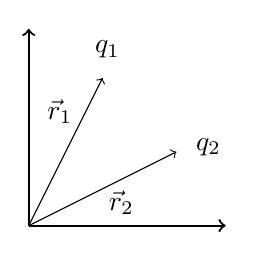
\begin{tikzpicture}
	\node at (1,2) (a) {};
	\node at (2,1) (b) {};
	\draw[thick,->] (0,0) -- (0,2.5);
	\draw[thick,->] (0,0) -- (2.5,0);
	\draw[->] (0,0) -- (a) node[above] {$ q_1 $};
	\draw[->] (0,0) -- (b) node[right] {$ q_2 $};
	\node at (.5,1) (c) {};
	\node at (1,.5) (d) {};
	\draw[] (c) node[above,yshift=5,xshift=-3] {$ \vec{r}_1 $};
	\draw[] (d) node[below,yshift=2,xshift=5] {$ \vec{r}_2 $};
	\end{tikzpicture}
\end{minipage}

\begin{enumerate}
	\item $\vec{F}_{12} \sim q_1 q_2$
	\item $\vec{F}_{12} \sim \frac{1}{|\vec{r}_1 - \vec{r}_2|^2}$
	\item $\vec{F}_{12} \sim q_1 q_2\, \vec{e}_{r_{12}}$
	\item $\vec{F}_{12} = -\vec{F}_{21}$
\end{enumerate}
Es gilt das Superpositionsprinzip: Das heißt, durch vektorielle Addition der Kräfte kann die Gesamtkraft ermittelt werden.

$$\vec{F}_1 = k \summ{j = 2}{N} \frac{q_1 q_j}{r_{1j}^2}\vec{e}_{r_{1j}}$$

\paragraph{Zur Konstanten $k$:}

Die Konstante ist abhängig von dem verwendeten Maßsystemen.
\begin{enumerate}[i)]
	\item Gauß-System (cgs): $k \equiv 1$, dyn = $\frac{\textrm{g}\cdot \textrm{cm}}{\textrm{s}^2} = 10^{-5}\,\textrm{N}$\\
	1 dyn = $\frac{(1\textrm{ESE})^2}{\textrm{cm}^2} \quad 1\textrm{ESE} = \frac{\sqrt{\textrm{g}\cdot \textrm{cm}^3}}{\textrm{s}}$
	\item SI (MKSA-System): Definition von A = Amp\`ere 
	%t4:
	\vspace{-15pt}
	$$\frac{\Delta F}{\Delta l}= 2 \cdot 10^{-7}\,\frac{\textrm{N}}{\textrm{m}} \qquad \qquad 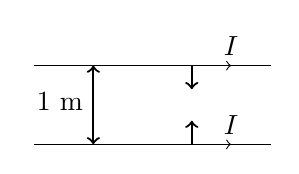
\begin{tikzpicture}
	\draw (0,0) -- (3,0);
	\draw (0,1) -- (3,1);
	\draw[thick,<->] (.75,0) -- (.75,1) node[anchor=north east,yshift=-6pt] {1 m};
	\draw[thick,->] (2,0) -- (2,.3);
	\draw[thick,->] (2,1) -- (2,.7);
	\draw[->] (2,0) -- (2.5,0) node[above] {$ I $};
	\draw[->] (2,1) -- (2.5,1) node[above] {$ I $};
	\end{tikzpicture}$$
	Strom = $\frac{\textrm{Ladung}}{\textrm{Zeit}}$ $\Rightarrow$  \ 
	$
	1 \tx{A} = \frac{1 \tx{C}}{1 \tx{s}} \quad \rightarrow \quad e = 1{,}602 \cdot 10^{-19} \, \tx{C} \qquad c \approx 3 \cdot 10^{8} \, \frac{\tx{m}}{\tx{s}}
	$\\[5pt]
	$
	\frac{\Delta F}{\Delta l} = k \frac{2 I^2}{c^2 d} \qquad \rightarrow k = 2 \cdot 10^{-7} \ \frac{\tx{N}}{\tx{m}} \frac{c^2 1 \tx{m}}{2 (1 \tx{A})^2} = 10^{-7} c^2 \, \frac{\tx{N}}{\tx{A}^2}
	$
	\begin{equation*}
	k = \frac{1}{4 \pi \epsilon_0}
	\end{equation*}
	Damit erhalten wir für die Dielektrizitätskonstante des Vakuums:
	\begin{equation*}
	\epsilon_0 = 8{,}85 \cdot 10^{-12} \frac{\tx{C}^2}{\tx{N} \tx{m}^2}
	\end{equation*}
\end{enumerate}

\section{Elektrisches Feld}
\subsection{Feld eines Systems von Punktladungen}

\begin{minipage}{.5\linewidth}
	$N$-Ladungen $q_1, \dots, q_N$ ruhen an den Orten $\vec{r}_1, \dots, \vec{r}_N$. Nun bringen wir eine Testladung $q$ am Ort $\vec{r}$ mit ein. 
\end{minipage}%
\begin{minipage}{.5\linewidth}
	%t5:
	\hspace{50pt}
	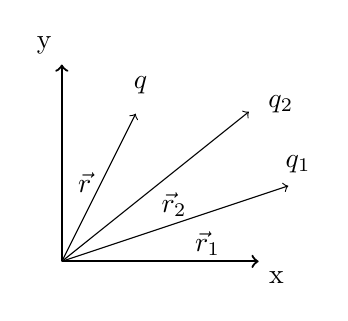
\begin{tikzpicture}
	\node at (3,1) (a) {};
	\node at (2.5,2) (b) {};
	\node at (1,2) (c) {};
	\draw[thick,->] (0,0) -- (0,2.5) node[anchor=south east] {y};
	\draw[thick,->] (0,0) -- (2.5,0) node[anchor=north west] {x};
	\draw[->] (0,0) -- (a) node[above] {$ q_1 $};
	\draw[->] (0,0) -- (b) node[right] {$ q_2 $};
	\draw[->] (0,0) -- (c) node[above] {$ q $};
	\node at (1.5,.5) (c) {};
	\node at (1.25,1) (d) {};
	\node at (.5,1) (e) {};
	\draw[] (c) node[below,xshift=10pt] {$ \vec{r}_1 $};
	\draw[] (d) node[below,xshift=5pt] {$ \vec{r}_2 $};
	\draw[] (e) node[left] {$ \vec{r} $};
	\end{tikzpicture}
\end{minipage}%
\\
Kraft von $q_1,\ q_2$ auf $q$
$$\vec{F} = \frac{1}{4\pi \epsilon_0} q \summ{j = 1}{N} q_j \frac{\vec{r} - \vec{r}_j}{|\vec{r} - \vec{r}_j|^3} = q \vec{E}(\vec{r})$$
Somit ist das elektrisches Feld:
$$\rmbox{\vec{E}(\vec{r}) = \frac{1}{4 \pi \epsilon_0} \summ{j = 1}{N} q_j \frac{\vec{r} - \vec{r}_j}{|\vec{r} - \vec{r}_j|^3}}$$
\textbf{\emph{Bemerkung}}
\begin{enumerate}[i)]
	\item Testladung klein (formal: $ \lim_{q\to0}\frac{\vec{F}}{q} $)
	\item math. $ \vec{E}(\vec{r}) $ Vektorpfeil\\
	\begin{equation*}
	\tx{kartesisch:} \quad \vec{E}(\vec{r}) = \begin{pmatrix}
	E_x(\vec{r}) \\ E_y(\vec{r}) \\ E_z(\vec{r})
	\end{pmatrix}
	\end{equation*}
	\item Wechselwirkungsprozess: 2 Teile
	\begin{equation*}
	q_j \rightarrow \vec{E}(\vec{r}) \rightarrow \vec{F} = q \vec{E} (\vec{r})
	\end{equation*}
	\item Superpositionsprinzip gilt
\end{enumerate}

\subsection[Feld einer kontinuierlichen Ladungsverteilung]{Feld einer kontinuierlichen Ladungsverteilung $\rho(\vec{r})$}

\begin{minipage}{.7\linewidth}
	$$\rmbox{\vec{E}(\vec{r}) =\frac{1}{4 \pi \epsilon_0} \int\limits_V \dd^3 r'\, \rho(\vec{r}')\frac{\vec{r} - \vec{r}'}{|\vec{r} - \vec{r}'|^3}}$$
	$ \ub{\int\limits_V \dd ^3 r'}_{\mathclap{\substack{\tx{schließt alle} \\ \tx{Ladungen ein}}}} \qquad \rho(\vec{r}_j) = \frac{\Delta q_j}{\Delta V_j}$
\end{minipage}%
\begin{minipage}{.3\linewidth}
	\flushright
	%t6:
	\begin{tikzpicture}
	\node at (1.5,1.5) (a) {};
	\draw  plot [smooth cycle, tension=1] coordinates { (0,0) (.5,1) (.5,2.5) (2,2.2) (3,2) (2.5,.5) (1.5,-.2) };
	\pic at (a) {annotated cuboid={width=3,height=3,depth=3}};
	\draw[] (a) node[right,xshift=10pt] {$ \Delta V_j $};
	\draw[] (a) node[right,xshift=-10pt,yshift=10pt] {$ \Delta q_j $};
	\draw[->] (3,.5) to[out=180,in=-40] (2.2,.8);
	\node[right] at (3,.5) (b) {$ V $};
	\draw[thick,->] (-.5,-.5) -- (-.5,2) node[anchor=south east] {y};
	\draw[thick,->] (-.5,-.5) -- (2,-.5) node[anchor=north west] {x};
	\draw[thick,->] (-.5,-.5) -- (.25,.25) node[anchor=south east] {z};
	\draw[] (1,0) node[above] {$ \rho(\vec{r}) $};
	\end{tikzpicture}
\end{minipage}%

\begin{align*}
\vec{E}(\vec{r}) &= k\sum_j\Delta q_j\frac{\vec{r}-\vec{r}_j}{|\vec{r}-\vec{r}_j|^3}\\
&= k\sum_j\Delta V_j\rho(\vec{r}_j)\frac{\vec{r}-\vec{r}_j}{|\vec{r}-\vec  {r}_j|^3}\\
\scriptstyle{\tx{mit } \Delta V_j \to 0}\ \ &= k\int_V \dd^3r'\rho(\vec{r}')\frac{\vec{r}-\vec{r}'}{|\vec{r}  -\vec{r}'|^3}
\end{align*}

% Vorlesung 2 %18.10.18

\subsection{Ladungsdichte einer Punktladung}

\begin{minipage}{.6\linewidth}
	\paragraph{Deltafunktion}
	
	$$\rho (\vec{r}) = q \delta(\vec{r}-\vec{r}_0)$$
	Punktladung in $\vec{r}_0 \Rightarrow \rho(\vec{r}) = 0 \quad \vec{r} \neq \vec{r}_0$\\
	Ladungsdichte divergiert in $\vec{r}_0$
	$$\rho(\vec{r}_0) = \infty$$
\end{minipage}%
\begin{minipage}{.4\linewidth}
	%t1:
	\centering
	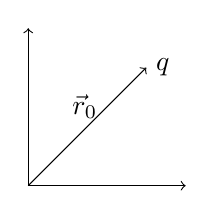
\begin{tikzpicture}
	\draw[->] (0,0) -- (0,2);
	\draw[->] (0,0) -- (2,0);
	\draw[->] (0,0) -- (1.5,1.5) node [right] {$q$};
	\draw (1,1) node [above,left] {$\vec{r}_0$};
	\end{tikzpicture}
\end{minipage}%
\\
Modell für Punktladung:\\
Ladung $q$ in Kugel mit Radius $\epsilon$  um $\vec{r}_0,\ \epsilon \rightarrow 0$
$$\rho_2 (\vec{r}) = \left\{ \begin{array}{cc}
\frac{q}{v_k} & |\vec{r}| \leq \epsilon\\
0 & \textrm{sonst}	
\end{array} \right\} = \frac{q}{\frac{4}{3}\pi \epsilon^3}\underbrace{\Theta (\epsilon - |\vec{r}|)}_{\mathclap{\textrm{Stufenfunktion}}}$$
%
%
%
% I1 T?
%
%
%
$$\rho(\vec{r}) = \lim_{\epsilon \rightarrow 0}\ \rho_\epsilon (\vec{r}) = \left\{ \begin{array}{cc}
\infty & \vec{r} = 0\\
0 & \vec{r} \neq 0
\end{array}\right.$$
Divergenz muss so sein, dass $$ \int\limits_{\substack{V \\ \vec{r}_0 \in V}} \dd^3r\ \rho(\vec{r}) = q$$

\paragraph{Definition Delta-Funktion (Diracsche Deltafunktion)}

\begin{enumerate}
	\item 
	$$\delta (\vec{r} - \vec{r}_0) = \left\{ \begin{array}{cc}
		0 & \vec{r} \neq \vec{r}_0 \\
		\infty & \vec{r} = \vec{r}_0
	\end{array}\right.$$
	\item 
	$$\int_V \dd^3 r\ f(\vec{r}) \delta(\vec{r} - \vec{r}_0) = \left\{ \begin{array}{cc}
		f(\vec{r}_0) & \vec{r}_0 \in V\\
		0 & \vec{r}_0 \notin V
	\end{array}\right.$$ 
\end{enumerate}

\paragraph{Mathematik}
Distribution - Funktional\\[5pt]
Funktional: Abb. Funktionen $\mapsto \mathbb R, \mathbb C$
$$\delta_{\vec{r}_0}: f \mapsto f(\vec{r}_0)$$

\paragraph{Physik}

$$\int \dd^3 r\ f(\vec{r}) \delta (\vec{r}-\vec{r}_0) = f(\vec{r})$$
$\delta$-Fkt. als Grenzwert einer Folge von Funktionen im Integral
$$\int \dd^3 r\ f(\vec{r}) \delta (\vec{r} - \vec{r}_0) = \lim_{\epsilon \to 0} \quad \int \dd^3 r\ f(\vec{r}) g_\epsilon(\vec{r}-\vec{r}_0) $$
mit
$$\lim_{\epsilon \to 0} g_\epsilon (\vec{r}-\vec{r}_0) =  \left\{ \begin{array}{cc}
0 & \vec{r} \neq \vec{r}_0 \\
\infty & \vec{r} = \vec{r}_0
\end{array}\right.$$
$$\int_V \dd^3 r\ g_\epsilon (\vec{r}-\vec{r}_0) = 1$$
\emph{Beispiel:} $g_\epsilon (\vec{r}-\vec{r}_0) = \frac{\Theta(\epsilon - |\vec{r}|)}{\frac{4}{3}\pi \epsilon^3}$\\
Mehrere Punktladungen $q_j$ in $\vec{r}_j$
$$\rho(\vec{r}) = \sum_j q_j \delta(\vec{r}-\vec{r}_j)$$

\begin{align*}
 	\Rightarrow \vec{E}(\vec{r}) &= \kq \int_V \dd^3 r'\ \rho(\vec{r}') \frac{\vec{r} - \vec{r}'}{|\vec{r} - \vec{r}'|^3}\\
	&= \kq \int_V \dd^3 r'\ \sum_j q_j \delta(\vec{r} - \vec{r}_j) \frac{\vec{r} - \vec{r}'}{|\vec{r} - \vec{r}'|^3}\\
	&= \kq \sum_j q_j \int_V \dd^3 r'\ \delta(\vec{r} - \vec{r}_j) \frac{\vec{r} - \vec{r}'}{|\vec{r} - \vec{r}'|^3}\\
	&= \kq \sum_j q_j \frac{\vec{r} - \vec{r}_j}{|\vec{r} - \vec{r}_j|^3} \qquad \checkmark\\
\end{align*}

\subsection{Flächenladungsdichte}

\begin{minipage}{.5\linewidth}
	$\sigma(\vec{r}) = \frac{\textrm{Ladung}}{\textrm{Fläche}} = \frac{\Delta q}{\Delta A}$
\end{minipage}%
\begin{minipage}{.5\linewidth}
	%t2 eig %t1:
	\centering
	\begin{tikzpicture}
		\draw[->] (0,0) -- (0,1);
		\draw[->] (0,0) -- (1,0);
		\draw[->] (0,0) -- (-.5,-.5);
		\draw (.5,.2) -- ++(30:1.3) -- ++(90:1) -- ++(-150:1.3) -- (.5,.2);
		\draw (.9,.7) -- ++(30:.3) -- ++(90:.3) -- ++ (-150:.3) -- (.9,.7);
		\draw[thick,->] (0,0) -- (.9,.7) node[yshift=-7pt,xshift=-18pt] {$ \vec{r} $};
		\draw ($ (.9,.7) + (30:.3) + (90:.3) + (-120:.15) $) to[out=65,in=150] (2,2) node[right] {$ \Delta A $};
		\draw ($ (.5,.2) + (33:1.1) $) to[out=-50,in=-150] (2,.5) node[right] {$ A $};
		\draw ($ (.9,.7) + (30:.3) + (90:.3) + (-100:.2) $) to[out=20,in=180] (2.2,1.35) node[right] {$ \Delta q $};
	\end{tikzpicture}
\end{minipage}%
\\
erzeugtes elektrisches Feld:
$$\vec{E}(\vec{r}) = \kq \int\limits_A \underbrace{\dd f'}_{\mathclap{\substack{\textrm{Flächen-} \\ \tx{element}}}}\ \sigma (\vec{r}) \frac{\vec{r} - \vec{r}'}{|\vec{r} - \vec{r}'|^3}$$
\begin{minipage}{.65\linewidth}
	\bei Elektrisches Feld einer homogenen Flächenladung
\end{minipage}%
\begin{minipage}{.35\linewidth}
	%t3 eig %t2:
	\centering
	\begin{tikzpicture}
		\draw[->] (0,0) -- (0,1) node[anchor=south east] {$ z $};
		\draw[->] (0,0) -- (2,0) node[anchor=north west] {$ y $};
		\draw[->] (0,0) -- (-1,-1) node[anchor=north east] {$ x $};
		\node at (2,1) {$ \substack{\sigma = \const \tx{in} \\ x\tx{-}y \tx{-Ebene} } $};
		\draw (-.3,-.3) -- ++(1.8,0);
		\draw (-.6,-.6) -- ++(1.8,0);
		\draw (-.9,-.9) -- ++(1.8,0);
		\draw (1.8,0) -- ++(-.9,-.9);
		\draw (1.2,0) -- ++(-.9,-.9);
		\draw (.6,0) -- ++(-.9,-.9);
	\end{tikzpicture}
\end{minipage}%
$$\vec{E}(\vec{r}) = \kq \intt{-\infty}{+\infty}\dd x'\intt{-\infty}{+\infty}\dd y'\ \sigma \frac{\vec{r} - \vec{r}'}{|\vec{r} - \vec{r}'|^3} \qquad \vec{r}' = (x', y', 0)$$
Symmetrie: $\vec{E}$ unabhängig von $x,y \qquad \vec{r} = (0,0,z)$
$$\vec{r} - \vec{r}' = (-x',-y',z),\ |\vec{r} - \vec{r}'|^3 = (x'^2+y'^2+z^2)^{\nicefrac{3}{2}}$$
$$E_x \sim \sigma \intt{-\infty}{+\infty}\dd x'\intt{-\infty}{+\infty}\dd y'\ \frac{(-x')}{(x'^2 + y'^2 + z^2)^{\nicefrac{3}{2}}} = 0 = E_y$$

$\vec{E} = (0,0,E_z)$

\begin{align*}
 	E_z &= \kq \sigma_z \intt{-\infty}{+\infty}\dd x'\underbrace{\intt{-\infty}{+\infty}\dd y'\ \frac{(x')}{(x'^2 + y'^2 + z'^2)^{\nicefrac{3}{2}}}}\\
 	& \qquad \frac{1}{x'^2 +z^2}\left.\frac{y'}{(x'^2 + y'^2 + z^2)^{\nicefrac{3}{2}}} \right\rvert_{-\infty}^{+\infty} = \frac{1}{x'^2 +z^2}\left.\frac{\textrm{sgn}(y')}{\sqrt{1 + \frac{x'^2 + z^2}{y'^2}}} \right\rvert_{-\infty}^{+\infty} = \frac{2}{x'^2 +z^2}\\
 	&= \frac{1}{2 \pi \epsilon_0} \sigma_z \underbrace{\intt{-\infty}{+\infty} \dd x'\ \frac{1}{x'^2 + z^2}}_{\left. \frac{1}{z} \arctan \left(\frac{x'}{2}\right)\right\rvert_{-\infty}^{+\infty} = \frac{1}{z} \textrm{sgn}(z)\pi}\\
 	E_z &= \frac{\sigma}{2 \epsilon_0} \textrm{sgn}(z)
\end{align*}
\begin{minipage}{.6\linewidth}
	Grenzfläche: $z \rightarrow 0$
	$$\vec{E} \underset{z \to 0} \longrightarrow \left\{ \begin{array}{cc}
	\frac{\sigma}{2 \epsilon_0} \vec{e}_z & z > 0\\
	-\frac{\sigma}{2 \epsilon_0} \vec{e}_z & z < 0
	\end{array}\right.$$
	$$\vec{E}_{\perp_+} - \vec{E}_{\perp_-} = \frac{\sigma}{\epsilon_0}, \qquad \vec{E}_\parallel = 0$$
\end{minipage}%
\begin{minipage}{.4\linewidth}
	%t3:
	\centering
	\begin{tikzpicture}
		\draw[->] (0,-1.2) -- (0,1.2) node[above] {$ E_z $};
		\draw[->] (-2,0) -- (2,0) node[anchor=north west] {$ z $};
		\draw[thick] (2,.8) -- (0,.8) ;
		\draw (0,.8) -- (-.15,.8) node[left] {$ \frac{\sigma}{2 \epsilon_0} $};
		\draw[thick] (-2,-.8) -- (0,-.8);
		\draw (0,-.8) -- (.15,-.8) node[right] {$\frac{\sigma}{2 \epsilon_0}$};
	\end{tikzpicture}
\end{minipage}%
%t4: %t5:
\begin{center}
\begin{tikzpicture}
	\coordinate (o) at (-8,0);
	\draw[thick,->] ($ (o) + (-.5,0)$) -- ++(2.5,0) node[anchor=north west] {$ z $};
	\draw[very thick] ($ (o) + (0,-1) $) -- ++(0,2) node[above] {$ \sigma $};
	\draw[very thick] ($ (o) + (1.5,-1) $) -- ++(0,2) node[above] {$ -\sigma $};
	
	\draw[->] (-2,0) -- (2,0) node[anchor=north west] {$ z $};
	\draw[->] (0,-1) -- (0,1.5) node[anchor=south east] {$ E_z $};
	\draw[very thick] (-2,0) -- (-.75,0);
	\draw[very thick] (.75,0) -- (2,0);
	\draw[very thick] (-.75,1) -- (.75,1) node[anchor=south west] {$ \frac{\sigma}{\epsilon_0} $};
	\draw[ultra thick,draw=orange,dashed] (-2,.5) -- (.75,.5);
	\draw[ultra thick,draw=orange,dashed] (.75,-.5) -- (2,-.5) node[right] {$ - \sigma $};
	\draw[very thick,draw=black!25!green,dashed] (-.75,-.5) -- (-2,-.5) node[left] {$ \sigma $};
	\draw[very thick,draw=black!25!green,dashed] (2,.5) -- (-.75,.5);
	\draw (.75,-.1) -- (.75,.1);
	\draw (-.75,-.1) -- (-.75,.1);
	\draw (-.1,.5) -- (.1,.5) node[right,xshift=55pt] {$ \frac{\sigma}{2 \epsilon_0} $};
	\draw (-.1,-.5) -- (.1,-.5) node[right,xshift=-2pt] {$ \frac{- \sigma}{2 \epsilon_0} $};
\end{tikzpicture}
\end{center}

\subsection{Linenladungsdichte}

\begin{minipage}{.5\linewidth}
	$$\lambda(\vec{r}) = \frac{\textrm{Ladung}}{\textrm{Länge}} = \frac{\Delta q}{\Delta s}$$
	$$\vec{E}(\vec{r}) = \kq \underbrace{\int\limits_\gamma}_{\mathclap{\textrm{Linienintegral}}} \dd s'\ \lambda(\vec{r}') \frac{\vec{r} - \vec{r}'}{|\vec{r} - \vec{r}'|^3}$$
\end{minipage}%
\begin{minipage}{.5\linewidth}
	%t6:
	\centering
	\begin{tikzpicture}
		\draw[->] (0,0) -- (0,1);
		\draw[->] (0,0) -- (1,0);
		\coordinate (m) at (2,3);
		\draw[thick,->] (0,0) -- (m) node[xshift=-30pt,yshift=-35pt] {$ \vec{r} $};
		\draw ($ (m) + (45:0.2) $) -- ++(180:.3) node[anchor=south east] {$ \Delta s $} -- ++(-90:.3) -- ++(0:.3) -- ++(90:.3) node[anchor=north west] {$ \Delta q $};
		\draw[thick] (-.5,1.5) to[out=80,in=-170] (1,2.7) to[out=10,in=-160] (m) to[out=20,in=-100] (3,4) node[right] {$ \gamma $};
	\end{tikzpicture}
	\vspace{15pt}
\end{minipage}%
\\
\emph{Beispiel:} Elektrisches Feld einer homogenen Linienladung $ \lambda = \const $\\
\begin{minipage}{.2\linewidth}
	%t7:
	\centering
	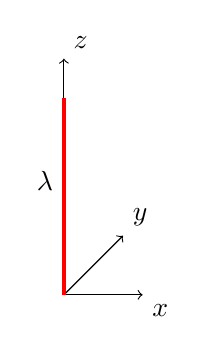
\begin{tikzpicture}
		\draw[->] (0,0) -- (1,0) node[anchor=north west] {$ x $};
		\draw[->] (0,0) -- (.75,.75) node[anchor=south west] {$ y $};
		\draw[->] (0,0) -- (0,3) node[anchor=south west] {$ z $};
		\draw[very thick,draw=red] (0,0) -- (0,2.5) node[left,yshift=-30pt] {$ \lambda $};
	\end{tikzpicture}
\end{minipage}%
\begin{minipage}{.8\linewidth}
	\begin{align*}
	\vec{E}(\vec{r}) &= \kq \int_\gamma \dd s'\ \lambda \frac{\vec{r} - \vec{r}'}{|\vec{r} - \vec{r}'|^3} \qquad \gamma: z' \mapsto \vec{r}'(z') = \begin{pmatrix} 0 \\ 0 \\ z' \end{pmatrix}\\
	% I2:
	&= \frac{\lambda}{4 \pi \epsilon_0} \intt{-\infty}{\infty}\dd z'\ \frac{\vec{r} - \begin{pmatrix} 0 , 0 , z \end{pmatrix}^\top}{(x^2 + y^2 + (z-z')^2)^{\nicefrac{3}{2}}}
	\end{align*}
\end{minipage}%
\\
$\tilde{z} = z' - z$:
$$E_x = \frac{\lambda x}{4 \pi \epsilon_0}\intt{-\infty}{\infty} \dd z'\ \frac{1}{(x^2 + y^2 + (z-z')^2)^{\nicefrac{3}{2}}} = \frac{\lambda x}{4 \pi \epsilon_0}\underbrace{\intt{-\infty}{\infty}\dd\tilde{z}\ \frac{1}{(x^2 + y^2 + \tilde{z}^2)^{\nicefrac{3}{2}}}}_{\frac{2}{x^2 + y^2}} = \frac{\lambda}{2 \pi \epsilon_0} \frac{x}{x^2 + y^2}$$
Wegen der Symmetrie genau so:
$$E_y = \frac{\lambda}{2 \pi \epsilon_0}\frac{x}{x^2 + y^2}$$
$$E_z = \frac{\lambda}{4 \pi \epsilon_0} \intt{-\infty}{\infty}\dd z'\ \frac{z-z'}{(x^2 + y^2 + (z-z')^2)^{\nicefrac{3}{2}}} = 0$$
$$\vec{E}(\vec{r}) = \frac{\lambda}{2 \pi \epsilon_0} \frac{1}{x^2 + y^2} \begin{pmatrix}x\\ y\\ 0\end{pmatrix}$$
$$\rho = \sqrt{x^2 + y^2} \quad \vec{E}(\vec{r}) = \frac{\lambda}{2 \pi \epsilon_0} \frac{1}{\rho}\vec{e}_\rho, \qquad \vec{e}_\rho = \begin{pmatrix}\cos \varphi\\ \sin \varphi\\ 0\end{pmatrix}$$

\section{Feldgleichungen und elektrostatisches Potential}

$$\vec{E}(\vec{r}) = \kq \int \dd^3 r'\ \rho(\vec{r}') \frac{\vec{r} - \vec{r}'}{|\vec{r} - \vec{r}'|^3}$$

\subsection{Elektrostatisches Potential}

elektrische Feld ist ein Potentialfeld $\vec{E}(\vec{r}) = - \vabla\phi(\vec{r}) = - \bigg( \vec{e}_x \prt{\phi}{x} + \vec{e}_y \prt{\phi}{y} + \vec{e}_z \prt{\phi}{z}\bigg)$\\
Nebenrechnung:
$$\frac{\vec{r} - \vec{r}'}{|\vec{r} - \vec{r}'|^3} = -\vabla\frac{1}{|\vec{r}-\vec{r}'|}$$
zur Überprüfung hier die $ x $-Komponente berechnet:
$$-\prt{}{x} \frac{1}{[(x-x')^2 + (y-y')^2 + (z-z')^2]^{\nicefrac{1}{2}}} =  \frac{- \left(-\frac{1}{2}\right) \quad 2(x-x')}{[(x-x')^2 + (y-y')^2 + (z-z')^2]^{\nicefrac{3}{2}}} = \frac{(x-x')}{|\vec{r} - \vec{r}'|^3}$$
Somit erhalten wir für das $ \vec{E} $-Feld:
$$\Rightarrow \vec{E}(\vec{r}) = \kq \int \dd^3 r'\ \rho(\vec{r}') \bigg(-\vabla_{\vec{r}} \frac{1}{|\vec{r} - \vec{r}'|} \bigg) = (-) \vabla_{\vec{r}} \kq \int \dd^3 r'\ \frac{\rho(\vec{r}')}{|\vec{r} - \vec{r}'|}$$
% I3:
$\rightarrow$ elektrostatisches Potential
$$\phi(\vec{r}) = \kq \int \dd^3 r'\ \frac{\rho(\vec{r}')}{|\vec{r} - \vec{r}'|} + c$$
übliche Konvention: $c = 0 \quad (\phi(\vec{r})\buildrel{|\vec{r}| \to \infty}\over{\rightarrow} 0)$\\[5pt]
\emph{Beispiel:} Potential einer Punktladung in $\vec{r}_0$:
$$\rho(\vec{r}) = q \delta(\vec{r}-\vec{r}_0)$$
$$\phi(\vec{r}) = \frac{1}{4 \pi \epsilon_0} \int_{\mathbb R^3} \dd^3 r'\ \frac{q\delta(\vec{r}' - \vec{r}_0)}{|\vec{r}-\vec{r}'|} = \kq \frac{q}{|\vec{r} - \vec{r}_0|}$$
$$\eofr = - \vabla \phi = \kq q \vabla \frac{1}{|\vec{r} - \vec{r}_0|} = \kq q \frac{\vec{r} - \vec{r}_0}{|\vec{r} - \vec{r}_0|^3}$$

% Vorlesung 3 22.10.18

\noindent
\lcom{(Funktional-Analysis Siegfried Großmann Springer)\\
(Landau-Lipschitz Buch geht weit der Vorlesung hinaus)}
%
%
%
% I4 T äquipotentialflächen jan
%
%
%
\subsection{Feldgleichung (differentielle Form)}

\paragraph{Rotation (Wirbel)}
$$\textrm{rot}\, \vec{E} =  \vabla \times \vec{E} = \vec{e}_x \bigg(\prt{E_z}{y} - \prt{E_y}{z}\bigg) + \vec{e}_y \bigg(\prt{E_x}{z} - \prt{E_z}{x}\bigg) + \vec{e}_z \bigg(\prt{E_y}{x} - \prt{E_x}{y}\bigg)$$
$$\Rightarrow \vabla \times \vec{E} = - \vabla \times (\vabla\phi) = 0$$
Mathe: Sie sind äquivalent
\begin{enumerate}[i)]
	\item $\vec{E} = - \vabla\phi$
	\item $\vabla \times \vec{E} = 0$ (auf einfach zusammenhängendem Gebiet)
	\item Kurvenintegral $\int_\gamma \dd\vec{r} \cdot \vec{E}$ ist Wegunabhängig 
	%
	%
	%
	% I5 T1
	%
	%
	%
	$$\intt{\vec{r}_1}{\vec{r}_2} \dd\vec{r} \cdot \vec{E} = - \intt{\vec{r}_1}{\vec{r}_2} \dd t \underbrace{\frac{\dd\vec{r}}{\dd t}\times \vabla\phi(\vec{r}(t))}_{\frac{\dd\phi}{\dd t}} = \underbrace{(\phi(\vec{r}_2) - \phi(\vec{r}_1))}_{\textrm{Potentialdifferenz}} $$
\end{enumerate}

\paragraph{Divergenz (Quellen)}

$$\tx{div} \vec{E} = \vabla \cdot \vec{E} = \prt{E_x}{x} + \prt{E_y}{y} + \prt{E_z}{z}$$
\begin{align*}
\vabla \cdot \vec{E}(\vec{r}) &= \vabla_{\vec{r}} \cdot \kq \int\dd^3r'\ \rho(\vec{r}') \frac{1}{|\vec{r} - \vec{r}'|^3}\\
&= \kq \int_V \dd^3 r' \rho (\vec{r}') \vabla_{\vec{r}} \cdot \frac{1}{|\vec{r} - \vec{r}'|^3}
\end{align*}
$x$-Anteil:
\begin{align*}
\frac{\partial}{\partial x}\frac{x-x'}{[(x-x')^2 + (y-y')^2 + (z-z')^2]^{\nicefrac{3}{2}}} &= \frac{1 \cdot [\dots]^{\nicefrac{3}{2}}(x - x')(x - x')^{\nicefrac{3}{2}}\cdot 2[\dots]^{\nicefrac{1}{2}}}{[\dots]^3}\\
&= \frac{[\dots]^{\nicefrac{1}{2}}((x - x')^2 + (y - y')^2 + (z - z')^2 - 3(x - x')^2)}{[\dots]^{\nicefrac{3}{2}}}\\
&= \frac{(y - y')^2 + (z - z')^2 - 2(x - x')^2}{[\dots]^{\nicefrac{3}{2}}}
\end{align*}
$$\frac{\partial}{\partial y} \frac{y-y'}{[(x-x')^2 + (y-y')^2 + (z-z')^2]^{\nicefrac{3}{2}}} = \frac{(x - x')^2 + (z - z')^2 - 2(y - y')^2}{[\dots]^{\nicefrac{3}{2}}}$$ 
$$\frac{\partial}{\partial z} \frac{z-z'}{[(x-x')^2 + (y-y')^2 + (z-z')^2]^{\nicefrac{3}{2}}} = \frac{(x - x')^2 + (y - y')^2 - 2(z - z')^2}{[\dots]^{\nicefrac{3}{2}}}$$ 
$$\vabla \cdot \frac{\vec{r} - \vec{r}'}{|\vec{r} - \vec{r}'|^3} = 0 \quad \textrm{falls} \quad \vec{r} \neq \vec{r}'$$
$$\Rightarrow \textrm{falls} \quad \vec{r} \notin V, \textrm{ d.h. } \vec{r} \textrm{ in Gebiet ohne Ladungsdichte } \rho(\vec{r}) = 0$$
$$\Rightarrow \vabla \cdot \vec{E}(\vec{r}) = 0$$ 
%
%
%
% I6 T?
%
%
%
$\vec{r} \in V$: Grenzwertbetrachtung (Regularisierung des Integranden)\\
statt
$$\frac{\vec{r} - \vec{r}'}{|\vec{r} - \vec{r}'|^3} = \frac{\vec{r}-\vec{r}'}{[(x-x')^2 + (y-y')^2 + (z-z')^2]^{\nicefrac{3}{2}}}$$
betrachten wir:
$$f_a (\vec{r}-\vec{r}') = \frac{\vec{r}-\vec{r}'}{[(x-x')^2 + (y-y')^2 + (z-z')^2]^{\nicefrac{3}{2}}} = \frac{\vec{r}-\vec{r}'}{[(\vec{r}-\vec{r}')^2 + a^2]^{\nicefrac{3}{2}}} \quad a \in \mathbb R,\ a>0$$
am Ende Grenzwert $\displaystyle{\lim_{a \to 0}}$
$$\vabla \cdot \vec{E} (\vec{r}) = \kq \lim_{a \to 0} \int_V \dd^3r'\ \rho(\vec{r}')\ \rmbox{\hspace{-10pt}\vabla_{\vec{r}}\cdot f_a(\vec{r}-\vec{r}')}$$

\begin{align*}
\prt{}{x} \frac{x-x'}{[(\vec{r}-\vec{r}')^2 + a^2]^{\nicefrac{3}{2}}} &= \frac{[\dots +a^2]^{\nicefrac{3}{2}} - (x - x') \frac{3}{2} \cdot 2(x-x') [\dots + a^2]^{\nicefrac{3}{2}}}{[\dots + a^2]^3}\\
&= \frac{(y - y')^2 + (z - z')^2 + a^2 - 2(x - x')^2}{[\dots + a^2]^{\nicefrac{3}{2}}}
\end{align*}

$$\vabla_{\vec{r}} \cdot f_a(\vec{r}-\vec{r}') = \frac{3a^2}{[(\vec{r}-\vec{r}')^2 + a^2]^{\nicefrac{5}{2}}}$$
$$\lim_{a \to 0} f_a(\vec{r}-\vec{r}') = \left\{ \begin{array}{cc}
0 & \vec{r} \neq \vec{r}'\\
\infty & \vec{r} = \vec{r}'	
\end{array} \right.$$
%
%
%
% I7  muss beim limes ein vabla_r \cdot hin ?
%
%
%
$$\Rightarrow \textrm{zum Integral } \int_V \dd^3r' \dots \textrm{ trägt (im Limes }a \to 0) \textrm{ nur der Bereich } \vec{r}' \approx \vec{r} \textrm{ bei}$$
$$K_R (\vec{r}) = \{\vec{r}' \in \mathbb R^3: |\vec{r} - \vec{r}'| \leq R\}$$
%
%
%
% I8 T zum integral jan
%
%
%
\begin{align*}
 	\hspace{100pt} &\lim_{a \to 0} \int_V \dd^3 r'\ \rho(\vec{r}') \vabla_{\vec{r}} \cdot f_a(\vec{r}- \vec{r}')\\
	&= \lim_{a \to 0} \int_{K_R (\vec{r})} \dd^3 r' \ \rho(\vec{r}') \frac{3a^2}{[(\vec{r}-\vec{r}')^2 + a^2]^{\nicefrac{5}{2}}}\\
 	&+ \underbrace{\lim_{a \to 0} \int_{V / K_R (\vec{r})} \dd^3 r' \rho(\vec{r}') \frac{3a^2}{[(\vec{r}-\vec{r}')^2 + a^2]^{\nicefrac{5}{2}}}}_{= 0}
\end{align*}
Wähle $R$ klein genug, dass man innerhalb $K_R (\vec{r})$, $\rho(\vec{r}')$ in Taylorreihe um $\vec{r}$ entwickeln kann.
$$\vec{\tilde{r}} = \vec{r}' - \vec{r},\ \dd^3 r' = \dd^3 \tilde{r}$$
$$\int_{K_R (\vec{r})} \dd^3 r' \ \rho(\vec{r}') \frac{3a^2}{[(\vec{r}-\vec{r}')^2 + a^2]^{\nicefrac{5}{2}}} = \int_{K_R (0)} \dd^3 \tilde{r} \ \rho(\vec{r} + \vec{\tilde{r}}) \frac{3a^2}{[\vec{\tilde{r}}^2 + a^2]^{\nicefrac{5}{2}}}$$
Taylorentwicklung von $\rho(\vec{r} + \vec{\tilde{r}})$ um $\vec{\tilde{r}} = 0$
$$\rho(\vec{r} + \vec{\tilde{r}}) = \rho(\vec{r}) + \vec{\tilde{r}} \cdot \vabla \rho(\vec{r}) + \dots$$
$$\hspace{8.1cm} = \int_{K_R (0)} \dd^3 \tilde{r} \ (\rho(\vec{r}) + \vec{\tilde{r}} \cdot \vabla \rho(\vec{r}) + \dots) \frac{3a^2}{[\vec{\tilde{r}}^2 + a^2]^{\nicefrac{5}{2}}}$$
\begin{enumerate}
	\item Integral:
	\begin{align*}
	\int_{K_R (0)} \dd^3 \tilde r\ \rho(\vec{r}) \frac{3a^2}{(\tilde{r}^2 + a^2)^{\nicefrac{5}{2}}} &= \rho(\vec{r}) \underbrace{\intt{0}{R} \dd\tilde r\ \frac{3a^2}{(\tilde{r}^2 + a^2)^{\nicefrac{5}{2}}}}_{\left[\frac{\tilde r^3}{(\vec{\tilde{r}}^2 + a^2)^{\nicefrac{3}{2}}}\right]_0^R} \underbrace{\int \dd \equaltoup{\Omega}{\mathclap{\sin \theta \dd \theta \dd \varphi}}}_{= 4\pi}\\
	&= 4 \pi \rho(\vec{r}) \frac{R^3}{(R^2 + a^2)^{\nicefrac{3}{2}}} \quad \underset{a \to 0}{\longrightarrow} \quad 4 \pi \rho(\vec{r})
	\end{align*} 
	\item Integral:
	$$\int_{K_R (0)} \dd^3 \tilde{r}\ \equalto{\vec{\tilde{r}}}{\tilde{r}\vec{e}_{\vec{\tilde{r}}}} \cdot \vabla_{\vec{r}} \rho(\vec{r}) \frac{3 a^2}{(\tilde{r}^2 + a^2)^{\nicefrac{5}{2}}} = \underbrace{\intt{0}{R} \dd \tilde r\ \frac{3a^2 \tilde r^3}{(\tilde r^2 + a^2)^{\nicefrac{3}{2}}}}_{\frac{2}{3}a -3a^2 \left(\frac{R^2 +\frac{2}{3}a^2}{(R^2 + a^2)^{\nicefrac{3}{2}}}\right)} \underbrace{\int \dd \Omega\ \vec{e}_{\tilde{r}} \cdot \vabla \rho(\vec{r})}_{\textrm{unabh. von } a} \quad \underset{a \to 0}{\longrightarrow} \quad 0$$
	Das gilt auch für alle höheren Terme. Alle höheren Terme werden im Limit $ \lim_{a \to 0} $$ = 0 $.
	%
	%
	%
	% I9 wo kommt oben das \tilde{r} ^3 her ?
	%
	%
	%
\end{enumerate}

$$\lim_{a \to 0} \int_V \dd^3 r' \rho(\vec{r}) \vabla_{\vec{r}}\cdot \frac{(\vec{r}-\vec{r}')}{[(\vec{r}-\vec{r}')^2 + a^2]^{\nicefrac{3}{2}}} = 4 \pi \rho (\vec{r})$$
$$\Rightarrow \vabla \cdot \vec{E}(\vec{r}) = \kq \lim_{a \to 0} = \frac{1}{\epsilon_0} \rho(\vec{r})$$
\begin{center}
	\begin{minipage}{.5\linewidth}
		\rbox{$$\vabla \cdot \vec{E}(\vec{r}) = \frac{1}{\epsilon_0} \rho(\vec{r}) \quad \vec{r} \in \mathbb R^3$$}
	\end{minipage}
\end{center}

\subsection{Zusammenfassung:}

\paragraph{Feldgleichungen der Elektrostatik}
Mathe: partielle DGL
\rbox{
$$\vabla \cdot \vec{E}(\vec{r}) = \frac{1}{\epsilon_0} \rho(\vec{r}) \textrm{ inhomogene DGL}$$
$$\vabla \times \vec{E}(\vec{r}) = 0\textrm{ homogene DGL}$$}
\noindent
DGL für Potential $\phi$: 
$\vec{E} = - \vabla \phi$
\begin{align*}\vabla \cdot \vec{E} = \vabla \cdot (- \vabla \phi) &= - \vabla \cdot \begin{pmatrix} 
\partial_x \phi \\
\partial_y \phi \\ 
\partial_z \phi 
\end{pmatrix} \\
&= - \underbrace{\left( \frac{\partial^2 \phi}{\partial x^2} + \frac{\partial^2 \phi}{\partial y^2} + \frac{\partial^2 \phi}{\partial  z^2} \right) }_{=: \Delta \phi}\end{align*}
Partielle DGL 2. Ordnung:
\frbox{Poissongleichung}{$$\Delta \Phi(\vec{r}) = - \frac{1}{\epsilon_0} \rho(\vec{r})$$}
\noindent
für Gebiete mit $\rho (\vec{r}) = 0$:
\begin{center}
	\begin{minipage}{.4\linewidth}
		\frbox{Laplacegleichung}{
			$$\Delta \phi (\vec{r}) = 0$$}
	\end{minipage}
\end{center}

\paragraph{Darstellung der Deltafunktion:}

$$\lim_{a \to 0} \int_{\mathbb{R}^3} \dd^3r'\ \rho(\vec{r}')\underbrace{\vabla_{\vec{r}} \cdot \frac{(\vec{r} - \vec{r}')}{[(\vec{r} - \vec{r}')^2 + a^2]^{\nicefrac{3}{2}}}}_{\frac{3 a^2}{[(\vec{r} - \vec{r}')^2 + a^2]^{\nicefrac{5}{2}}} =: g_a(\vec{r}' - \vec{r})} = 4 \pi \rho(\vec{r})$$
%
%
%
% I10 Stimmt das g_a definiert als 3a^2 / (shit)^5/2 statt r / (shit)^3/2
%
%
%
$$\frac{1}{4 \pi} g_a \textrm{ liefert Grenzwertdarstellung der $\delta$-funktion.}$$
$$\lim_{a\to 0} \int_{\mathbb{R}^3} \dd^3r'\ \rho(\vec{r}') \frac{1}{4\pi}g_a(\vec{r}'-\vec{r})=\rho(\vec{r})$$
$$\lim_{a \to 0} g_a(\vec{r}' - \vec{r}) = \left\{ \begin{array}{cc}
0 		& \vec{r} \neq  \vec{r}'\\
\infty 	& \vec{r} = 	\vec{r}'
\end{array} \right.$$
$$\delta(\vec{r}) = \lim_{a \to 0} \frac{1}{4 \pi} \vabla_{\vec{r}} \cdot \frac{r^2}{(r^2+a^2)^{\nicefrac{3}{2}}}$$
$$\hspace{3.6cm} \overset{\textrm{formal}}{=} \frac{1}{4 \pi} \vabla \cdot \underbrace{\frac{\vec{r}}{r^3}}_{\mathclap{= - \vabla \frac{1}{r}}} = - \frac{1}{4 \pi} \vabla \cdot \bigg(\vabla \frac{1}{r}\bigg) = \frac{-1}{4 \pi} \Delta \frac{1}{r}$$ $$\Rightarrow \quad \rmbox{\Delta \frac{1}{r} = -4 \pi \delta(\vec{r})} \qquad 
\Rightarrow \quad \rmbox{\Delta \frac{1}{|\vec{r} - \vec{r}_0|} = - 4 \pi \delta(\vec{r} - \vec{r}_0)}$$
z.B. Potential einer Punktladung $\rho$ q in $\vec{r}_0$:
$$\phi(\vec{r}) = \kq \frac{q}{|\vec{r} - \vec{r}_0|}$$
$$\Delta \phi(\vec{r}) = \kq q \underbrace{\Delta_{\vec{r}} \frac{1}{|\vec{r} - \vec{r}_0|} }_{= - 4 \pi \delta(\vec{r} - \vec{r}_0)} = - \frac{1}{\epsilon_0} \underbrace{q \delta(\vec{r} - \vec{r}_0)}_{= \rho(\vec{r})} = \frac{1}{\epsilon_0} \rho(\vec{r})$$

% Vorlesung 4 25.10.18

\bbb{Wiederholung}{\begin{align*}
	\vec{\nabla} \cdot \vec{E}(\vec{r}) &= \frac{1}{\epsilon_0} \rho(\vec{r})\\
	\vec{\nabla} \times \vec{E}(\vec{r}) &= 0 \\[10pt]
	\Rightarrow \qquad \quad \vec{E} &= - \vec{\nabla} \Phi \\
	\Rightarrow \quad \Delta \Phi (\vec{r}) &= - \frac{1}{\epsilon_0} \rho(\vec{r})
	\end{align*}
}

\subsection{Integralsätze der Vektoranalysis}

\paragraph{1) Gaußscher Satz:} 
Sei $\vec{A}(\vec{r})$ ein Vektorfeld im Volumen $V \subset \mathbb R^3$, so gilt:
$$\int_V \dd^3r\ \vabla \cdot \vec{A}(\vec{r}) = \int_{\partial V} \dd\vec{f}\ \cdot \vec{A}(\vec{r})$$
$$\partial V \tx{ Rand von } V$$
$$\dd \vec{f} = \custo{\rightarrow}{\vec{n}}{\mathclap{\substack{\textrm{nach außen orientierter} \\ \tx{Normaleneinheitsvektor}}}}\ \dd f$$
%
%
%
% I11 T1
%
%
%
\noindent
\emph{Bemerkung:}\\
\begin{enumerate}[i)]
	\item Analogie 1D: Fundamentalsatz der Integralrechnung:
	\begin{equation*}
	\int_{a}^{b} \dd x \frac{\dd f}{\dd x} = f(b) - f(a)
	\end{equation*}
	\item Geometrische / physikalische Interpretation:\\
	Fluss des Vektorfeldes $ \vec{A} $ durch $ \partial V $
	\begin{equation*}
	\int_{\partial V} \dd\vec{f} \cdot \vec{A}
	\end{equation*}
	Integral über die Quellen von $ \vec{A} $
	\begin{equation*}
	\int_V \dd^3r \vec{\nabla} \cdot \vec{A}
	\end{equation*}
	\begin{equation*}
	\vec{A} = \const \quad \rightarrow \quad \vec{\nabla} \cdot \vec{A} = 0
	\end{equation*}
	\emph{Beispiel:} Geschwindigkeit einer Flüssigkeit: $ \vec{A}(\vec{r}) = \vec{v}(\vec{r}) $\\
	%
	%
	%
	% I12 T1 az
	%
	%
	%
	$$ \vec{v} = \const \quad \vec{\nabla} \cdot \vec{v} = 0 \quad \int_{\partial V} \dd\vec{f} \cdot \vec{v} = 0 $$
	$ \Rightarrow $ Es gibt keine Quellen von $ \vec{v} $
	%
	%
	%
	% I13 T2 az
	%
	%
	%
	$$ \vec{\nabla} \cdot \vec{r} \neq 0 \quad \int_{\partial V} \dd\vec{f} \cdot \vec{v} \neq 0 $$
	%
	%
	%
	% I14 irgendetwas ist hier sehr falsch (kim)
	%
	%
	%
	\item
	%
	%
	%
	% I15 T3   (T4 fehlt. evtl jan aufschrieb oder kim)
	%
	%
	%
	\begin{align*}
	\int_V \dd^3r \vec{\nabla} \cdot \vec{A}(\vec{r})  =  \int_{0}^{\Delta x} \dd x \int_{0}^{\Delta y} \dd y \int_{0}^{\Delta z} \dd z \left(\frac{\partial A_x}{\partial x} + \frac{\partial A_y}{\partial y} + \frac{\partial A_z}{\partial z}\right)  \\
	\end{align*}
	\begin{align*}
	&\int_{0}^{\Delta z} \dd z \int_{0}^{\Delta y} \dd y \ub{\int_{0}^{\Delta x} \dd x \frac{\partial A_x}{\partial x}}_{A_x(\Delta x , y , z) - A_x(0,y,z)}\\
	& = \int_{0}^{\Delta z} \dd z \int_{0}^{\Delta y} \dd y A_x(\Delta x,y,z) - \int_{0}^{\Delta z} \dd z \int_{0}^{\Delta y} \dd y A_x(0,y,z)\\
	& = \int_{F^+_x} \dd\vec{f} \cdot \vec{A} + \int_{F^-_x} \dd\vec{f} \cdot \vec{A}
	\end{align*}
	\begin{equation*}
	F_x^+: \quad \dd\vec{f} = \vec{e}_x \dd y \dd z \qquad F_x^-: \quad \dd\vec{f} = - \vec{e}_x \dd y \dd z
	\end{equation*}
	ebenso gilt dann für die anderen Koordinaten:
	\begin{align*}
	\int_{0}^{\Delta x} \dd x \int_{0}^{\Delta z} \dd z \int_{0}^{\Delta y} \dd y \frac{\partial A_y}{\partial y} &= \int_{F^+_y} \dd\vec{f} \cdot \vec{A} + \int_{F^-_y} \dd\vec{f} \cdot \vec{A} \\
	\int_{0}^{\Delta x} \dd x \int_{0}^{\Delta y} \dd y \int_{0}^{\Delta z} \dd z \frac{\partial A_z}{\partial z} &= \int_{F^+_z} \dd\vec{f} \cdot \vec{A} + \int_{F^-_z} \dd\vec{f} \cdot \vec{A} \\
	\end{align*}
\end{enumerate}

$$\Rightarrow \int_V \dd^3 r \vabla \cdot \vec{A} = \int_{\partial V} \dd \vec{f} \cdot \vec{A}$$

\paragraph{2) Stokescher Satz}
Sei $\vec{A}(\vec{r})$ ein Vektorfeld, $F$ eine Fläche mit Randkurve $\partial F$, so gilt:
$$\int\limits_{\mathclap{\textrm{Linienintegral}\rightarrow\,\partial F \phantom{\textrm{Linienintegral}\rightarrow\,}}} \dd\vec{r} \cdot \vec{A}(\vec{r}) = \int\limits_{\mathclap{\phantom{\, \leftarrow \textrm{Oberflächenint.}} F\, \leftarrow \textrm{Oberflächenint.}}} \dd \vec{f} \cdot (\vabla \times \vec{A}(\vec{r}))$$
%
%
%
% I16 T5 jan Bild 6793
%
%
%
$$\dd\vec{f} = \vec{n} \ \dd f$$
Richtung von $\dd\vec{f}$ und Umlauf sinn von $\partial F$: \textbf{rechte Hand Regel}.\\
%
%
%
% I30 wie ist das mit der rechten hand regel gemeint ???
%
%
%
\emph{Beispiel:}
\begin{equation*}
\vec{A}(\vec{r}) = \begin{pmatrix}
-y \\ x \\ 0
\end{pmatrix}
\end{equation*}
%
%
%
% I17 T6 jan Bild 6793
%
%
%
\begin{equation*}
\vec{\nabla} \times \vec{A} = \begin{pmatrix}
\frac{\partial A_z}{\partial y} - \frac{\partial A_y}{\partial z} \\
\frac{\partial A_x}{\partial z} - \frac{\partial A_z}{\partial x} \\
\frac{\partial A_y}{\partial x} - \frac{\partial A_x}{\partial y}
\end{pmatrix} = \begin{pmatrix}
0 \\ 0 \\ 1 + 1
\end{pmatrix} = 2 \vec{e}_z
\end{equation*}
%
%
%
% I18 T7 Photo von andrez 25.10.18
%
%
%
\begin{equation*}
\vec{r}(\varphi) = R \begin{pmatrix}
\cos \varphi \\ \sin \varphi \\ 0
\end{pmatrix} \qquad \varphi \in [0,2\pi]
\end{equation*}
\begin{equation*}
\frac{\partial \vec{r}}{\partial \varphi} = R \begin{pmatrix}
- \sin \varphi \\ \cos \varphi \\ 0
\end{pmatrix}
\end{equation*}
\begin{align*}
\int_{\partial F} \dd \vec{r} \cdot \vec{A}(\vec{r}) &= \int_{0}^{2 \pi} \dd \varphi \frac{\partial \vec{r}}{\partial \varphi} \cdot \vec{A}( \vec{r} ( \varphi)) \\
&= \int_{0}^{2 \pi} \dd \varphi R ( + \sin^2 \varphi + \cos^2 \varphi) = 2 \pi R^2\\
\int_F \dd\vec{f} \ob{\left(\vec{\nabla} \times  \vec{A}\right)}^{2 \vec{e}_z} &= 2 \pi R^2
\end{align*}
Vektorfeld ohne Wirbel z.B. $\vec{A} = \const$\\
%
%
%
% I19 T8
%
%
%
$\vabla \times \vec{A} = 0$\\
%
%
%
% I20 T9
%
%
%
\bem
%
%
%
% I21 T10
%
%
%
%\
%
%
% I22 T11
%
%
%
\subsection{Integrale Form der Feldgleichung}

\subsection{Gaußsches Gesetz}

\begin{equation*}
\vec{\nabla} \cdot \vec{E} = \frac{1}{\epsilon_0} \rho(\vec{r})
\end{equation*}
%
%
%
% I23 T tikz mit unförmigem volumen und einem V drinnen
%
%
%
\begin{align*}
\int_{V} \dd^3 r \vec{\nabla} \cdot \vec{E}(\vec{r}) &= \frac{1}{\epsilon_0} \int_{V} \dd^3 r \rho (\vec{r}) = \frac{1}{\epsilon_0} Q_V\\
&= \int_{\partial V} \dd\vec{f} \cdot \vec{E}(\vec{r})
\end{align*}
\begin{equation*}
\rmbox{\int_{\partial V} \dd \vec{f} \cdot \vec{E}(\vec{r}) = \frac{1}{\epsilon_0} Q_V}
\end{equation*}

\subsubsection{Berechnung elektrischer Felder für hochsymmetrische Ladungsverteilungen}

\emph{Beispiel:}\\
Homogen geladene Kugel mit Radius $ R $ und Gesamtladung $ Q $. Damit ist die Ladungsdichte innerhalb der Kugel:
\begin{equation*}
\rho = \frac{Q}{V} = \frac{Q}{\frac{4}{3} \pi R^3}
\end{equation*}
%
%
%
% I24 T12
%
%
%
\begin{equation*}
\vec{E}(\vec{r}) = E_r (r) \vec{e}_r
\end{equation*}
\begin{equation*}
\vec{r} = r \begin{pmatrix}
\sin \theta \cos \varphi \\ \sin \theta \sin \varphi \\ \cos \theta
\end{pmatrix}
\end{equation*}
$ \vec{e}_r = \frac{\vec{r}}{r} $\\
Fluss von $\vec{E}$ durch Oberfläche einer Kugel mit Radius $r$
%
%
%
% I25 T13
%
%
%
$$\dd \vec{f} = \vec{e}_r r^2 \sin \theta \dd \theta \dd \varphi \quad \Rightarrow \quad \dd \vec{f} \cdot \vec{E} = E_r(r)r^2\sin \theta \dd \theta \dd \varphi $$
\begin{align*}
\int_{\partial K_r (0)} \dd\vec{f}\ \vec{E} &= \int_0^\pi \dd \theta \ \intt{0}{2 \pi} \dd \varphi E_r (r) r^2 \sin \theta\\
&= E_r (r) r^2 4 \pi\\
&= \frac{1}{\epsilon_0} Q_{K_r (0)} = \frac{1}{\epsilon_0} \int_{K_r (0)} \dd^3 r\ \rho(\vec{r}) = \frac{1}{\epsilon_0} \left\{ \begin{array}{cc}
Q & r > R\\
Q \frac{r^3}{R^3} & r \leq R 		
\end{array}\right.
\end{align*}
$$\Rightarrow E_r(r) = \frac{Q}{4 \pi \epsilon_0}\left\{ \begin{array}{cc}
\frac{1}{r^2} & r > R\\
\frac{r}{R^3} & r \leq R 		
\end{array}\right.$$
%
%
%
%  I26 T14
%
%
%
\subsection{Satz von Stokes}

\begin{equation*}
\vec{\nabla} \times \vec{E} = 0
\end{equation*}
\textbf{Definition:} $ \gamma = \partial F $\\
$ \int_\gamma $ ist dann ein Linienintegral über eine geschlossene Kurve
\begin{equation*}
\rmbox{\int_\gamma \dd \vec{r} \cdot \vec{E} = \int_F \dd\vec{f} \cdot (\vec{\nabla} \times \vec{E}) = 0}
\end{equation*}

\subsection{Zusammenfassung: Feldgleichungen der Elektrostatik}

\textbf{differentielle Darstellung:}
\begin{equation*}
\vec{\nabla}\cdot \vec{E} = \frac{1}{\epsilon_0} \rho \quad \vec{\nabla} \times \vec{E} = 0 \quad \rightarrow \quad \vec{E} = - \vec{\nabla} \Phi \quad \rightarrow \quad \Delta \Phi = - \frac{1}{\epsilon_0} \rho
\end{equation*}
\textbf{Integral Darstellung:}
\begin{equation*}
\int_{\partial V} \dd\vec{f} \cdot \vec{E} = \frac{1}{\epsilon_0} Q_V \qquad , \qquad \oint_\gamma \dd\vec{r} \cdot \vec{E} = 0
\end{equation*}

\section{Elektrostatische Energie}

\textbf{potentielle Energie einer Punktladung im äußeren elektrischen Feld}\\
Kraft auf Ladung $ q $:
\begin{equation*}
\vec{F} = q \vec{E}
\end{equation*}
Die Arbeit bei Verschiebung der Ladung von $ \vec{a} $ nach $ \vec{b} $
\begin{align*}
W &= - \int_{\vec{a}}^{\vec{b}} \dd\vec{r} \cdot \vec{F} = - q \int_{\vec{a}}^{\vec{b}} \dd\vec{r} \cdot \vec{E}(\vec{r})\\
&= q \int_{\vec{a}}^{\vec{b}} \dd\vec{r} \cdot \vec{\nabla} \Phi = q \ub{( \Phi(\vec{b}) - \Phi(\vec{a}))}_{\tx{Potentialdifferenz}}
\end{align*}
Die Arbeit um $ q $ aus dem unendlichen $ \infty $ nach $ \vec{r} $ zu bringen ist dann:
% tikz T16 evtl ursprünglich hier:
\begin{equation*}
W = q (\Phi(\vec{r}) - \Phi(\infty))
\end{equation*}
Zur Referenz: $ \Phi(\infty) = 0 $\\
\begin{minipage}{.6\linewidth}
	Damit ist die Energie der Ladung $ q $ im äußeren Feld:
	\begin{equation*}
	\Rightarrow \quad \rmbox{W = q \ \Phi(\vec{r})}
	\end{equation*}
	\begin{equation*}
	\vec{E} = - \vec{\nabla} \Phi
	\end{equation*}
\end{minipage}%
\begin{minipage}{.4\linewidth}
	
	%29.10.18
	
	%T -1 evtl = T16 checken:
	\flushright
	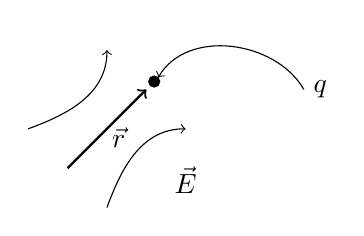
\begin{tikzpicture}
	\draw[thick,->] (0,0) -- (1,1) node[below,xshift=-10pt,yshift=-10pt] {$  \vec{r} $};
	\draw[<-] (1.15,1.15) to[out=60,in=120] (3,1) node[right] {$ q $};
	\draw[fill=black] (1.1,1.1)circle(2pt);
	\draw[->] (-.5,.5) to[out=20,in=-90] (.5,1.5);
	\draw[->] (.5,-.5) to[out=70,in=180] (1.5,.5) node[below,yshift=-10pt] {$ \vec{E} $};
	\end{tikzpicture}
\end{minipage}%
\\
%andrez 1:
\subsection{Elektrostatische Potentielle Energie}

\paragraph{Energie einer Verteilung von Punktladungen}

\begin{minipage}{.6\linewidth}
	$N$ Ladungen $q$: an Orten $\vec{r}_i$\\
	Zunächst: $\underbrace{i - 1}_{\mathclap{\textrm{erzeugen am Ort } \vec{r}_i}}$ Ladungen $q_j$ bei $\vec{r}_j$
\end{minipage}%
\begin{minipage}{.4\linewidth}
	\flushright
	%t1:
	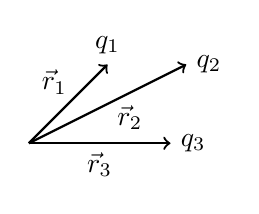
\begin{tikzpicture}
		\draw[thick,->] (0,0) -- (1,1) node[above] {$ q_1 $};
		\draw[thick,->] (0,0) -- (2,1) node[right] {$ q_2 $};
		\draw[thick,->] (0,0) -- (1.8,0) node[right] {$ q_3 $};
		\node[above,xshift=-5pt] at (.5,.5) {$ \vec{r}_1 $};
		\node[right,yshift=-5pt] at (1,.5) {$ \vec{r}_2 $};
		\node[below] at (.9,0) {$ \vec{r}_3 $};
	\end{tikzpicture}
\end{minipage}%
\\
Das Potential
$$\Phi(\vec{r}_i) = \kq \summ{j = 1}{i - 1} \frac{q_i}{|\vec{r}_j - \vec{r}_i|}$$ 
Arbeit um $ i $-te Ladung aus dem unendlichen nach $ \vec{r} $ zu bringen:
\begin{equation*}
W_i = q_i \Phi(\vec{r}_i) = \frac{1}{4 \pi \epsilon_0} \sum_{j=1}^{i-1} \frac{q_i q_j}{r_{ij}}
\end{equation*}
Somit ergibt sich die gesamte Arbeit für $ N $ Ladungen als:
\begin{align*}
W = \sum_{i=2}^{N} W_i &= \frac{1}{4 \pi \epsilon_0} \sum_{i=2}^{N} \sum_{j=1}^{i-1} \frac{q_i q_j}{r_{ij}}\\
&= \kq \frac{1}{2} \sum_{i=1}^{N} \sum_{\substack{j=1 \\ j\neq i}}^{N} \frac{q_i q_j}{r_{ij}}
\end{align*}
\begin{equation*}
\Rightarrow W = \frac{1}{8 \pi \epsilon_0} \sum_{\substack{i,j\\i\neq j}} \frac{q_i q_j}{r_{ij}}
\end{equation*}
% andrez 2:
\begin{align*}
W &= \frac{1}{2} \summ{i = 1}{N} q_i \underbrace{\bigg( \sum_{\substack{j\\ j \neq i}} \kq \frac{q_j}{r_{ij}}\bigg)}_{\Phi_{/ \hspace{-3.5pt}i}(\vec{r}_i)} = \frac{1}{2} \summ{i = 1}{N} q_i \Phi_{/ \hspace{-4pt}i}(\vec{r}_i)
\end{align*}

\paragraph{Energie einer kontinuierlichen lokalisierten Ladungsverteilung}

\begin{minipage}{.3\linewidth}
	%t2:
	\centering
	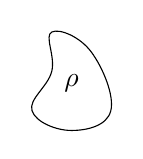
\begin{tikzpicture}
	\draw  plot [smooth cycle, tension=.7] coordinates { (0,0) (.25,.5) (.25,1) (.75,.75) (1,0) (.5,-.25)};
	\node at (.5,.35) {$ \rho $};
	\end{tikzpicture}
\end{minipage}%
\begin{minipage}{.7\linewidth}
	\begin{align*}
	W &= \frac{1}{8 \pi \epsilon_0} \int \dd^3r\ \int \dd^3r'\ \frac{\rho(\vec{r}) \rho(\vec{r}')}{|\vec{r}_j - \vec{r}_i|}\\
	&= \frac{1}{2} \int \dd^3r\ \rho(\vec{r}) \underbrace{ \kq \int_{\mathbb R^3} \dd^3r'\ \frac{\rho(\vec{r}')}{|\vec{r}_j - \vec{r}_i|}}_{\Phi(\vec{r})}
	\end{align*}
\end{minipage}%

\noindent
\begin{minipage}{.3\linewidth}
	%t3:
	\centering
	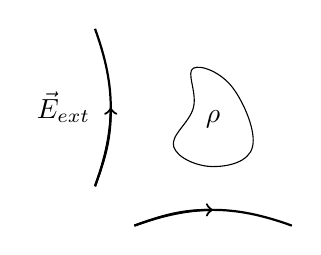
\begin{tikzpicture}
	\draw  plot [smooth cycle, tension=.7] coordinates { (0,0) (.25,.5) (.25,1) (.75,.75) (1,0) (.5,-.25)};
	\node at (.5,.35) {$ \rho $};
	\draw[thick] (-.5,-1) to[out=20,in=160] (1.5,-1);
	\draw[thick] (-1,-.5) to[out=70,in=-70] (-1,1.5);
	\draw[thick,->] (-.5,-1) to[out=20,in=180] (.5,-.8);
	\draw[thick,->] (-1,-.5) to[out=70,in=-90] (-.8,.5);
	\node at (-1.4,.5) {$ \vec{E}_{\tx{ext}} $};
	\end{tikzpicture}
\end{minipage}%
\begin{minipage}{.7\linewidth}
	$$W_{\textrm{ext}} = \int \dd^3 r\ \rho(\vec{r}) \Phi_{\textrm{ext}}(\vec{r})$$
\end{minipage}%

\subsubsection{Energie $ W $ durch $ \vec{E} $ ausdrücken:}

\begin{align*}
\vec\Delta \Phi &= - \frac{1}{\epsilon_0} \rho \quad \Rightarrow \quad W = -\frac{1}{2} \int \dd^3r \epsilon_0 \ub{\vec\Delta \Phi(\vec{r}) \Phi(\vec{r})}_{\vec{\nabla} \cdot (\Phi \vec{\nabla} \Phi) - \equalto{(\vec{\nabla} \Phi)^2}{\vec{E}} }\\
&= -\frac{\epsilon_0}{2} \ub{\int_{\mathbb{R}^3} \dd^3r \vec{\nabla} \cdot (\Phi \vec{\nabla} \Phi)} + \frac{\epsilon_0}{2} \int \dd^3r \vec{E}^2(\vec{r})\\[5pt]
& \qquad \qquad \lim\limits_{R\to \infty} \int_{K_R(0)} \dd^3r \vec{\nabla} \cdot (\Phi \vec{\nabla} \Phi) = \lim\limits_{R \to \infty} \int_{\partial K_R(0)} \ub{\dd\vec{f} \cdot \ub{(\Phi \vec{\nabla}\Phi)}_{\buildrel {R\to \infty} \over \sim \frac{1}{R^3}}}_{\sim \frac{1}{R}} = 0\\
&= \frac{\epsilon_0}{2} \int \dd^3r \vec{E}^2(\vec{r})
\end{align*}
Zur Umformung oben wurde benutzt:
\begin{equation*}
\Phi \buildrel R\to \infty \over \sim \frac{1}{R} \qquad \vec{\nabla} \Phi \sim \frac{1}{R^2}\qquad \dd\vec{f} = \vec{n} \ub{\dd f}_{\sim R^2}
\end{equation*}
Damit ergibt sich für die Energie einer Verteilung von Punktladungen 
% andrez 3:
$$\Rightarrow \quad \rmbox{W = \frac{\epsilon_0}{2} \int \dd^3 r\ \vec{E}^2(\vec{r})} \qquad \textrm{nicht für Punkladungen selbst!!!}$$
\begin{minipage}{.6\linewidth}
	Energiedichte des elektrostatischen Feldes
	$$\rmbox{w(\vec{r}) = \frac{\epsilon_0}{2} \vec{E}^2(\vec{r})}$$
\end{minipage}%
\begin{minipage}{.4\linewidth}
	\flushright
	%t4:
	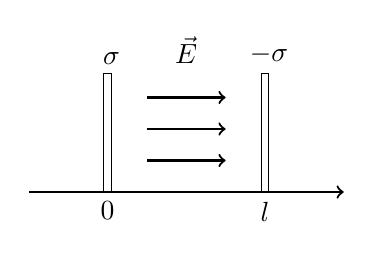
\begin{tikzpicture}
		\draw[thick,->] (-1,0) -- (3,0);
		\draw (-.05,0) rectangle (.05,1.5) node[above] {$ \sigma $};
		\draw (2-.05,0) rectangle (2+.05,1.5) node[above] {$ -\sigma $};
		\node[below] at (0,0) {0};
		\node[below] at (2,0) {$ l $};
		\draw[thick,->] (.5,.4) -- (1.5,.4);
		\draw[thick,->] (.5,.8) -- (1.5,.8);
		\draw[thick,->] (.5,1.2) -- (1.5,1.2);
		\node at (1,1.8) {$ \vec{E} $};
	\end{tikzpicture}
\end{minipage}%

\noindent
\begin{minipage}{.6\linewidth}
	\emph{Beispiel:} \textbf{Plattenkondensator}\\
	Fläche $F$, Ladung $\rightarrow\ \sigma = \frac{q}{F}\ \rightarrow\ \vec{E} = \frac{\sigma}{\epsilon_0} \vec{e}_x$\\[5pt]
	$ \rightarrow $ Die Energiedichte ist: $ w = \frac{\epsilon_0}{2} \vec{E}^2 = \frac{\sigma^2}{2 \epsilon_0} $ (nicht für Punktladungen)\\[5pt]
	$ \rightarrow $ Die Energie beträgt: $ W = \int \dd^3 r w(\vec{r}) = l \cdot F \cdot \frac{\sigma^2}{2 \epsilon_0} $
\end{minipage}%
\begin{minipage}{0.1\linewidth}
	$ \phantom{M} $
\end{minipage}%
\begin{minipage}{.3\linewidth}
	\flushright
	%t5:
	\begin{tikzpicture}
	\draw[->] (-1,0) -- (3,0);
	\node[above] at (0,2)  {$ \phantom{M} $};
	\draw[<-] (0,2) -- (0,-.3) node[below] {0};
	\draw (2,.2) -- (2,-.2) node[below] {$ l $};
	\draw[thick] (-1,0.01) -- (0,0.01);
	\draw[thick] (2,0.01) -- (3,0.01);
	\draw (0,1.2) -- (-.3,1.2) node[left] {$ \frac{\sigma}{\epsilon_0} $};
	\draw[thick] (2,1.2) --(0,1.2);
	\draw[thick] (2,1.21) -- (0,1.21);
	\end{tikzpicture}
\end{minipage}%

\subsubsection{Potentialdifferenz - Spannung}
\begin{equation*}
\Phi(\vec{r}) - \Phi(0) = - \int_{0}^{\vec{r}} \dd\vec{r}' \cdot \vec{E} (\vec{r}') = - \int_{0}^{x} \dd x' \frac{\sigma}{\epsilon_0} = - \frac{\sigma}{\epsilon_0} x
\end{equation*}
%t6: %t7:
$$
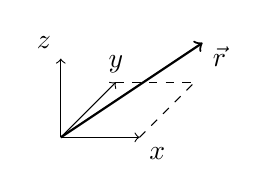
\begin{tikzpicture}
\draw[->] (0,0) -- (0,1) node[anchor=south east] {$ z $};
\draw[->] (0,0) -- (.7,.7) node[anchor=south] {$ y $};
\draw[->] (0,0) -- (1,0) node[anchor=north west] {$ x $};
\draw[dashed] (.7,.7) -- (.7+1,.7);
\draw[dashed] (1,0) -- (1+.7,.7);
\draw[thick,->] (0,0) -- (1.8,1.2) node[right,yshift=-5pt] {$ \vec{r} $};
\end{tikzpicture}
\qquad \qquad 
\begin{tikzpicture}
\draw[->] (-.5,0) -- (1.5,0) node[anchor=north west] {$ x $};
\draw[->] (0,-1) -- (0,1) node[anchor=south east] {$ \Phi $};
\draw[thick] (0,0) -- (1,-1);
\draw[dashed] (1,-1) -- (1,.2) node[anchor=north west,yshift=-5pt] {$ l $};
\end{tikzpicture}
$$
Die Spannung zwischen zwei Kondensatorplatten ist dann:
\begin{equation*}
U = \Phi(0) - \Phi(l) = \frac{\sigma}{\epsilon_0} l = \frac{q}{\epsilon_0 F} l
\end{equation*}
Die Kapazität ist also:
\begin{equation*}
C = \frac{q}{U} = \frac{\epsilon_0 F}{l}
\end{equation*}
% andrez 4:
\lcom{Was ist die Energie bei einer Verteilung von Punktladungen und bei einer kontinuierlichen Ladungsverteilung. Bei einer kontinuierlichen Ladungsverteilung haben wir herausgefunden:}
$$W = \frac{1}{8 \pi \epsilon_0} \sum_{\substack{i,j\\ i \neq j}} \frac{q_i q_j}{r_{ij}} \qquad \textrm{ für Punktladungen}$$
\lcom{Die Energie der Punktladung selbst steckt hier nicht drinnen. Man muss dabei aufpassen, welche Gleichung man für welches Modell benutzt.}
$$\vec{E} = \kq q \frac{\vec{r}}{r^3} \qquad \int \dd^3 r\ \vec{E}^2 = \int \dd^3 r\ \frac{1}{r^4} = \infty$$

\section{Verhalten des el. Feldes an Grenzflächen mit Flächenladung}
$ \rightarrow $ Diskontinuitäten von $ \vec{E} $\\
\emph{Beispiel:} Wir betrachten eine\textbf{ homogene Flächenladung}.\\[10pt]
\begin{minipage}{.4\linewidth}
	%t8: %t9: %t10: %t11:
	\begin{tikzpicture}
	\draw (-1,-1) to[out=45,in=180] (1.2,0);
	\draw (-1.2,-.4) to[out=45,in=180] (1,.6);
	\draw (-.8,-1.6) to[out=45,in=180] (1.4,-.6);
	\draw (0,1) to[out=-30,in=90] (1,-1);
	\draw (-.7,.7) to[out=-30,in=90] (.3,-1.3);
	\draw (-1.4,.2) to[out=-30,in=90] (-.4,-1.6);
	\draw[thick,<-] (.5,.3) to[out=60,in=180] (1.5,1) node[right] {$ \sigma(\vec{r}) = \frac{\tx{Ladung}}{\tx{Fläche}} $};
	\end{tikzpicture}
\end{minipage}%
\begin{minipage}{.3\linewidth}
	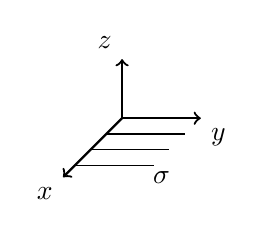
\begin{tikzpicture}
	\draw[thick,->] (0,0) -- (0,.75) node[anchor=south east] {$ z $};
	\draw[thick,->] (0,0) -- (1,0) node[anchor=north west] {$ y $};
	\draw[thick,->] (0,0) -- (-.75,-.75) node[anchor=north east] {$ x $};
	\draw (-.2,-.2) -- (-.2+1,-.2);
	\draw (-.4,-.4) -- (-.4+1,-.4);
	\draw (-.6,-.6) -- (-.6+1,-.6);
	\node at (.5,-.75) {$ \sigma $};
	\end{tikzpicture}
\end{minipage}\nolinebreak%
\begin{minipage}{.3\linewidth}
	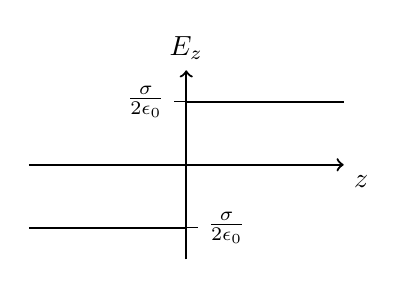
\begin{tikzpicture}
	\draw[thick,->] (0,-1.2) -- (0,1.2) node[above] {$ E_z $};
	\draw[thick,->] (-2,0) -- (2,0) node[anchor=north west] {$ z $};
	\draw[thick] (2,.8) -- (0,.8) ;
	\draw (0,.8) -- (-.15,.8) node[left] {$ \frac{\sigma}{2 \epsilon_0} $};
	\draw[thick] (-2,-.8) -- (0,-.8);
	\draw (0,-.8) -- (.15,-.8) node[right] {$\frac{\sigma}{2 \epsilon_0}$};
	\end{tikzpicture}
\end{minipage}%
\begin{equation*}
\Rightarrow \vec{E} = \frac{\sigma}{2 \epsilon_0} \tx{sgn}(z) \vec{e}_z
\end{equation*}
\begin{align*}
\vec{E}_\perp &= \pm \frac{\sigma}{2 \epsilon_0} \vec{e}_z\\
\vec{E}_\parallel &= 0
\end{align*}
\begin{minipage}{.6\linewidth}
	Das elektrische Feld $ \vec{E}_\parallel $ ist gleich der Ableitung des elektrischen Potentials:\\
	Das elektrische Potential ist also stetig.
\end{minipage}%
\begin{minipage}{.4\linewidth}
	\hspace{30pt}
	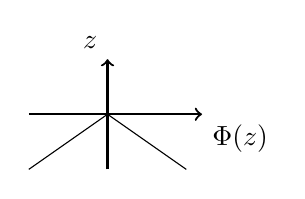
\begin{tikzpicture}
	\draw[thick,->] (0,-.7) -- (0,.7) node[anchor=south east] {$ z $};
	\draw[thick,->] (-1,0) -- (1.2,0) node[anchor=north west] {$ \Phi(z) $};
	\draw (-1,-.7) -- (0,0) -- (1,-.7);
	\end{tikzpicture}
	\vspace{5pt}
\end{minipage}%

\noindent
\begin{minipage}{.4\linewidth}
	%andrez 5:
	
	\paragraph{Normalkomponente $\vec{E}_\perp$}
	
	Gaußscher Satz für $V$:
	\vspace{50pt}
\end{minipage}%
\begin{minipage}{.6\linewidth}
	%t12:
	\centering
	\begin{tikzpicture}[scale=.8]
	\coordinate (o) at (0,0);
	\coordinate (O) at (-4,-2);
	\draw[fill=gray!7.5] (-3,-1.4) -- (1.5,-1.4) -- (3,1.4) -- (-1.5,1.4) -- (-3,-1.4);
	\draw[->] (O) -- ++(.4,0);
	\draw[->] (O) -- ++(0,.4);
	\draw[->] (O) -- ++(.3,.3);
	\draw[red,fill=red!5] (o) ellipse (1cm and .5cm);
	\draw[red,fill=red!5] ($ (o) + (0,2) $) ellipse (1cm and .5cm);
	\draw[red,dashed,fill=red!5] ($ (o) + (0,-2) $) ellipse (1cm and .5cm);
	\draw[red] (-1,2) -- (-1,0);
	\draw[red] (1,2) -- (1,0);
	\draw[red,dashed] (-1,-2) -- (-1,0);
	\draw[red,dashed] (1,-2) -- (1,0);
	\draw[red,thick,->] (o) -- ++(0,3) node[anchor=west] {$ \vec{n}_+ $};
	\draw[blue,thick,->] (o) -- ++(0,-3) node[anchor=east] {$ \vec{n}_- $};
	\draw[thick,->] (O) -- (o) node[xshift=-70pt,yshift=-20pt] {$ \vec{r} $};
	\node[right] at (o) {$ F $};
	\node[anchor=north west] at ($ (o) + (0,1.2) $) {$ \partial V_+ $};
	\node[anchor=north west] at ($ (o) + (0,-.8) $) {$ \partial V_- $};
	\draw[decorate, decoration={brace,amplitude=10pt,mirror,raise=2pt}, xshift=-10pt,red]  (-1,2) -- node[left=20pt] {$\Delta z$}  (-1,-2);
	\node at (2.2,1) {$ \sigma(\vec{r}) $};
	\draw ($ (o) + (.5,.3) $) to[out=30,in=150] (2.7,0) node[right] {$ V = \Delta z \cdot F $};
	\node[circle,fill=blue,inner sep=1pt,minimum size=1pt] at (0,-2) {};
	\node[circle,fill=red,inner sep=1pt,minimum size=1pt] at (0,2) {};
	\end{tikzpicture}
\end{minipage}%
\vspace{-10pt}
\begin{align*}
\int_V \dd^3 r'\ \vabla \cdot \vec{E}(\vec{r'}) &= \int_{\partial V} \dd\vec{f}'\ \vec{E}(\vec{r})\\
&=\custo{\overset{\rotatebox{90}{$\scriptscriptstyle{\Delta z \to 0}$}}{\longrightarrow}}{\int_{\textrm{Mantel}} \dd\vec{f}'\ \vec{E}}{\hspace{-23.5pt}0} + \custo{\overset{\rotatebox{90}{$\scriptscriptstyle{\Delta z \to 0}$}}{\longrightarrow}}{\int_{\partial V_+} \dd\vec{f}'\ \vec{E}(\vec{r})}{\int_F \dd f'\ \vec{n} \cdot \vec{E}_+} + \custo{\overset{\rotatebox{90}{$\scriptscriptstyle{\Delta z \to 0}$}}{\longrightarrow}}{\int_{\partial V_-} \dd\vec{f}'\ \vec{E}}{- \int_F \dd f'\ \vec{n} \cdot \vec{E}_-}
\end{align*}
$ \vec{E}_{\pm} $ ist das Feld auf beiden Seiten der Grenzfläche
% eaualto zwischen Zeile 1 und 2 der equations ...
\begin{equation*}
\int_{\partial V} \dd\vec{f}' \vec{E} \quad \buildrel \Delta z \to 0 \over \longrightarrow \quad \int_{F} \dd f \vec{n} \cdot (\vec{E}_+ - \vec{E}_-) \quad \buildrel F \to 0 \over \longrightarrow \quad F \ \vec{n} \cdot \big(\vec{E}_+(\vec{r}) - \equalto{\vec{E}_-(\vec{r})}{}\big)
\end{equation*}
\begin{equation*}
\int_V \dd^3r' \equalto{\vec{\nabla} \cdot \vec{E}(\vec{r}')}{\frac{1}{\epsilon_0} \rho(\vec{r}')} = \frac{1}{\epsilon_0} \int_V \dd^3r' \rho(\vec{r}) = \frac{1}{\epsilon_0} \int_F \dd f'  \sigma(\vec{r}') \quad \buildrel F \to 0 \over \longrightarrow \quad \frac{1}{\epsilon_0} F \sigma(\vec{r})
\end{equation*}
\begin{equation*}
\Rightarrow \vec{n} \cdot \left(\vec{E}_+(\vec{r}) - \vec{E}_-(\vec{r}) \right) = \frac{1}{\epsilon_0} \sigma(\vec{r})
\end{equation*}
\begin{equation*}
E_{\perp_\pm} = \vec{n} \cdot \vec{E}_{\pm} \qquad E_{\perp_+}(\vec{r}) - E_{\perp_-} (\vec{r}) = \frac{1}{\epsilon_0} \sigma(\vec{r})
\end{equation*}

%t13: und Tafel vor M4:
\noindent
\begin{minipage}{.4\linewidth}
	
	\paragraph{Tangentialkomponente $ E_\parallel $}
	
	Satz von Stokes:
	\vspace{50pt}
\end{minipage}%
\begin{minipage}{.6\linewidth}
	\centering
	\begin{tikzpicture}[scale=1.15]
		\draw (-2,1) to[out=-10,in=135] (0,0) to[out=-45,in=100] (1,-2);
		%\draw (-.3,1.25) -- (1.25,.3) -- (.3,-1.25) -- (-1.25,-.3) -- (-.3,1.25);
		\draw[->] ($ (0,0) + (-.25,1.25) + (-45:2cm) + (-135:1.5cm) $) -- ($ (0,0) + (-.25,1.25) + (-45:2cm) + (-135:.6cm) $);
		\draw[->] ($ (0,0) + (-.25,1.25) + (-45:2cm) $) -- ($ (0,0) + (-.25,1.25) + (-45:1cm) $);
		\draw[->] ($ (0,0) + (-.25,1.25) $) -- ($ (0,0) + (-.25,1.25) + (-135:.75cm) $);
		\draw[->] ($ (0,0) + (-.25,1.25) + (-135:1.5cm) $) -- ($ (0,0) + (-.25,1.25) + (-135:1.5cm) + (-45:1cm) $);
		\draw[draw=none,fill=gray,opacity=.1] ($ (0,0) + (-.25,1.25) $) -- ++(-135:1.5cm) -- ++(-45:2cm) -- ++(45:1.5cm) -- ++(135:2cm);
		\draw ($ (0,0) + (-.25,1.25) $) -- ++(-135:1.5cm) -- ++(-45:2cm) -- ++(45:1.5cm) -- ++(135:2cm);
		\draw[decorate, decoration={brace,amplitude=10pt,raise=2pt},red] ($ (0,0) + (-.25,1.25) $) -- node[above=10pt,xshift=13pt] {$ L $} ($ (0,0) + (-.25,1.25) + (-45:2cm) $);
		\draw[decorate, decoration={brace,amplitude=10pt,mirror,raise=2pt},red] ($ (0,0) + (-.25,1.25) $) -- node[above=10pt,xshift=-12pt] {$ \Delta z $} ($ (0,0) + (-.25,1.25) + (-135:1.5cm) $);
		\node at (1,-1) {$ \gamma $};
		\coordinate (O) at (-1.5,-1.5);
		\draw[->] (O) -- ++(.4,0);
		\draw[->] (O) -- ++(0,.4);
		\draw[->] (O) -- ++(.25,.25);
		\node[anchor=north east] at (O) {$ O $};
		\draw[thick,->] (O) -- (0,0) node[anchor=north east,yshift=-15pt,xshift=-25pt] {$ \vec{r} $};
		\draw[thick,->] (0,0) -- ++(135:.75cm) node[anchor=south west,yshift=-10pt,xshift=5pt] {$ \vec{E} $};
		\node at (-2,.3) {$ \sigma $};
	\end{tikzpicture}
\end{minipage}%
\begin{equation*}
0 = \oint_r \dd\vec{r} \vec{E}(\vec{r}') = \ub{
	\int\limits_{\begin{tikzpicture}[scale=.7]
		\draw[dashed] (0,0) -- (1,0) -- (1,.7) -- (0,.7) -- (0,0);
		\draw[thick,->] (1,0) -- (1,.7);
		\end{tikzpicture}} \dots + 
	\int\limits_{\begin{tikzpicture}[scale=.7]
		\draw[dashed] (0,0) -- (1,0) -- (1,.7) -- (0,.7) -- (0,0);
		\draw[thick,->] (0,0) -- (0,.7);
		\end{tikzpicture}} \dots}_{= 0 \tx{ für } \Delta z \to 0} + \ub{
	\int\limits_{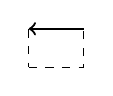
\begin{tikzpicture}[scale=.7]
		\draw[dashed] (0,0) -- (1,0) -- (1,.7) -- (0,.7) -- (0,0);
		\draw[thick,->] (1,.7) -- (0,.7);
		\end{tikzpicture}} d\vec{r}' \vec{E} + 
	\int\limits_{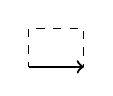
\begin{tikzpicture}[scale=.7]
		\draw[dashed] (0,0) -- (1,0) -- (1,.7) -- (0,.7) -- (0,0);
		\draw[thick,->] (0,0) -- (1,0);
		\end{tikzpicture}} d\vec{r}' \vec{E} }_{
	\int\limits_{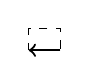
\begin{tikzpicture}[scale=.4]
		\draw[dashed] (0,0) -- (1,0) -- (1,.7) -- (0,.7) -- (0,0);
		\draw[thick,->] (1,0) -- (0,0);
		\end{tikzpicture}} \dd\vec{r}' (\vec{E}_+ -  \vec{E}_-)}
\end{equation*}
\begin{equation*}
0 = \oint_\gamma \dd\vec{r}' \cdot \vec{E} \quad \buildrel \Delta z \to 0 \over \longrightarrow \quad \int_{-\frac{L}{2}}^{-\frac{L}{2}} \dd s \vec{t} \cdot \left(\vec{E}_+ - \vec{E}_-\right) \quad \buildrel L \to 0 \over \longrightarrow \quad L \ \vec{t} \cdot \left(\vec{E}_+(\vec{r}) - \vec{E}_-(\vec{r})\right) = 0
\end{equation*}
\begin{equation*}
\rightarrow \vec{t} \cdot (\vec{E}_+ (\vec{r}) - \vec{E}_- (\vec{r})) = 0
\end{equation*}
$\rightarrow $ Die Tangentialkomponente ist stetig
\begin{equation*}
E_{\parallel_{+}} = E_{\parallel_{-}}
\end{equation*}
Insgesamt ergibt sich damit:
\begin{equation*}
\vec{E}_+(\vec{r}) - \vec{E}_-(\vec{r}) = \frac{\sigma}{\epsilon_0} \vec{n}
\end{equation*}
\begin{minipage}{.6\linewidth}
	Das elektrische Potential $ \Phi $ ist damit stetig.
	\begin{equation*}
	\ub{\Phi(\vec{r}_b) - \Phi(\vec{r}_a)}_{\Phi_+(\vec{r}) - \Phi_-(\vec{r})} = \int_{\vec{r}_a}^{\vec{r}_b} \dd\vec{r}' \cdot \vec{E} \quad \buildrel \Delta z \to 0 \over \longrightarrow 0
	\end{equation*}
	Und hiermit auch auf beiden Seiten der Flächenladung symmetrisch.
\end{minipage}%
\begin{minipage}{.4\linewidth}
	%t14:
	\centering
	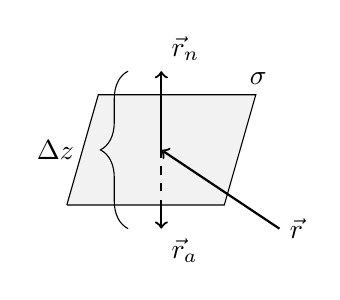
\begin{tikzpicture}
		\draw[fill=gray!10] (-1.2,-.7) -- (.8,-.7) -- (1.2,.7) -- (-.8,.7) -- (-1.2,-.7);
		\draw[thick,<-] (0,0) -- (1.5,-1) node[anchor=west] {$ \vec{r} $};
		\node[anchor=south west] at (1,.7) {$ \sigma $};
		\draw[thick,->] (0,0) -- (0,1) node[anchor=south west] {$ \vec{r}_n $};
		\draw[thick,dashed] (0,0) -- (0,-.7);
		\draw[thick,->] (0,-.7) -- (0,-1) node[anchor=north west] {$ \vec{r}_a $};
		%\draw[decorate, decoration={brace,amplitude=10pt,raise=2pt},red] ($ (0,0) + (-.25,1.25) $) -- node[above=10pt,xshift=13pt] {$ L $} ($ (0,0) + (-.25,1.25) + (-45:2cm) $);
		\draw[decorate, decoration={brace,amplitude=10pt,mirror,raise=2pt+10pt}] (0,1) -- node[left,xshift=-28pt] {$ \Delta z $} (0,-1);
	\end{tikzpicture}
\end{minipage}%

% andrez 6 oder 5:
\subsection{Randbedingungen an el. Leitern}

\begin{minipage}{.6\linewidth}
	Leiter: Material mit freibeweglichen Ladungsträgern (Metall)\\
	Eigenschaften von $\vec{E}$ im Leiter:
\end{minipage}%
\begin{minipage}{.4\linewidth}
	%t15:
	\centering
	\begin{tikzpicture}
		\draw[thick] (0,0) arc (90:0:2.5cm);
		\draw[draw=none,pattern=north east lines] (0,0) arc (90:0:2.5cm) -- ++(-2.5,0) -- (0,0);
		\node[right] at (1.5,0) {Vakuum};
		\node[fill=white,opacity=.8,rounded corners] at (1,-2) {Leiter};
		\node[fill=white,opacity=.8,rounded corners] at (1,-1) {$ \vec{E} = 0 $};
	\end{tikzpicture}
\end{minipage}%
\\[10pt]
\begin{minipage}{.6\linewidth}
	\begin{enumerate}[i)]
		\item $\vec{E} = 0$
		\item $0 = \vabla \cdot \vec{E} = \frac{1}{\epsilon_0} \rho, \qquad \rho(\vec{r}) = 0$
		\item Nettoladung befinden sich an Oberfläche %t16
		\item Potential $\Phi(\vec{r}_b) - \Phi(\vec{r}_a) = 0 \quad \rightarrow \quad \Phi(\vec{r}) = \const$ % t17
	\end{enumerate}
\end{minipage}%
\begin{minipage}{.4\linewidth}
		%t16:
		\centering
		\begin{tikzpicture}[scale=.8]
		\draw[pattern=north east lines] (0,0) circle (1cm);
		\draw[fill=white,opacity=.6,draw=none] (0,0) circle (.995cm);
		\foreach \x/\xtext in {0/$+$,45/$+$,90/$+$,135/$+$,180/$+$,225/$+$,270/$+$,315/$+$}
		\node at (\x:.8cm) {\xtext};
		\draw[<-] (-45:1.2cm) -- ++(.5,-.2) node[right] {$ \substack{\tx{Flächenladung} \\ \sigma} $};
		\end{tikzpicture}\\
		%t17:
		\begin{tikzpicture}[scale=.8]
		\draw[pattern=north east lines] (0,0) circle (1cm);
		\draw[fill=white,opacity=.7,draw=none] (0,0) circle (.995cm);
		\node[circle,fill=black,inner sep=1pt,minimum size=1pt] (b) at (-.7,.25) {};
		\node[circle,fill=black,inner sep=1pt,minimum size=1pt] (a) at (.7,.25) {};
		\draw (a) --(b);
		\node[below] at (a) {$ \vec{r_a} $};
		\node[below] at (b) {$ \vec{r_b} $};
		\end{tikzpicture}\hspace{66pt}
\end{minipage}%

\paragraph{Randbedingungen}
%
%
%
% I27 T18
%
%
%
$$\vec{E}_+ - \vec{E}_- = \frac{\sigma^-}{\epsilon_0} \vec{n}$$
$$\vec{E}_- = 0$$
$$\rightarrow \vec{E}_+(\vec{r}) = \frac{\sigma(\vec{r})}{\epsilon_0} \vec{n} {(\vec{r})}$$
\folie{Ladung an Oberfläche eines Leiters}


% 5.11.18

\section{Randwertprobleme (RWP) der Elektrostatik und \texorpdfstring{\\}{newline} Lösungsmethoden}

\subsection{Formulierung des Randwertproblems}

Das elektrische Potential: $ \Phi(\vec{r}): \quad \vec{E}(\vec{r}) = - \vec{\nabla} \Phi(\vec{r}) $\\
$$ \vec{\Delta} \Phi (\vec{r}) = -\frac{1}{\epsilon_0} \rho(\vec{r})  \qquad \tx{Poisson-Gleichung}$$
Für eine gegebene lokale Ladungsverteilung $ \rho $ gilt:
\begin{equation*}
\Phi(\vec{r}) = \frac{1}{4 \pi \epsilon_0} \int \dd^3 r' \frac{\rho(\vec{r}')}{|\vec{r} - \vec{r}'|}
\end{equation*}
%
%
%
% I28 evtl |r| gegen 0 aber |r| gegen unendlich macht mehr sinn
%
%
%
\begin{equation*}
\rightarrow \Phi(\vec{r}) \buildrel |\vec{r}| \rightarrow \infty \over \longrightarrow 0
\end{equation*}
Typische Problemstellung:\\
Ladungsverteilung $\rho$ + Werte des Potentials auf Randfläche\\[5pt]
\bei\\
\begin{minipage}{.6\linewidth}
	Randwertproblem: Gegeben: $\rho(\vec{r}')$ im Raumbereich $V$\\
	$\Phi(\vec{r})$ oder $\vec{E}(\vec{r})$ auf Randfläche $\partial V$\\
	Gesucht: $\Phi(\vec{r}),\ \vec{E}(\vec{r})$ überall in $V$
\end{minipage}%
\begin{minipage}{.4\linewidth}
	%t1:
	\centering
	\begin{tikzpicture}
		\draw[pattern=north east lines] (0,0) circle (.7cm);
		\draw[thick] (-.7,0) -- ++(-.5,0) -- ++(0,-1);
		\coordinate (e) at (-1.2,-1);
		\draw[thick] ($ (e) + (-.25,0) $) -- ++(.5,0);
		\draw[thick] ($ (e) + (-.125,0) + (0,-.1) $) -- ++(.25,0);
		\draw[thick] ($ (e) + (-.0625,0) + (0,-.2) $) -- ++(.125,0);
		\draw (.25,.15) to[out=55,in=190] (1.2,.8) node[right] {$ \Phi = 0 $};
		\node[fill=black,circle,inner sep=1pt,minimum size=1pt] (q) at (1.5,0) {};
		\node[right] at (q) {$ q $};
	\end{tikzpicture}
\end{minipage}%
\\
Zwei Fälle:
\begin{enumerate}[i)]
	\item $ \Phi(\vec{r}) $ ist auf der Randfläche gegeben\\
	$ \rightarrow $ \textbf{Dirichlet-Randbedingung}
	\item $ \vec{E}(\vec{r}) $ ist auf der Randfläche gegeben\\
	$ \rightarrow $ \textbf{Neumannsche Randbedingung}
\end{enumerate}
\noindent
\begin{minipage}{.6\linewidth}
	Gegeben sei: $ \vec{n} \cdot \vec{E} $ dies ist gleich der \textbf{Normalenableitung}:
	\begin{equation*}
	\vec{n} \cdot \vec{E} = - \vec{n} \vabla \Phi = - \prt{\Phi}{n}
	\end{equation*}
\end{minipage}%
\begin{minipage}{.4\linewidth}
	%t2:
	\centering
	\begin{tikzpicture}[scale=.8]
		\draw[draw=none,pattern=north east lines] (0,0) -- (120:1.5cm) arc (120:-20:1.5cm) -- (0,0);
		\draw ($ (0,0) + (120:1.5cm)$) arc (120:-20:1.5cm);
		\draw[thick,->] ($ (50:1.5cm) $) -- ++(50:1cm) node[xshift=-15pt,yshift=-5pt] {$ \vec{n} $};
	\end{tikzpicture}
	\vspace{5pt}
\end{minipage}%
\\
\lcom{Wir beschränken uns vorwiegend auf den ersten Fall. }
\lcom{Zur Lösung dieser Probleme gibt es einige Methoden. Zum Einstieg und zur  betrachten wir zunächst die Methode der Spiegelladung. }

\subsection{Methode der Bildladung (Spiegelladung)}

\subsubsection{Punktladung vor leitender, geerdeter Metallplatte}

\begin{minipage}{.6\linewidth}
	\begin{equation*}
	\vec{\Delta} \Phi(\vec{r}) = - \frac{1}{\epsilon_0} \rho (\vec{r}) = - \frac{q}{\epsilon_0} \delta(\vec{r} - \vec{r}_0)
	\end{equation*}
	$ \vec{r} \in V  \qquad \vec{r}_0 = (d,0,0) \qquad V = \{\vec{r} \in \mathbb{R}^3 , x > 0\}$\\[5pt]
	Randbedingungen:
	\begin{equation*}
	\pofr = 0 \quad \tx{für} \quad \vec{r} \in \partial V ,\quad \quad \tx{d.h.} \ \vec{r} = (0,y,z)
	\end{equation*}
\end{minipage}%
\begin{minipage}{.4\linewidth}
	%t3:
	\centering
	\begin{tikzpicture}
		\draw[thick,->] (-.7,0) -- (2,0) node[anchor=north west] {$ x $};
		\draw ($ (-.1,0) + (0,-1.5) $) -- ++(0,3);
		\draw ($ (.1,0) + (0,-1.5) $) -- ++(0,3);
		\draw[draw=none,pattern=north east lines] ($ (-.1,0) + (0,-1.5)  $) rectangle ($ (.1,0) + (0,1.5) $);
		\draw[thick] (0,-.1) -- (0,.1) node[anchor=north east] {$ 0 $};
		\node[fill=black,circle,inner sep=1pt,minimum size=1pt] (q) at (1.5,0) {};
		\node[above] at (q) {$ q $};
		\draw[decorate, decoration={brace,amplitude=5pt,mirror,raise=2pt}, yshift=-4pt,black] (0,0) -- node[below=10pt] {$ d $} (1.5,0);
		\coordinate (e) at (-1,-1.5);
		\draw[thick] (e) -- ++(0,.7) -- ++(.9,0);
		\draw[thick] ($ (e) + (-.25,0) $) -- ++(.5,0);
		\draw[thick] ($ (e) + (-.125,0) + (0,-.1) $) -- ++(.25,0);
		\draw[thick] ($ (e) + (-.0625,0) + (0,-.2) $) -- ++(.125,0);
		\draw (0,.5) to[out=120,in=10] (-1.2,.8) node[left] {$ \Phi = 0 $};
		\node at (1.8,1.2) {$ V \ \ \Phi(\vec{r}) = \ ? $};
	\end{tikzpicture}
	\vspace{10pt}
\end{minipage}%
\\
\textbf{Idee:} Ersetze ursprüngliche Problem durch ,,Fiktives`` Problem mit zusätzlichen Ladungen außerhalb von $V$, welche die Randbedingungen simulieren.\\[5pt]
Potential der Punkladungen in $\vec{r}_0$:
$$\Phi_q (\vec{r}) = \kq \frac{q}{|\vec{r} - \vec{r}_0|}$$
\noindent
\begin{minipage}{.5\linewidth}
	addiere Ladung $-q$ in $\vec{r}'_0 = (-d, 0, 0) = -\vec{r}_0$\\[5pt]
	\begin{equation*}
	\pofr = \kq \left( \frac{q}{|\vec{r} - \vec{r}_0|} - \frac{q}{|\vec{r}+\vec{r}_0|} \right)
	\end{equation*}
\end{minipage}%
\begin{minipage}{.5\linewidth}
	%t4:
	\centering
	\begin{tikzpicture}
		\draw[->] (-2,0) -- (2,0) node[anchor=north west] {$ x $};
		\draw[->] (0,-1) -- (0,1) node[anchor=south east] {$ y $};
		\coordinate (q) at (1.5,0);
		\coordinate (-q) at (-1.5,0);
		\node[circle,fill=black,inner sep=1pt,minimum size=1pt] at (-q) {};
		\node[circle,fill=black,inner sep=1pt,minimum size=1pt] at (q) {};
		\node[above] at (-q) {$ -q $};
		\node[above] at (q) {$ q $};
		\draw[decorate,decoration={brace,amplitude=5pt,raise=2pt},yshift=-4pt,black] (0,0) -- node[below=10pt] {$ d $} (-1.5,0);
		\draw[decorate,decoration={brace,amplitude=5pt,mirror,raise=2pt},yshift=-4pt,black] (0,0) -- node[below=10pt] {$ d $} (1.5,0);
	\end{tikzpicture}
\end{minipage}%
\\
Schauen wir nun nach, ob dies die Poisson-Gleichung erfüllt:
\begin{align*}
\vec{\Delta} \Phi &= \frac{q}{4 \pi \epsilon_0} \Bigg( \ub{\Delta \frac{1}{|\vec{r} - \vec{r}_0|}}_{= - 4 \pi \delta(\vec{r} - \vec{r}_0)} - \ub{\Delta \frac{1}{|\vec{r} + \vec{r}_0|}}_{= - 4 \pi \delta(\vec{r} + \vec{r}_0)}\Bigg)\\
&= \underset{\checkmark}{- \frac{q}{\epsilon_0} \delta(\vec{r} - \vec{r}_0)} + \frac{q}{\epsilon_0} \ub{\delta(\vec{r} + \vec{r}_0)}_{\mathclap{\qquad = 0 \ \tx{für} \ \vec{r} \neq - \vec{r}_0 \ \checkmark \quad \forall \vec{r} \in V}}
\end{align*}

\subsubsection{Diskussion der Lösung}
\begin{enumerate}[i)]
	\item \textbf{Struktur}
	$$\pofr = \underbrace{\frac{q}{4 \pi \epsilon_0} \frac{1}{|\vec{r}-\vec{r}_0|}}_{\eqdef\ \Phi_{\textrm{s}}(\vec{r})} + \underbrace{\frac{(-q)}{4 \pi \epsilon_0} \frac{1}{|\vec{r}+\vec{r}_0|}}_{\eqdef\ \Phi_{\textrm{hom}}(\vec{r})}$$ 
	$ \vec{r} \in V $
	\begin{equation*}
	\Delta \Phi_\tx{s}(\vec{r}) = - \frac{1}{\epsilon_0} \rho(\vec{r}) \quad \tx{Poisson-Gleichung}
	\end{equation*}
	\begin{equation*}
	\Delta \Phi_{\tx{hom}} (\vec{r}) = 0 \qquad \tx{Laplace-Gleichung}
	\end{equation*}
	Mathematisch: Lösung inhomogener DGL
	\begin{equation*}
	\pofr = \Phi_\tx{s}(\vec{r}) + \Phi_{\tx{hom}}(\vec{r})
	\end{equation*}
	$ \Phi_{\tx{hom}} $ wird so gewählt, dass die Randbedingungen erfüllt werden:
	\begin{equation*}
	\vec{r} \in \partial V: \quad \Phi_\tx{o} (\vec{r}) = \Phi_\tx{s}(\vec{r}) + \Phi_{\tx{hom}}(\vec{r})
	\end{equation*}	
	\item \textbf{Elektrisches Feld}
	\begin{equation*}
	\vec{E} = - \vec{\nabla} \Phi = \frac{q}{4 \pi \epsilon_0} \left(\frac{(x-d,y,z)}{|\vec{r} - \vec{r}_0|^3} - \frac{(x+d,y,z)}{|\vec{r} + \vec{r}_0|^3}\right)
	\end{equation*}
	An der Oberfläche $ x \to 0 $, $ x \ge 0 $\\
	$ |\vec{r} \pm \vec{r}_0|^3 \rightarrow (d^2 + y^2 + z^2) $\\
	\begin{minipage}{.5\linewidth}
		\begin{equation*}
		\eofr \bigg|_{\vec{r} \in \partial V} = - \frac{qd}{2 \pi \epsilon_0} \frac{1}{(d^2 + y^2 + z^2) ^{3/2}} \vec{e}_x
		\end{equation*}
		\lcom{Durch das externe elektrische Feld verschieben sich die Ladungsträger im Metall und es entsteht eine Influenzladung an der Oberfläche.}
	\end{minipage}%
	\begin{minipage}{.5\linewidth}
		\centering
		%t5: \draw  plot [smooth cycle, tension=1] coordinates { (0,0) (.5,1.5) (.5,2.5) (2,2) (3,2) (2.5,1) (1.5,0) };
		\begin{tikzpicture}
			\draw[->] (-.5,0) -- (2.5,0) node[anchor=north west] {$ x $};
			\coordinate (q) at (1.5,0);
			\node[circle,fill=black,inner sep=1pt,minimum size=2pt] at (q) {};
			\node[yshift=15pt,xshift=30pt] at (q) {$ q > 0 $};
			\draw[->] (0,-2) -- (0,2) node[anchor=south west] {$ z $};
			\draw[draw=none,pattern=north west lines] (-.3,1.5) node[above,xshift=-5pt] {$ \sigma(z) $} rectangle (0,-1.5);
			\draw[thick,->] (q) to[out=180,in=0] (0,0);
			\draw[thick,->] (q) to[out=155,in=0] (0,.20);
			\draw[thick,->] (q) to[out=90,in=0] (0,.50);
			\draw[thick,->,looseness=1.3] (q) to[out=65,in=0] (0,.85);
			\draw[thick,->,looseness=1.6] (q) to[out=45,in=0] (0,1.3);
			\draw[thick,->,looseness=1.3] (q) to[out=25,in=-45] ($ (q) + (.4,1) $);
			\draw[thick,->] (q) to[out=-155,in=0] (0,-.20);
			\draw[thick,->] (q) to[out=-90,in=0] (0,-.50);
			\draw[thick,->,looseness=1.3] (q) to[out=-65,in=0] (0,-.85);
			\draw[thick,->,looseness=1.6] (q) to[out=-45,in=0] (0,-1.3);
			\draw[thick,->,looseness=1.3] (q) to[out=-25,in=45] ($ (q) + (.4,-1) $);
			\coordinate (n) at (-.5,0);
			\node[rounded corners,align=center,left] at (n) {$ \vec{E}_{\parallel} = 0 $ \\ \\ $ \vec{E}_{\perp} \neq 0 $};
		\end{tikzpicture}
	\end{minipage}%
	\item \textbf{Influenzladung auf Metalloberfläche}
	$$\vec{E}_+ - \equalto{\vec{E}_-}{0} = \frac{\sigma}{\epsilon_0} \vec{n} \qquad \vec{n} = \vec{e}_x$$
	$\vec{r} \in \partial V$:
	$$\sigma (\vec{r}) = \epsilon_0 \vec{E}_+(\vec{r}) = - \frac{qd}{2 \pi(d^2 + y^2 + z^2)^{\nicefrac{3}{2}}}$$
	gesamte influenzierte Ladung
	$$q_i = \int_{\partial V} \dd f\ \sigma(\vec{r}) = \dots = -q$$
	\item \textbf{Kraft zwischen Punktladungen und Metallplatte}
	$$\vec{F} = q \vec{\tilde{E}}(\vec{r}_0) = \frac{-q^2}{4 \pi \epsilon_0 (2d)^2}\vec{e}_x$$
\end{enumerate}

% andrez 5:
\subsubsection{Eindeutigkeit der Lösung des Randwertproblems}

\begin{minipage}{.6\linewidth}
	\textbf{Dirichlet-Randwertproblem:}
	\begin{align*}
	\Delta \pofr = -\frac{1}{\epsilon_0} \rho(\vec{r}) &\qquad \vec{r} \in V\\
	\pofr = \Phi_0 (\vec{r}) \quad \; &\qquad \vec{r} \in \partial V \quad \;
	\end{align*}
\end{minipage}%
\begin{minipage}{.4\linewidth}
	\centering
	\begin{tikzpicture}
		\draw (0,1) -- (0,-1);
		\draw[draw = none,pattern = north east lines] (-.3,1) rectangle (0,-1);
		\node[fill=black,circle,inner sep=1pt,minimum size=1pt] (p) at (-.1,0) {};
		\node[fill=black,circle,inner sep=1pt,minimum size=1pt] (q) at (1,0) {};
		\node[right] at (q) {$ q $};
		\node at (1,.5) {$ V $};
		\node at (0,1.3) {$ \partial V $};
		\draw[thick] (p) to[out=135,in=-10] (-.5,.3) node[left] {$ \Phi_0 $};
	\end{tikzpicture}
\end{minipage}%
\\
Annahme: $\Phi_1,\ \Phi_2$ lösen RWP
\begin{align*}
\textrm{d.h. }\qquad \Delta\Phi_1(\vec{r}) = -\frac{1}{\epsilon_0} \rho(\vec{r}) = \Delta \Phi_2 (\vec{r}) &\qquad \vec{r} \in V\\
\Phi_1 (\vec{r}) = \Phi_0(\vec{r}) = \Phi_2(\vec{r}) \quad \ &\qquad \vec{r} \in \partial V
\end{align*}
Setze:
\begin{equation*}
\varPsi(\vec{r}) \defeq \Phi_1(\vec{r}) - \Phi_2(\vec{r})
\end{equation*}
\begin{equation*}
\Delta \Phi(\vec{r}) = 0 \quad \vec{r} \in V 
\end{equation*}
\begin{equation*}
\vec{r} \in \partial V \quad \varPsi(\vec{r}) = \Phi_1(\vec{r}) - \Phi_2(\vec{r}) = 0
\end{equation*}

\subsubsection{Greensche Identität:}
$ g,h $ Funktionen an V:
\begin{align*}
&\ \ \ \, \int_V \dd^3 r \left[(\left(\vec{\nabla} g (\vec{r})\right) \cdot \left(\vec{\nabla} h(\vec{r}))\right) + g(\vec{r}) \Delta h(\vec{r})\right]\\
&= \int_{\partial V} \dd\vec{f} \cdot \left(g(\vec{r}) \vec{\nabla} h(\vec{r})\right)\\
&= \int_{\partial V} \dd f g(\vec{r}) \ub{\vec{n} \cdot \vec{\nabla} h(\vec{r})}_{= \frac{\partial h}{\partial n} (\vec{r})}
\end{align*}

% andrez 6:
$h = g = \varPsi$
$$\Rightarrow \quad \int_V \dd^3 r\ ((\vabla \varPsi)^2 + \varPsi(\vec{r}) \underbrace{\Delta \varPsi(\vec{r})}_{=0}) = \int_{\partial V} \dd f\ \underbrace{\varPsi(\vec{r})}_{=0} \frac{\partial \varPsi(\vec{r})}{\partial n} $$
\begin{equation*}
\Rightarrow \int_V \dd^3 r \left(\vec{\nabla} \varPsi(\vec{r}) \right)^2 = 0 \quad \Rightarrow \quad \vec{\nabla} \varPsi(\vec{r}) = 0 \qquad \vec{r} \in V
\end{equation*}
\begin{equation*}
\varPsi(\vec{r}) = \const \qquad \varPsi(\vec{r}) = 0 \ \tx{in} \ V \ \ \Rightarrow \ \ \Phi_1(\vec{r}) = \Phi_2(\vec{r})
\end{equation*}

\subsection{Formale Lösungen des elektrostatischen Randwertproblems mit \texorpdfstring{\\}{newline} Greenschen Funktionen (GF)}
GF: generelle Methode um inhomogene DGL zu lösen
\begin{equation*}
\Delta \pofr = - \frac{1}{\epsilon_0} \rho(\vec{r})
\end{equation*}
Greensche Funktionen der Poisson-Gleichung: $ \gre(\vec{r},\vec{r}') $ mit
\frbox{Greensche Funktionen der Poisson-Gleichung}{\begin{equation*}
\Delta_{\vec{r}} \gre(\vec{r},\vec{r}') = - \frac{1}{\epsilon_0} \delta(\vec{r} - \vec{r}')
\end{equation*}}
\noindent
\lcom{Diese Gleichung geht vor einer Punktladung mit $ q=1 $ aus, ist hier aber zunächst einmal eine Definition.}

% andrez 7:
\noindent
$\mathcal G$ bekannt 
$$\rightarrow \pofr = \int \dd^3 r'\ \mathcal G(\vec{r}, \vec{r}') \rho(\vec{r}')$$
$$\Delta_{\vec{r}} \pofr = \int \dd^3 r'\ \underbrace{(\Delta_{\vec{r}} \mathcal G(\vec{r}, \vec{r}'))}_{= -\frac{1}{\epsilon_0} \delta(\vec{r}-\vec{r}')} \rho (\vec{r}') = - \frac{1}{\epsilon_0} \rho (\vec{r})\ \checkmark$$
\begin{center}
	\begin{minipage}{.45
			\linewidth}
		\rbox{
			\begin{equation*}
			\Delta_{\vec{r}} \frac{1}{|\vec{r} - \vec{r}'|} = - 4 \pi \delta(\vec{r} - \vec{r}')
			\end{equation*}
			\begin{equation*}
			\gre(\vec{r},\vec{r}') = \frac{1}{4 \pi \epsilon_0} \frac{1}{|\vec{r} - \vec{r}'|}
			\end{equation*}
			\begin{equation*}
			\rightarrow \quad \Delta_{\vec{r}} \gre(\vec{r}, \vec{r}') = - \frac{1}{\epsilon_0} \delta(\vec{r} - \vec{r}') \phantom{\quad \rightarrow}
			\end{equation*}
		}
	\end{minipage}
\end{center}
\begin{equation*}
\pofr = \frac{1}{4 \pi \epsilon_0} \int \dd^3 r \frac{\rho(\vec{r}')}{|\vec{r} - \vec{r}'|}
\end{equation*}
\begin{equation*}
\pofr \buildrel |\vec{r}| \to \infty \over \longrightarrow 0
\end{equation*}

% andrez 8:
$$\rightarrow\ \Delta_{\vec{r}} \mathcal G(\vec{r}, \vec{r}') = - \frac{1}{\epsilon_0} \delta(\vec{r} - \vec{r}')$$
$$\mathcal G(\vec{r}, \vec{r}') \underset{|\vec{r}| \to \infty} \longrightarrow 0 $$

\subsubsection{Dirichlet-Randwertproblem}

\begin{minipage}{.6\linewidth}
	\begin{align*}
	\Delta \pofr = -\frac{1}{\epsilon_0} \rho(\vec{r}) &\qquad \vec{r} \in V\\
	\pofr = \Phi_0 (\vec{r}) \quad \; &\qquad \vec{r} \in \partial V \quad \;
	\end{align*}
\end{minipage}%
\begin{minipage}{.4\linewidth}
	\centering
	\begin{tikzpicture}
	\draw (0,1) -- (0,-1);
	\draw[draw = none,pattern = north east lines] (-.3,1) rectangle (0,-1);
	\node[fill=black,circle,inner sep=1pt,minimum size=1pt] (p) at (-.1,0) {};
	\node[fill=black,circle,inner sep=1pt,minimum size=1pt] (q) at (1,0) {};
	\node[right] at (q) {$ q $};
	\node at (1,.5) {$ V $};
	\node at (0,1.3) {$ \partial V $};
	\draw[thick] (p) to[out=135,in=-10] (-.5,.3) node[left] {$ \Phi_0 $};
	\end{tikzpicture}
\end{minipage}%
\\
\textbf{Green'sche Funktionen (GF):}
\begin{align*}
\Delta_{\vec{r}} \mathcal G(\vec{r}, \vec{r}') &= - \frac{1}{\epsilon_0} \delta(\vec{r} - \vec{r}') & \vec{r},\vec{r}' \in V\\
\mathcal G(\vec{r}, \vec{r}') &= 0 & \textrm{ für } \qquad \vec{r} \in \partial V \ \  \vec{r}' \in V
\end{align*}
\lcom{Hiermit haben wir das Grenzwertproblem auf eine Integration zurückgeführt. Dies werden wir nun Beweisen:}\\[5pt]
\textbf{Beiweis:}\\
Die 2. Greensche Identität lautet: 
\begin{align*}
&\ \ \ \, \int_V \dd^3 r' \left( g(\vec{r}') \Delta_{\vec{r}'} h(\vec{r}')  - h(\vec{r}') \Delta_{\vec{r}'} g(\vec{r}') \right)\\
&= \int_{\partial V} \dd\vec{f}' \cdot \left(g(\vec{r}') \vec{\nabla}_{\vec{r}'} h(\vec{r}') - h(\vec{r}') \vec{\nabla} _{\vec{r}'} g(\vec{r}') \right)
\end{align*}
\begin{equation*}
g(\vec{r}') \defeq \Phi(\vec{r}') \qquad h(\vec{r}') \defeq \gre(\vec{r}',\vec{r})
\end{equation*}
\begin{align*}
\Rightarrow & \ \ \ \, \int_V \dd^3 r' \Bigg[ \Phi(\vec{r}') \ub{\Delta_{\vec{r}'} \gre(\vec{r}',\vec{r})}_{= -\frac{1}{\epsilon_0} \delta(\vec{r}' - \vec{r})} - \gre(\vec{r}',\vec{r}) \ub{\Delta_{\vec{r}'} \Phi(\vec{r}')}_{= - \frac{1}{\epsilon_0} \rho(\vec{r}')} \Bigg]\\
&= \int_{\partial V} \dd\vec{f}' \Bigg[ \ub{\Phi(\vec{r}')}_{= \Phi_0(\vec{r}')} \vec{\nabla}_{\vec{r}'} \gre(\vec{r}',\vec{r}) - \ub{\gre(\vec{r}',\vec{r})}_{= 0} \vec{\nabla}_{\vec{r}'} \Phi(\vec{r}') \Bigg]\\
% andrez 9:
\Rightarrow &= - \frac{1}{\epsilon_0} \pofr + \frac{1}{\epsilon_0} \int_V \dd^3 r'\ \mathcal G(\vec{r}, \vec{r}') \rho(\vec{r})\\
&= \int_{\partial V} \dd \vec{f}'\ \Phi_0 (\vec{r}') \vabla_{\vec{r}'} \mathcal G(\vec{r}, \vec{r}')\\
&= \int_{\partial V} \dd f'\ \Phi_0 (\vec{r}') \prt{}{n'} \gre(\vec{r}, \vec{r}')
\end{align*}
\begin{equation*}
\Rightarrow \pofr = \int_V \dd^3r'\ \mathcal G(\vec{r}, \vec{r}') \rho(\vec{r}') - \epsilon_0 \int_{\partial V} \dd f'\ \Phi_0 (\vec{r}') \prt{}{n'} \gre (\vec{r}, \vec{r}')
\end{equation*}

Es gilt (HA):
\begin{equation*}
\gre(\vec{r},\vec{r}') = \gre(\vec{r}',\vec{r}) \qquad \tx{Reziprozität}
\end{equation*}
\begin{equation*}
\rightarrow \vec{\nabla}_{\vec{r}'} \gre(\vec{r},\vec{r}') = \vec{\nabla}_{\vec{r}'} \gre(\vec{r}',\vec{r})
\end{equation*}
\begin{equation*}
\phantom{\rightarrow} \ \ \Delta_{\vec{r}} \gre(\vec{r},\vec{r}') = \Delta_{\vec{r}'} \gre(\vec{r},\vec{r}')
\end{equation*}

\vspace{10pt}
\frbox{Potential bei Randwertproblem}{
\begin{equation}
\pofr = \int_{V} \dd^3 r' \grr \rho(\vec{r}') - \epsilon_0 \int_{\partial V} \dd f' \Phi_0(\vec{r}') \prt{}{n'} \grr \tag{1}
\label{pot}
\end{equation}}

% Vorlesung 8.11.18

\bbb{Wiederholung}{
	\begin{minipage}{.6\linewidth}
		\begin{align*}
		\Delta \pofr = -\frac{1}{\epsilon_0} \rho(\vec{r}) &\qquad \vec{r} \in V\\
		\pofr = \Phi_0 (\vec{r}) \quad \; &\qquad \vec{r} \in \partial V \quad \;
		\end{align*}
	\end{minipage}%
	\begin{minipage}{.4\linewidth}
		\centering
		\begin{tikzpicture}
		\draw (0,1) -- (0,-1);
		\draw[draw = none,pattern = north east lines] (-.3,1) rectangle (0,-1);
		\node[fill=black,circle,inner sep=1pt,minimum size=1pt] (p) at (-.1,0) {};
		\node[fill=black,circle,inner sep=1pt,minimum size=1pt] (q) at (1,0) {};
		\node[right] at (q) {$ q $};
		\node at (1,.5) {$ V $};
		\node at (0,1.3) {$ \partial V $};
		\draw[thick] (p) to[out=135,in=-10] (-.5,.3) node[left] {$ \Phi_0 $};
		\end{tikzpicture}
	\end{minipage}%
	\\
	Green'sche Funktionen:
	\begin{align*}
	\Delta_{\vec{r}} \mathcal G(\vec{r}, \vec{r}') &= - \frac{1}{\epsilon_0} \delta(\vec{r} - \vec{r}') &\vec{r},\vec{r}' \in V\\
	\mathcal G(\vec{r}, \vec{r}') &= 0 &\textrm{ für } \qquad \vec{r} \in \partial V \ \  \vec{r}' \in V
	\end{align*}
	Wenn die Green'sche Funktion $ \gre $ die Bedingungen erfüllt, können wir das Potential so schreiben wie in Gleichung \eqref{pot}.
}

\pagebreak
\noindent
\emph{Bemerkungen:}
\begin{enumerate}[i)]
	\item Spezialfälle:
	\begin{enumerate}[1)]
		\begin{minipage}{.5\linewidth}
			\item $ V $ Ladungsfrei ($ \rho(\vec{r}) = 0 $ in $ V $)
			\begin{equation*}
			\rightarrow \Phi(\vec{r}) = - \epsilon_0 \int_{\partial V} \dd f' \Phi_0(\vec{r}) \frac{\partial \mathcal{G}}{\partial n'} (\vec{r},\vec{r}')
			\end{equation*}
		\end{minipage}%
		\begin{minipage}{.5\linewidth}
			%t1:
			\centering
			\begin{tikzpicture}[scale=1.8]
				\draw[draw=none,pattern=north east lines,rounded corners] ($(-.7,.5) + (-.1,.1)$) rectangle ($(.7,-.5) + (.1,-.1)$);
				\draw[fill=gray!10] (-.7,.5) rectangle (.7,-.5);
				\draw (-.7,-.5) -- (.7,-.5) -- (.7,.5) -- (-.7,.5) -- (-.7,-.5);
				\node[left] at (-1,0) {$ \Phi_1 $};
				\node[right] at (1,0) {$ \Phi_1 $};
				\node[above] at (0,.7) {$ \Phi_2 $};
				\node[below] at (0,-.7) {$ \Phi_2 $};
				\node at (0,0) {$ V $};
			\end{tikzpicture}
		\end{minipage}%
		\\
		\begin{minipage}{.4\linewidth}
			\centering
			%t2:
			\begin{tikzpicture}
				\draw[scale=1.4,looseness=1.5,draw=none,pattern=north east lines] (-.5,0) to[out=90,in=180] (0,1.3) to[out=0,in=70] (.5,0) to[out=-110,in=0] (-.3,-.9) to[out=180,in=-90] (-.5,0);
				\draw[looseness=1.5,fill=white] (-.5,0) to[out=90,in=180] (0,1.5) to[out=0,in=70] (.5,0) to[out=-110,in=0] (-.3,-1) to[out=180,in=-90] (-.5,0);
				\node at (0,0) {$ V $};
				\draw[thick] (.5,0) to[out=50,in=180] (1,.3) node[right] {$ \Phi_0 = \const $};
			\end{tikzpicture}
		\end{minipage}%
		\begin{minipage}{.6\linewidth}
			\begin{align*}
			\Rightarrow \Phi(\vec{r}) &= - \epsilon_0 \Phi_0 \ub{\int_{\partial V} \dd f' \frac{\partial \gre}{\partial n'} (\vec{r},\vec{r}') }_{\int \dd f' \vec{n} \cdot \vec{\nabla}_{\vec{r}'} \gre}\\
			&= - \epsilon_0 \Phi_0 \int \dd \vec{f}' \cdot \vec{\nabla}_{\vec{r}'} \gre \\
			&\buildrel \mathclap{\tx{S.v.G.}} \over = - \epsilon_0 \Phi_0 \int_V \dd^3 \vec{r}' \ub{\vec{\nabla}_{\vec{r}'} \cdot (\vec{\nabla}_{\vec{r}'} \mathcal{G})}_{\Delta_{\vec{r}'} \cdot \mathcal{G} = - \frac{1}{\epsilon_0} \delta(\vec{r} - \vec{r}')}\\
			&= - \epsilon_0 \Phi_0 \cdot (- \frac{1}{\epsilon_0})\\
			\Rightarrow \Phi(\vec{r}) &= \Phi_0
			\end{align*}
		\end{minipage}%
		\item $ V = \mathbb{R}^3 $, lokalisierte Ladungsverteilung $ \rho $
		\begin{equation*}
		\Phi(\vec{r}) = \frac{1}{4 \pi \epsilon_0} \int \dd^3 \vec{r}' \frac{\rho(\vec{r})}{|\vec{r} - \vec{r}'|}
		\end{equation*}
		\begin{equation*}
		\rmbox{ \gre(\vec{r},\vec{r}') = \kq \frac{1}{|\vec{r} - \vec{r}'|}} \qquad \int_{\partial V} \dots \rightarrow 0
		\end{equation*}
		eine \textbf{spezielle Lösung} für $ \gre $
	\end{enumerate}
	\item $ \gre $ ist auch die Lösung einer inhomogenen partiellen DGL
	\begin{equation*}
	\gre(\vec{r},\vec{r}') = \ub{\gre_s(\vec{r},\vec{r}')}_{\substack{\tx{spezielle} \\ \tx{Lösung der} \\ \tx{inhomogenen} \\ \tx{DGL}}} + \ub{F(\vec{r},\vec{r}')}_{\substack{\tx{Lösung} \\ \tx{zugehörigen} \\ \tx{homogenen} \\ \tx{DGL}}}
	\end{equation*}
	\begin{align*}
	\Delta_{\vec{r}'} \gre_s(\vec{r},\vec{r}') &= - \frac{1}{\epsilon_0} \delta(\vec{r} - \vec{r}')\\
	\Delta_{\vec{r}'} F(\vec{r},\vec{r}') \, &= 0
	\end{align*}
	\begin{equation*}
	\gre_j(\vec{r},\vec{r}') = \kq \frac{1}{|\vec{r} - \vec{r}'|} \qquad \tx{Laplace anwenden !}
	\end{equation*}
	%
	%
	%
	% I29 gre_ j soll wahrscheinlich gre_s sein
	%
	%
	%
	\begin{equation*}
	\gre(\vec{r},\vec{r}') = \ub{\kq \frac{1}{|\vec{r} - \vec{r}'|}}_{\tx{immer zur Lösung}} \quad + \ub{F(\vec{r},\vec{r}')}_{\substack{\tx{so wählen, dass} \\ \tx{Randbedingungen erfüllt}}}
	\end{equation*}
	$ F(\vec{r},\vec{r}') $ so wählen, dass die Randbedingungen erfüllt sind: $ \gre(\vec{r},\vec{r}') = 0 \quad \vec{r} \in \partial V $.
\end{enumerate}

\subsection{Greensche Funktion des Dirichlet Randwertproblems einer Ebene}

\begin{minipage}{.55\linewidth}
	\begin{align*}
	\Delta_{\vec{r}'} \gre(\vec{r},\vec{r}') &= - \frac{1}{\epsilon_0} \delta(\vec{r} - \vec{r}') & \vec{r},\vec{r}' \in V \\
	\gre(\vec{r},\vec{r}') &= 0 & \vec{r} \in \partial V \, \tx{ \scriptsize{(z=0)}} , \quad \vec{r}' \in V
	\end{align*}
	\begin{equation*}
	V=\{\vec{r} \in \mathbb{R}^3 | z < 0\}
	\end{equation*}
\end{minipage}%
\begin{minipage}{.45\linewidth}
	\flushright
	%t3:
	\begin{tikzpicture}[scale=1.1]
		\draw[draw=none,pattern=north east lines] (-.7,0) -- (2.7,0) -- ++(-1.2,-1.2) -- ++(-3.4,0);
		\draw[draw=none,fill=white,opacity=.6] (-.7,0) -- (2.7,0) -- ++(-1.2,-1.2) -- ++(-3.4,0);
		\draw[->] (0,0) -- (0,1.5) node[anchor=south east] {$ z $};
		\draw[->] (0,0) -- (-1.5,-1.5) node[anchor=north east] {$ x $};
		\draw[->] (-1,0) -- (3,0) node[anchor=north west] {$ y $};
		\node at (2,-.4) {$ \partial V $};
		\draw[thick,->] (0,0) -- (.7,.5) node[left,yshift=3pt] {$ \vec{r}' $};
		\draw[thick,->] (0,0) -- (.7,-1);
		\node[fill=white,opacity=.8,rounded corners] at (0,-.7) {$ \tilde{\vec{r}}' $};
		\node[fill=black,circle,inner sep=1pt,minimum size=1pt] at (.7,-.3) {};
		\node[fill=black,circle,inner sep=1pt,minimum size=1.5pt] (q1) at (.7,.5) {};
		\node[fill=black,circle,inner sep=1pt,minimum size=1.5pt] (q2) at (.7,-1) {};
		\node[anchor=south west] at (q1) {$ q = 1 $};
		\node[anchor=north west,yshift=-3pt] at (q2) {$ \substack{ \tx{\normalsize{$ - q $}} \\ \mathclap{\tx{\scriptsize{Spiegelladung}}}} $};
		\draw[thick,dashed] (.7,.5) -- (.7,-1);
		\draw[thick,->] (0,0) -- (-.7,.9) node[left] {$ \vec{r} $};
	\end{tikzpicture}
\end{minipage}%
\\
Analog: Punktladung ,,$ q = 1 $`` in $ \vec{r}' $ vor leitender Ebene mit Potential 0
\begin{equation*}
\Phi(\vec{r}) = \frac{q}{4 \pi \epsilon_0} \left(\frac{1}{|\vec{r} - \vec{r}'|} - \frac{1}{|\vec{r} - \tilde{\vec{r}}'|}\right) \qquad \tilde{\vec{r}}' = (x',y',-z')
\end{equation*}
\begin{equation*}
\rmbox{ \gre(\vec{r},\vec{r}') = \frac{1}{q} \Phi(\vec{r}) = \kq \left(\frac{1}{|\vec{r} - \vec{r}'|} - \frac{1}{|\vec{r} - \tilde{\vec{r}}'|}\right)}
\end{equation*}

\noindent
\emph{Beweis:}
\begin{equation*}
\Delta_{\vec{r}} \grr = \kq \bigg(\equalto{\Delta_{\vec{r}} \frac{1}{|\vec{r} - \vec{r}'|}}{- 4 \pi \delta(\vec{r} - \vec{r}')} - \equalto{\Delta_{\vec{r}} \frac{1}{|\vec{r} - \tilde{\vec{r}}'|}}{- 4 \pi \delta(\vec{r} - \tilde{\vec{r}}') = 0 }\bigg) = - \frac{1}{\epsilon_0} \delta(\vec{r} - \vec{r}')
\end{equation*}
1. Teil: $ \vec{r} \in \partial V : \quad z = 0 \ ,\qquad$ 2. Teil = 0: $ \quad \tilde{\vec{r}}' \notin V $ !!!
\begin{align*}
\frac{1}{|\vec{r} - \vec{r}'|} &= \frac{1}{\sqrt{(x-x')^2 + (y - y')^2 + (z')^2}} = \frac{1}{\sqrt{(x-x')^2 + (y-y')^2 + (-z)^2}}\\
&= \frac{1}{|\vec{r} - \tilde{\vec{r}}'|}
\end{align*}
$ \gre(\vec{r},\vec{r}') = 0 \quad \vec{r} \in \partial V $\\[5pt]
\emph{Bemerkung:}
\begin{enumerate}[i)]
	\item $ \hspace{1.5pt} \gre(\vec{r},\vec{r}') = \phantom{-} \kq \frac{1}{|\vec{r} - \vec{r}'|} + F(\vec{r},\vec{r}') $\\
	$ F(\vec{r},\vec{r}') = - \kq \frac{1}{|\vec{r} - \tilde{\vec{r}}'|} $\\
	$ \Delta_{\vec{r}} F(\vec{r},\vec{r}') = 0 \qquad \qquad $ (da $ \Delta_{\vec{r}'} F(\vec{r},\vec{r}') = - 4 \pi \delta (\vec{r} - \tilde{\vec{r}}') \quad $ und $ \tilde{\vec{r}}' \notin V $ !!!)
	\item Symmetrie der Greenschen Funktion (Reziprozitätsrelation):
	\begin{equation*}
	\gre(\vec{r},\vec{r}') = \gre(\vec{r}',\vec{r})
	\end{equation*}
	$ \rightarrow $ formale Lösung des Randwertproblems für eine beliebige Ladungsverteilung und Randwerte $ \Phi_0(\vec{r}) $ in der Ebene:\\
	\begin{minipage}{.55\linewidth}
			\begin{equation*}
			\Phi(\vec{r}) = \int_V \dd^3 r' \gre(\vec{r},\vec{r}') \rho(\vec{r}') - \epsilon_0 \int_{\partial V} \dd f' \Phi_0(\vec{r}') \prt{\gre}{n'}
			\end{equation*}
			%
			%
			%
			% I31 in der zeichnung soll es \rho \equiv 0 sein statt \Phi = 0 weil in der Rechnung wird \rho = 0 benutzt und ein minus fehlt
			%
			%
			%
			\begin{equation*}
			\rho \equiv 0 \ \ \ \Rightarrow \ \ \ \Phi(\vec{r}) = \epsilon_0 \hspace{-15pt} \int\limits_{\sqrt{x^2 + y^2} \le R} \hspace{-15pt} \dd y' \dd x' \Phi_0(x',y',0) \prt{\gre}{n'}
			\end{equation*}
	\end{minipage}%
	\begin{minipage}{.45\linewidth}
		%t4:
		\centering
		\begin{tikzpicture}
			\draw[draw=none,pattern=north east lines] ($ (-1.3,0) + (.6,.6) $) -- ++(3.1,0) -- ++(-1.4,-1.4) -- ++(-3.1,0);
			\draw[draw=none,fill=white,opacity=.7]  ($ (-1.3,0) + (.6,.6) $) -- ++(3.1,0) -- ++(-1.4,-1.4) -- ++(-3.1,0);
			\draw[fill=white] (0,0)ellipse (1cm and .5cm);
			\draw[->] (0,0) -- (0,1) node[anchor=south east] {$ z $};
			\draw[->] (.7,.7) -- (-1,-1) node[anchor=north east] {$ x $};
			\draw[->] (-1.5,0) -- (2,0) node[anchor=north west] {$ y $};
			\draw[pattern=north west lines] (0,0) ellipse (1cm and .5cm);
			\draw[thick] (0,0) -- (.45,-.45) node[fill=black,circle,inner sep=1pt,minimum size=1pt] {};
			\node[below,fill=white,opacity=.8,inner sep=2pt,rounded corners] at (.3,-.5) {$ R $};
			\node[fill=white,opacity=.8,inner sep=2pt,rounded corners] at (2,.5) {$ \Phi \equiv 0 $};
			\draw (-.5,.3) to[out=100,in=-10] (-1,1) node[left] {$ \Phi_0(x,y,0) $};
		\end{tikzpicture}
	\end{minipage}%
\end{enumerate}

\subsection{Separation der Variablen und Entwicklung nach orthogonalen Funktionen}

\textbf{Eine allgemeine Methode zur Lösung partieller DGL.}\\[5pt]
Zur Vereinfachung: \textbf{Laplace.Gl $ \boldsymbol{ \Delta \Phi = 0 \ \quad +} \quad $ Randbedingung}\\
Es soll also immer gelten $ \rho = 0 $\\[5pt]
Verbindung zur Poisson-Gl: $ \Delta \Phi(\vec{r}) = - \frac{1}{\epsilon_0} \rho(\vec{r}) $
\begin{equation*}
\Phi(\vec{r}) = \Phi_s(\vec{r}) + \Phi_{\tx{hom}} \qquad \Phi(\vec{r}) = \kq \int \dd^3 r' \frac{\rho(\vec{r}')}{|\vec{r} - \vec{r}'|} + \Phi_{\tx{hom}}
\end{equation*}

\subsubsection{Motivation: 1-Dim Randwertproblem}

\begin{minipage}{.5\linewidth}
	%t5:
	\centering
	\begin{tikzpicture}
		\coordinate (a) at (-1,0);
		\coordinate (b) at (1,0);
		\draw[->] (-2,0) -- (2,0) node[anchor=north west] {$ x $};
		\draw ($ (a) + (0,-1) $) -- ++(0,2) node[anchor=south east] {$ \Phi_1 $};
		\draw ($ (b) + (0,-1) $) -- ++(0,2) node[anchor=south west] {$ \Phi_2 $};
		\node[anchor=north west] at (a) {$ 0 $};
		\node[anchor=north east] at (b) {$ l_x $};
		\draw[draw=none,pattern=north east lines] ($ (a) + (0,-1) $) rectangle ++ (-.3,2);
		\draw[draw=none,pattern=north east lines] ($ (b) + (0,-1) $) rectangle ++ (.3,2);
		\draw[thick] ($ (a) + (45:.1) $) -- ++(-135:.2);
		\draw[thick] ($ (a) + (-45:.1) $) -- ++(135:.2);
		\draw[thick] ($ (b) + (45:.1) $) -- ++(-135:.2);
		\draw[thick] ($ (b) + (-45:.1) $) -- ++(135:.2);
	\end{tikzpicture}
	\vspace{5pt}
\end{minipage}%
\begin{minipage}{.5\linewidth}
	$$ \Phi(x) = ? \qquad \rho = 0 $$
	\begin{equation*}
	\Delta \Phi(x) = \frac{\dd^2 \Phi}{\dd x^2} = 0
	\end{equation*}
	\begin{equation*}
	\Rightarrow \Phi(x) = c_1 + c_2 x
	\end{equation*}
\end{minipage}%
\\
\textbf{Randbedingungen:}\\
$$ \Phi(0) = c_1 = \Phi_1  \qquad \Phi(l_x) = \Phi_1 + c_2 l_x = \Phi_2 $$
\begin{equation*}
\rightarrow c_2 = \frac{\Phi_2 - \Phi_1}{l_x} \quad \rightarrow \quad \Phi(x) = \Phi_1 + \frac{\Phi_2 - \Phi_1}{l_x} x
\end{equation*}
\begin{equation*}
\Rightarrow \vec{E} = - \vec{\nabla} \Phi = - \frac{\Phi_2 - \Phi_1}{l_x} \vec{e}_x
\end{equation*}

\subsubsection{2-Dim Randwertproblem} \label{tikz}

\begin{minipage}{.5\linewidth}
	%t6:
	\centering
	\begin{tikzpicture}
		\coordinate (x) at (3.5,0);
		\coordinate (y) at (0,2.5);
		\draw[draw=none,pattern=north east lines,rounded corners] ($ (0,0) + (-.3,-.3) $) rectangle ($ (x) + (y) + (.3,.3)$);
		\draw[draw=none,fill=white,opacity=.5,rounded corners] ($ (0,0) + (-.3,-.3) $) rectangle ($ (x) + (y) + (.3,.3)$);
		\draw[draw=none,fill=white] (0,0) rectangle ($ (x) + (y) $);
		\node[xshift=-10pt,left] at ($ (0,0)!.5!(y) $) {$ \Phi = 0 $};
		\node[xshift=10pt,right] at ($ (x) + (y) - (0,0)!.5!(y) $) {$ \Phi = 0 $};
		\node[yshift=-10pt,below] at ($ (0,0)!.5!(x) $) {$ \Phi = 0 $};
		\node[yshift=10pt,above] at ($ (y) + (0,0)!.5!(x) $) {$ \Phi_R(x) $};
		\draw[->] (-.5,0) -- ($ (x) + (.6,0) $) node[anchor=north west] {$ x $};
		\draw[->] (0,-.5) -- ($ (y) + (0,.6) $) node[anchor=south east] {$ y $};
		\draw ($ (x) + (0,.1)$) -- ++(0,-.3) node[below,yshift=-5pt] {$ l_x $};
		\draw ($ (y) + (.1,0) $) -- ++(-.3,0) node[left,xshift=-5pt] {$ l_y $};
		\draw (y) -- ($ (x) + (y) $);
		\draw (x) -- ($ (x) + (y) $);
		\node at ($ (0,0)!.5!(x) + (0,0)!.5!(y) $) {$ V $};
	\end{tikzpicture}
\end{minipage}%
\begin{minipage}{.5\linewidth}
	Wir suchen: $ \Phi = \Phi(x,y) \quad $ mit $ \rho = 0 $
	\begin{equation*}
	0 = \Delta \Phi = \frac{\partial ^2 \Phi}{\partial x^2} + \frac{\partial^2 \Phi}{\partial y^2}
	\end{equation*}
\end{minipage}%
\\
\textbf{Randbedingungen:}\\
\begin{enumerate}[i)]
	\item $ \Phi(\vec{r}) = 0 \phantom{\Phi_R(x)} \qquad y = 0 $
	\item $ \Phi(\vec{r}) = 0 \phantom{\Phi_R(x)} \qquad x = 0 $
	\item $ \Phi(\vec{r}) = 0 \phantom{\Phi_R(x)} \qquad x = l_x $
	\item $ \Phi(\vec{r}) = \Phi_R(x) \phantom{0} \qquad y = l_y $
\end{enumerate}
\textbf{Separationsansatz:}
$ \Phi(x,y) = f(x) g(y) $
\begin{align*}
0 = \Delta \Phi &= \left(\prt{^2}{x^2} + \prt{^2}{y^2}\right) f(x) g(y)\\
&= \prt{^2 f}{x^2} g(y) + f(x) \prt{^2 g}{y^2}\\
&= \Delta \Phi = \prd{^2 f}{x^2} g(y) + f(x) \prd{^2 g}{y^2}
\end{align*}
\begin{equation*}
\rmbox{0 = \Delta \Phi = \prd{^2 f}{x^2} g(y) + f(x) \prd{^2 g}{y^2} } \qquad \left\rvert \cdot \, \frac{1}{f\,g} \right.
\end{equation*}
umformen:
\begin{equation*}
\Rightarrow \ub{\frac{1}{f(x)} \prd{^2 f}{x^2}}_{\tx{Fkt. von} x} = - \ub{\frac{1}{g(y)} \prd{^2 g}{y^2}}_{\tx{Fkt. von} y} = \const = - \alpha ^2
\end{equation*}
\begin{equation*}
\prd{^2 f}{x^2} = - \alpha^2 f(x) \quad \tx{mit } e^{i\alpha x} \qquad \prd{^2 g}{y^2} = \alpha^2 g(y) \quad \tx{mit } e^{\alpha y}
\end{equation*}
\begin{equation*}
e^{i \alpha x} \Rightarrow f(x) = a \sin(\alpha x) + b \cos(\alpha x) \qquad e^{\alpha y} \Rightarrow g(x) = c \sinh(\alpha y) + d \cosh(\alpha y)
\end{equation*}
$ \Phi(x,y) = f(x) \cdot g(y) $\\[5pt]
\textbf{Randbedingungen:}
\begin{enumerate}[i)]
	\item $ 0 = \Phi(x,0) = f(x) \cdot d \quad \Rightarrow d = 0 $
	\item $ 0 = \Phi(0,y) = b \cdot g(y) \quad \Rightarrow b = 0 $
	\begin{equation*}
	\Rightarrow \Phi(x,y) = a \sin(\alpha x) c \sinh(\alpha y) = \equalto{A}{a\cdot c} \sin(\alpha x) \sinh(\alpha y)
	\end{equation*}
	\item $ 0 = \Phi(l_x,y) = A \sin(\alpha l_x) \sinh(\alpha y) $
	$ \rightarrow \sin(\alpha l_x) = 0 \quad \Rightarrow \quad \alpha = \frac{n \pi}{l_x} \qquad n \in \mathbb{Z} (\tx{oder } n \in \mathbb{N}) $
	\begin{equation*}
	\rightarrow \Phi_n(x,y) = A_n \sin\left(\frac{n \pi x}{l_x}\right) \sinh\left(\frac{n \pi y}{l_x}\right)
	\end{equation*}
	\item $ \Phi(x,l_y) = \Phi_R(x) $
	\begin{equation*}
	\Rightarrow \Phi_R(x) \custo{\leftarrow}{=}{} A_n \sin\left(\frac{n \pi x}{l_x}\right) \sinh\left(\frac{n \pi l_y}{l_x}\right) \qquad \forall x \in [0,l_x]
	\end{equation*}
	im allgemeinen ist dies nicht möglich, aber da es sich um eine lineare DGL ($ \Delta \Phi = 0 $) handelt:\\
	$ \rightarrow $ Linearkombinationen von Lösungen sind auch Lösungen
\end{enumerate}
\textbf{Ansatz für allgemeine Lösung:}
\begin{equation*}
\rmbox{\Phi(x,y) = \sum_{n=1}^{\infty} A_n \sin \left(\frac{n \pi x}{l_x}\right) \sinh \left(\frac{n \pi y}{l_x}\right)}
\end{equation*}
Der Ansatz erfüllt $ \Delta \Phi = 0 $ und erfüllt die Randbedingungen i), ii), iii). Um iv) zu erfüllen fordern wir:
\begin{equation*}
\rmbox{\Phi_R(x) \buildrel ! \over = \ub{\sum_{n=1}^{\infty} A_n \sin\left(\frac{n \pi x}{l_x}\right)}_{\tx{Entwicklung}} \ub{\sinh\left(\frac{n \pi l_y}{l_x}\right)}_{\const}}
\end{equation*}
Der erste Teil des Ausdrucks entspricht der Entwicklung von $ \Phi_R(x) $ nach Funktionen $ \sin \left(\frac{n \pi x}{l_x}\right) $ also einer Fourier-Reihe.\\[5pt]
\begin{comment}
\textbf{Bestimmung von $ A_n $:}
Multipliziere mit $ \sin\left(\frac{n \pi x}{l_x}\right) \quad m \in \mathbb{N} $ und danach Integration:
\begin{align*}
\int_{0}^{l_x} \dd x \sin\left(\frac{n \pi x}{l_x}\right) \Phi_R (x) &=\right)  \sum_{n=1}^{\infty} A_n \sinh\left(\frac{m \pi l_y}{l_x}\right) \int_{0}^{l_x} \dd x \ub{\custoup{\leftarrow}{\sin\left(\frac{m \pi x}{l_x}\right)}{\qquad \qquad \quad \mathclap{\tx{zueinander orthogonale Vektoren}}} \custoup{\leftarrow}{\sin\left(\frac{n \pi x}{l_x}\right)}{}}_{= \frac{l_x}{2} \delta_{nm}}\\
&= A_m \frac{l_x}{2} \sinh\left(\frac{n \pi l_y}{l_x}\right)
\end{align*}
\begin{equation*}
A_m = \frac{2}{l_x \sinh\left(\frac{n \pi l_y}{l_x}\right)} \int_{0}^{l_x} \dd x \sin \left(\frac{n \pi x}{l_x}\right) \Phi_R(x)
\end{equation*}
in $ \Phi(x,y) $ einsetzen\\[5pt]
\end{comment}
\textbf{Bestimmung von $ A_n $:}
Multipliziere mit $ \sin\left(\frac{m \pi x}{l_x}\right) \quad m \in \mathbb{N} $ und danach Integration:
\begin{align*}
\int_{0}^{l_x} \dd x \sin\left(\frac{m \pi x}{l_x}\right) \Phi_R (x) &= \sum_{n=1}^{\infty} A_n \sinh\left(\frac{n \pi l_y}{l_x}\right) \ub{\int_{0}^{l_x} \dd x \ \custoup{\leftarrow}{\sin\left(\frac{m \pi x}{l_x}\right)}{\qquad \qquad \quad \mathclap{\tx{zueinander orthogonale Vektoren}}} \custoup{\leftarrow}{\sin\left(\frac{n \pi x}{l_x}\right)}{}}_{= \frac{l_x}{2} \delta_{nm}}\\
&= A_m \frac{l_x}{2} \sinh\left(\frac{m \pi l_y}{l_x}\right)
\end{align*}
\begin{equation*}
A_m = \frac{2}{l_x \sinh\left(\frac{m \pi l_y}{l_x}\right)} \int_{0}^{l_x} \dd x \sin \left(\frac{m \pi x}{l_x}\right) \Phi_R(x)
\end{equation*}
in $ \Phi(x,y) $ einsetzen\\[5pt]

% 12.11.18

\bbb{Wiederholung}{$$\Delta \Phi(\vec{r}) = 0 \quad + \quad \textrm{Randbedingungen}$$
$$\Phi = \Phi(x,y) = f(x)g(y)$$
$$\Phi_n(x,y) = A_n \sin\left(\frac{n \pi x}{l_x}\right) \sinh\left(\frac{n \pi y}{l_x}\right)$$
$$n \in \mathbb N$$
$$\Phi(x,y) = \sum_n A_n \sin\left(\frac{n \pi x}{l_x}\right) \sinh\left(\frac{n \pi y}{l_x}\right)$$
$$A_n = \frac{2}{l_x \sinh\left(\frac{n \pi l_y}{l_x}\right)} \intt{0}{l_x}\textrm{d}x\ \sin\left(\frac{n \pi x}{l_x}\right) \Phi_R (x)$$
Zu dem Problem gehört die Skizze aus Abschnitt \ref{tikz}: 2-Dim Randwertproblem.}

\subsection{Vollständige Orthonormale Funktionensysteme (VONS)}
Betrachte Funktionen $g(x),h(x)$ auf $I = [a,b] \subset \mathbb R$
$$g,h: \quad I \to \mathbb R\ (\mathbb C)$$
\textbf{Skalarprodukt}: $(g,h) = \int_a^b \textrm{d}x\ g^* (x) h(x)$\\
$(g,h) = 0$: $g$ und $h$ \textbf{orthogonal}, $(g,g) = 1:\ g$ \textbf{normiert}\\
Norm: $||g|| = \sqrt{(g,g)}$

\noindent
Ein abzählbarer Satz von Funktionen $\{f_n\} = \{f_1, f_2, \dots \}$\\
Heißt orthonormiert falls: $(f_m,f_n) = \delta_{nm}\ \rightarrow$ \textbf{Orthonormalsystem}\\
\textbf{Vollständigkeit:} Ein Satz von Funktionen heißt vollständig (VONS) falls \textbf{jede} quadratintegrable\footnote{$\textrm{Falls }\int \textrm{d}x\ |g(x)|^2 \textrm{ existiert}$} Funktion $g: I \to \mathbb R (\mathbb C)$ in der Form $g(x) = \summ{n = 1}{\infty} a_n f_n(x)$ dargestellt werden kann.\\
Genauer: $\lim\limits_{n \to \infty} \intt{a}{b} \textrm{d}x\ |\ g(x) - \summ{n = 1}{\infty} a_n f_n(x)| = 0$\\[5pt]
Bestimmung der Koeffizient $ a_n $:
$$g(x) = \sum_n a_n f_n(x)\ \qquad \left| \int \textrm{d}x\ f_m^*(x) \right.$$
$$\intt{a}{b}\textrm{d}x\ f_m^* (x) g(x) = \summ{n = 1}{\infty} \underbrace{\intt{a}{b} \textrm{d}x\ f_m^* (x)f_n(x)}_{= \delta_{nm}} = a_m$$
\begin{align*}
 	g(x) &= \sum_n a_n f_n (x) = \sum_n (f_n,g)f_n(x)\\
 	&= \sum_n \intt{a}{b} \textrm{d}x'\ f_n^* (x') g(x') f_n(x)\\
 	&= \intt{a}{b} \textrm{d}x'\ g(x') \underbrace{\summ{n = 1}{\infty} f_n(x)f_n^*(x')}_{= \delta(x - x')}
\end{align*}
da $ \int_{a}^{b} \dd x' g(x') = g(x) $
\frbox{Vollständigkeitsrelation}{$$\summ{n = 1}{\infty}f_n(x)f_n^*(x') = \delta(x - x')$$}
\noindent
\emph{Beispiele:}
\begin{enumerate}[1)]
	\item 
	\begin{equation*}
	f_n(x) = \sqrt{\frac{l}{2}} \sin\left(\frac{n \pi x}{l}\right) \qquad I = [0,l] 
	\end{equation*}Bedeutung der einzelnen Terme
	$ (f_n,f_m) = \delta_{nm} $\\
	$ g: \quad I \rightarrow \mathbb{R} \quad g(0) = 0 = g(l) $
	\begin{equation*}
	g(x) = \sum_{n} a_n \sqrt{\frac{l}{2}} \sin \left(\frac{n \pi x}{l}\right)
	\end{equation*}
	\item Fourierreihe: $ \{f_n\} $:\\
	$ n=0: \quad \frac{1}{\sqrt{l}} $
	\begin{equation*}
	n \in \mathbb{N}: \qquad \sqrt{\frac{2}{l}} \sin \left(\frac{n \pi x}{l}\right) \ \ ; \qquad \sqrt{\frac{2}{l}} \cos\left(\frac{n \pi x}{l}\right) \qquad I = [0,l]
	\end{equation*}
	\begin{equation*}
	g(x) = a_0 \frac{1}{\sqrt{l}} + \sum_{n=1}^{\infty} \left[a_n \sqrt{\frac{2}{l}} \sin \left(\frac{n \pi x}{l}\right) + b_n \sqrt{\frac{2}{l}} \cos\left(\frac{n \pi x}{l}\right)\right]
	\end{equation*}
	\vspace{5pt}
\end{enumerate}

% weis nicht ob das folgende hier hin muss oder wo anders

% benutze big math mode oder normal math mode anstatt in-text mode

\begin{center}
	\begin{tabular*}{.9\textwidth}{@{\extracolsep{\fill}}lll}
		\hline
		Vektoren & Bezeichnung & Funktionen\\
		\hline
		$ \vec{r} $ & Vektor & $ g(x) $ \\
		$ \{\vec{e}_n\} $ & Basis & $ \{f_n(x)\} $\\
		$ (\vec{e}_n \cdot \vec{e}_{n'}) = \delta_{nn'} $ & Orthonormierung & $ (f_n, f_{n'}) = \delta(\vec{r} - \vec{r}_0)_{nn'} $\\
		${\displaystyle \vec{r} = \sum_{n=1}^{3} a_n \vec{e}_n }$ & Entwicklung & $ {\displaystyle g(x) = \sum_{n=1}^{\infty} a_n f_n(x) }$\\
		$ a_n = (\vec{e}_n \cdot \vec{r}) $ & \hspace{-8.5pt} $ \begin{array}{l}
			\tx{Entwicklungs-}\\
			\tx{koeffizienten}
		\end{array}$ & $ a_n = (f_n,g) $\\
		$ \vec{r} \defeq \begin{pmatrix}
		a_1 \\ a_2 \\ a_3
		\end{pmatrix} $ & \hspace{-8.5pt} $ \begin{array}{l}
		\tx{Darstellung durch}\\
		\tx{Spaltenvektor}
		\end{array} $ & $ g(x) \defeq \begin{pmatrix}
		a_1 \\ a_2 \\ a_3 \\ \vdots
		\end{pmatrix} $
	\end{tabular*}
\end{center}

\subsection{Laplace-Gleichung in Kugelkoordinaten}

\begin{minipage}{.5\linewidth}
	%t1:
	\centering
	\begin{tikzpicture}
		\draw[->] (0,0) -- (0,2) node[anchor=south east] {$ z $};
		\draw[->] (0,0) -- (2,0) node[anchor=north west] {$ y $};
		\draw[->] (0,0) -- (-1,-1) node[anchor=north east] {$ x $};
		\draw[thick,->] (0,0) -- node[above=10pt] {$ \vec{r} $} (1.5,1);
		\draw[dashed] (0,0) -- (1.5,-1) -- (1.5,1);
		\centerarc[](0,0)(90:33:1cm);
		\centerarc[](0,0)(-135:-33:.85cm);
		\node[xshift=10pt,yshift=17pt] at (0,0) {$ \theta $};
		\node[below,yshift=-8pt] at (0,0) {$ \varphi $};
	\end{tikzpicture}
\end{minipage}%
\begin{minipage}{.5\linewidth}
	\begin{equation*}
	\vec{r} = r \begin{pmatrix}
	\sin \theta \cos \varphi \\ \sin \theta \sin \varphi \\ \cos \theta
	\end{pmatrix}
	\end{equation*}\\
	$$\Phi (\vec{r}) = \Phi(r,\theta, \varphi)$$
	$$\Delta \Phi = 0$$
	\vspace{5pt}
\end{minipage}%
\\
$$\rightarrow \frac{1}{r} \prt{^2}{r^2}(r \Phi) + \frac{1}{r^2 \sin \theta} \prt{}{\theta} \left( \sin \theta \prt{\Phi}{\theta}\right) + \frac{1}{r^2 \sin^2 \theta} \prt{^2 \Phi}{\varphi^2} = 0$$
$$\frac{1}{r} \prt{^2}{r^2} (r \Phi) = \frac{1}{r^2} \prt{}{r} \left(r^2 \prt{\Phi}{r}\right)$$

\subsubsection{Separationsansatz:}

$$\Phi(r,\theta,\varphi) = \frac{U(r)}{r} P(\cos\theta)Q(\varphi)$$
1. Term:
$$\frac{1}{r} \prt{^2}{r^2} \left(\cancel{r} \frac{U(r)}{\cancel{r}} P(\cos\theta)Q(\varphi)\right) = P(\cos\theta)Q(\varphi)\frac{1}{r}\frac{\textrm{d}^2 U}{\textrm{d} r^2}$$
$$\Rightarrow 0 = PQ \frac{1}{r} \frac{\textrm{d}^2 U}{\textrm{d} r^2} + UQ \frac{1}{r^3 \sin \theta}\frac{\textrm{d}}{\textrm{d}\theta} \left(\sin\theta \frac{\textrm{d} P}{\textrm{d} \theta} \right) + UP \frac{1}{r^3 \sin^2 \theta} \frac{\textrm{d}^2 Q}{\textrm{d} \varphi^2} \qquad \bigg\rvert \cdot \frac{r^3 \sin^2 \theta}{UPQ}$$
$$\Rightarrow \underbrace{- r^2 \sin^2 \theta \frac{1}{U} \frac{\textrm{d}^2 U}{\textrm{d} r^2} - \sin \theta \frac{1}{P}\frac{\textrm{d}^2}{\textrm{d} \theta}\left( \sin \theta \frac{\textrm{d} P}{\textrm{d} \theta} \right)}_{\textrm{unabhängig von } \varphi} = \underbrace{\frac{1}{Q} \frac{\textrm{d}^2 Q}{\textrm{d} \varphi^2}}_{\mathclap{\textrm{unabhängig von }r,\theta}} = \const \defeq -m^2$$
für $Q$:
\begin{enumerate}[i)]
	\item $$\frac{\textrm{d}^2 Q}{\textrm{d} \varphi^2} + m^2 Q = 0$$ Lösung: $$Q(\varphi) = e^{im\varphi} = \cos(m\varphi) + i\sin(m\varphi)$$
	 	$$Q(\varphi + 2 \pi) = Q(\varphi) \quad \tx{da} \quad e^{im(\varphi + 2\pi)} = e^{im\varphi} \quad \Rightarrow \quad m = \mathbb Z$$
	 	$$\frac{r^2}{U} \frac{\textrm{d}^2 U}{\textrm{d} r^2} + \frac{1}{P\sin\theta} \frac{\textrm{d}}{\textrm{d} \theta}\left( \sin\theta \frac{\textrm{d}P}{\textrm{d}\theta} \right) = \frac{m^2}{\sin^2\theta}$$
	 	$$\ub{\frac{r^2}{U} \frac{\textrm{d}^2 U}{\textrm{d} r^2}}_{\tx{unabh. von } \theta } = - \ub{\frac{1}{P\sin\theta}\frac{\textrm{d}}{\textrm{d} \theta}\left( \sin\theta \frac{\textrm{d}P}{\textrm{d}\theta} \right)}_{\tx{unabh. von } V} = \const \defeq \lambda$$
	 \item $$\frac{\textrm{d}^2 U}{\textrm{d} r^2} - \frac{\lambda}{r^2} U(r) = 0$$
	 	$\rightarrow$ Lösung für $\lambda = l(l + 1) \qquad$ (Warum das eine Lösung ist, wird  in iii) erklärt)
	 	$$U(r) = a_l r^{l + 1} + b_l r^{-l}$$
	 	$\rightarrow$ \underline{Spezielle Lösung für $m = 0$:}
	 	$$\Phi(r,\theta) = \frac{U(r)}{r}P_l (\cos\theta) = (a_l r^l + b_l r^{-l - 1}) P_l (\cos\theta)$$
	 	allg. Lösung: $\Delta\Phi = 0$ für $\prt{\Phi}{\varphi} = 0$
	 	$$\rmbox{ \Phi(r,\theta) = \summ{l = 0}{\infty} (\custo{\to}{a_l}{\mathclap{\hspace{30pt}\textrm{durch Randbedingungen festgelegt}}} r^l + \custo{\to}{b_l}{} r^{-l - 1}) P_l(\cos\theta)}$$
	 \item $$\frac{1}{\sin\theta} \frac{\textrm{d}}{\textrm{d} \theta}\left( \sin\theta \frac{\textrm{d}P}{\textrm{d}\theta}\right) + \left(\lambda - \frac{m^2}{\sin^2\theta}\right)P(\cos\theta) = 0$$
	 	$$x \defeq \cos\theta \quad P(x): \textrm{ DGL für } P(x) \quad \frac{\textrm{d}}{\textrm{d} \theta} P(x(\theta)) = \frac{\textrm{d}P}{\textrm{d}x} \frac{\textrm{d}x}{\textrm{d}\theta} = -\sin \theta \frac{\textrm{d}P}{\textrm{d}x}$$
	 	\begin{equation*}
	 	\dd x = - \frac{1}{\sin\theta} \prd{}{\theta}
	 	\end{equation*}
	 	$$\Rightarrow - \frac{\textrm{d}}{\textrm{d}x} \bigg( \equalto{ - \sin^2\theta}{1 - x^2} \frac{\textrm{d}P}{\textrm{d}x} \bigg) + \left(\lambda - \frac{m^2}{1-x^2}\right) P(x) = 0$$
\end{enumerate}
\frbox{Zugeordnete Legendresche DGL}{$$\Rightarrow \frac{\textrm{d}}{\textrm{d}x} \left( (1-x^2) \frac{\textrm{d}P}{\textrm{d}x} \right) + \left( \lambda - \frac{m^2}{1 - x^2} \right) P(x) = 0$$}
\begin{minipage}{.7\linewidth}
	Spezialfall: \textbf{Zylindersymmetrische Probleme}: $\Phi$ unabhängig von $\varphi$\\
	$\rightarrow$ \textbf{Legendre-Polynome}
\end{minipage}%
\begin{minipage}{.3\linewidth}
	%t2:
	\flushright
	\begin{tikzpicture}[scale=1.25]
		\draw[->] (-1,0) -- (1,0) node[anchor=north west] {$ x $};
		\draw[->] (0,-1) -- (0,1) node[anchor=south east] {$ z $};
		\draw[thick,->] (-.8,-.5) -- node[left] {$ \rho $} (-.8,.8) node[anchor=south east] {$ \vec{E}_0 $};
		\draw[pattern=north east lines] (0,0) circle (.6cm);
	\end{tikzpicture}
\end{minipage}%
$$\prt{\Phi}{\varphi}= 0, \quad Q(\varphi) = e^{im\varphi} \Rightarrow m = 0 \Rightarrow Q(\varphi) = 1$$
$$\frac{\textrm{d}}{\textrm{d}x}\left( (1 - x^2) \frac{\textrm{d}P}{\textrm{d}x} \right) + \lambda P (x) = 0$$
\frbox{Legendresche DGL}{$$(1-x^2) \frac{\textrm{d}^2P}{\textrm{d}x^2} - 2x \frac{\textrm{d}P}{\textrm{d}x} + \lambda P(x) = 0$$}
Potenzreihenansatz: $P(x) = \summ{k = 0}{\infty} a_k x^k$
\begin{itemize}
	\item[$\rightarrow$] Fließbach
	\item[$\rightarrow$] Legendre Polynome
	\item[$\rightarrow$] relevante Lösung nur für $\lambda = l(l + 1) \qquad l \in \mathbb N_0$
\end{itemize}


% 15.10.18

\bbb{Wiederholung}{
\textbf{Laplace-Gleichung in Kugelkoordinaten}
\begin{equation*}
\Delta \Phi = 0 \qquad \Phi(r,\theta,\varphi)
\end{equation*}
\begin{equation*}
\Phi(r,\theta,\varphi) = \frac{U(r)}{r} P(\cos\theta) Q(\varphi)
\end{equation*}
\begin{enumerate}[i)]
	\item \begin{equation*}
	\prd{^2Q}{\varphi^2} + m^2 Q = 0 \qquad m \in \mathbb{Z}
	\end{equation*}
	\begin{equation*}
	\rightarrow Q(\varphi) = e ^{i m \varphi}
	\end{equation*}
	\item \begin{equation*}
	\prd{^2 U}{r^2} - \frac{\lambda}{r^2} U = 0 \qquad \lambda = l (l+1) \quad l \in \mathbb{N}_0
	\end{equation*}
	\begin{equation*}
	U(r) = a_l r^{l+1} + b_l r^{-l}
	\end{equation*}
	\item \begin{equation*}
	\frac{1}{\sin \theta} \prd{}{\theta} \left(\sin \theta \prd{P}{\theta} \right) + \left(\lambda - \frac{m^2}{\sin^2 \theta}\right) P(\cos\theta) = 0
	\end{equation*}
\end{enumerate}
\textbf{Zylindersymmetrische Probleme:}
$ \prd{\Phi}{\varphi} = 0 \quad \rightarrow \quad m = 0 $\\
$ \rightarrow P_l(\cos\theta) : $ Legendre-Polynome\\
$ \rightarrow $ allgemeine Lösung:
\begin{equation*}
\rmbox{\Phi(r,\theta) = \sum_{l=0}^{\infty} \left(a_l r^l + b_l r^{-l-1}\right) P_l(\cos\theta)}
\end{equation*}
}
\noindent
\subsubsection{\emph{Beispiel:} \textbf{Leitende Kugel im homogenen Feld}}

\begin{minipage}{.5\linewidth}
	%t1:
	%\begin{wrapfigure}{r}{0.2\textwidth}
	%\vspace{-90pt}
	%\centering
	%\fbox{
	\centering
	\begin{tikzpicture}
	\draw[shade, ball color=gray!50!white] (0,0) circle (1cm) node[yshift=.5cm,right] {$\Phi_0$};
	\draw[->] (0,0) -- (0,2) node[above] {$z$};
	\draw[->] (0,0) -- (2,0) node[right] {$x$};
	\draw[-] (0,0) -- ++(200:1) node[xshift=.5cm] {$R$};
	\draw[->,thick] (-1.2,-1) -- (-1.2,1) node[above] {$\vec{E}_\textrm{ext}$};
	\draw[fill] (0,0) circle (0.02cm);
	\end{tikzpicture}
	\vspace{5pt}
	%}
	%\caption{Leitende Kugel im Homogenen Feld}
	%\end{wrapfigure}
	%\vspace{50pt}
\end{minipage}%
\begin{minipage}{.5\linewidth}
	\begin{equation*}
	\vec{E}_{\tx{ext}} = E_0 \vec{e}_z
	\end{equation*}
	\begin{equation*}
	\Phi(\vec{r}) = \Phi_0 \qquad |\vec{r}| \le R
	\end{equation*}
\end{minipage}%
\\[5pt]
Die Frage ist jetzt was ist das äußere Potential und das äußere $ \vec{E} $-Feld:
\begin{equation*}
\Phi(\vec{r}) \quad \tx{für} \quad |\vec{r}| > R \qquad \rightarrow \vec{E}(\vec{r})
\end{equation*}
Lösung des Randwertproblems $ \Delta \Phi(\vec{r}) = 0 $ für $ |\vec{r}| > R $ mit der \textbf{Randbedingungen}:
$$ \Phi(\vec{r}) = \Phi_0 \tx{ für }  |\vec{r}| = R $$
$$ \Phi(\vec{r}) \buildrel |\vec{r}| \to \infty \over \longrightarrow - E_0 z + \const = - E_0 r \cos\theta + \Phi_1 $$
Aufgrund der Zylindersymmetrie des Problems ist $ \Phi $ eine Funktion von $ \theta $ und $ r $: $ \Phi(r,\theta) $
\begin{equation*}
\rightarrow \Phi(r,\theta) = \sum_{l=0}^{\infty} \left(a_l r^l + b_l r^{-l-1}\right) P_l(\cos\theta)
\end{equation*}
\begin{enumerate}[i)]
	\item $ r = R $
	\begin{align*}
	\Phi(R,\theta) &= \sum_{l=0}^{\infty} \left(a_l R^l + b_l R^{-l-1}\right) P_l(\cos\theta)\\
	&\overset{!}{=} \Phi_0 \cdot 1 = \Phi_0 P_0(\cos\theta) 
	\end{align*}
	an Beide Seiten Multiplizieren wir$ \int_{-1}^{1} \dd (\cos \theta) P_n (\cos\theta) $ für $ n = 0,1,2,3,\dots $
	\begin{align*}
	\sum_{l=0}^{\infty} \left(a_l R^l + \frac{b_l}{R^{l+1}}\right) \ub{\int_{-1}^{1} \dd (\cos\theta) P_n(\cos\theta) P_l(\cos\theta)}_{\delta_{nl} \frac{2}{2n+1}} &= \Phi_0 \ub{\int_{-1}^{1} \dd (\cos\theta) P_n(\cos\theta) P_0(\cos\theta)}_{\delta_{n0} \frac{2}{2n+1} = 2 \delta_{n_0}}\\
	\Rightarrow \summ{l = 0}{\infty} \frac{2}{2n + 1}\left(a_l R^l + \frac{b_l}{R^{l+1}}\right) \delta_{nl} &= 2 \Phi_0 \delta_{n0} \qquad n = 0, 1, 2,\dots
	\end{align*}
	% :andrez 1 teil 2 des aligns:
	$$\begin{array}{lcl}
		\underline{n = 0:} & 2\left(a_0 R^0 + \displaystyle\frac{b_0}{R}\right) = 2 \Phi_0 &\Rightarrow b_0 = R(\Phi_0 - a_0)\\
		&&\\
		\underline{n \neq 0:} & \displaystyle\frac{2}{2n+1}\left(a_n R^n + \frac{b_n}{R^{n+1}}\right) = 0 &\Rightarrow b_n = R^{2n+1}a_n
	\end{array}$$
	\item $ r \to \infty $
	\begin{align*}
	\pofr &\rightarrow -E_0 r \cos\theta + \Phi_1\\
	&= - E_0 r P_1(\cos\theta) + \Phi_1 P_0(\cos\theta) \quad \buildrel r \to \infty \over \longleftarrow \quad \sum_{l=0}^{\infty} \left(a_l r^l + \frac{b_l}{R^{l+1}}\right) P_l(\cos\theta)
	\end{align*}
	\begin{equation*}
	\Rightarrow \sum_{l=0}^{\infty} \left(a_l r^l + \frac{b_l}{R^{l+1}}\right) \delta_{nl} \frac{2}{2n+1} \quad \buildrel r \to \infty \over \longrightarrow \quad 2 \Phi_1 \delta_{n0} - E_0 r \delta_{n1} \frac{2}{2n+1} = 2 \Phi_1 \delta_{n0} - \frac{2}{3} E_0 r \delta_{n1}
	\end{equation*}
	für $ n = 0,1,2,\dots $
	\begin{align*}
	&\underline{n = 0:} \quad \left(a_0 + \frac{b_0}{r}\right) 2 \buildrel r \to \infty \over \longrightarrow 2 \Phi_1 \qquad \quad \ \ \Rightarrow \qquad a_0 = \Phi_1\\
	&\underline{n = 1:} \quad \left(a_1 r + \frac{b_1}{r^2}\right)\cancel{\frac{2}{3}} \buildrel r \to \infty \over \longrightarrow - \cancel{\frac{2}{3}} E_0 r \quad \ \Rightarrow \ \, \quad \ \  a_1 = E_0\\
	&\underline{n > 1:} \quad \left(a_n r^n + \frac{b_n}{r^{n+1}}\right) \frac{2}{2n+1} \buildrel r \to \infty \over \longrightarrow \quad \Rightarrow \qquad \: a_n = 0
	\end{align*}
	\begin{align*}
	\rightarrow \ \ b_0 &= R(\Phi_0 - \Phi_1)\\
	b_1 &= - R^3 \qquad \ \, a_1 = E_0 R^3\\
	n>1: \ \ b_n &= - R^{2n+1} \quad a_n = 0
	\end{align*}
	\begin{equation*}
	\Phi(r,\theta) = \left[\Phi_1 + \frac{R(\Phi_0 - \Phi_1)}{r}\right] \ub{P_0(\cos\theta)}_{=1} + \left[-E_0 r + \frac{E_0 R^3}{r^2}\right] \ub{P_1(\cos\theta)}_{\cos\theta}
	\end{equation*}
	\frbox{Potential einer Kugel im homogenen $ \vec{E} $-Feld}{\begin{equation*}
	\rightarrow\Phi(r,\theta) = \Phi_1 + (\Phi_0 - \Phi_1) \frac{R}{r} - E_0 r\cos\theta + E_0\frac{R^3}{r^2} \cos\theta
	\end{equation*}}
\end{enumerate}
Diskussion der \textbf{Bedeutung der einzelnen Terme}:
\begin{itemize}
	\item 	$ \Phi_1 $ ist eine Konstante die auf das Potential keine physikalische Auswirkung hat.
	\item $ -E_0 r \cos\theta $ ist das Potential des äußeren Feldes.
	\item $ \Phi_0 - \Phi_1 $ ist das Potential einer möglichen Gesamtladung auf der Kugel.
	\item $ E_0\frac{R^3}{r^2} \cos \theta $ ist der Beitrag der Ladungsverschiebung auf der Kugel. Also das Potential der Influenzierten Ladungen.
\end{itemize}
\begin{minipage}{.7\linewidth}
	Eine Kugel mit Ladung $ Q $ ohne äußeres Feld ($ E_0 = 0 $):
	\begin{align*}
	\rightarrow\pofr &= \frac{1}{4 \pi \epsilon_0} \frac{Q}{r} + \const\\
	&\overset{!}{=} \Phi_1 + (\Phi_0 - \Phi_1) \frac{R}{r}
	\end{align*}
	\begin{equation*}
	\rightarrow \const = \Phi_1 \qquad \Phi_0 - \Phi_1 = \frac{Q}{4 \pi \epsilon_0 R}
	\end{equation*}
	\begin{equation*}
	\Rightarrow \quad \Phi_1 = \Phi_0 - \frac{Q}{4 \pi \epsilon_0 R}
	\end{equation*}
	\vspace{5pt}
\end{minipage}%
\begin{minipage}{.3\linewidth}
	%t2:
	\centering
	\begin{tikzpicture}
		\draw[shade, ball color=gray!20!white] (0,0) circle (1cm);
		\draw[->,thick] (-1.1,-1) -- (-1.1,1) node[above] {$E_0\vec{e}_z$};
		\draw (0,0) node[white!10!blue,xshift=-.5cm,yshift=-.5cm] {$-$};
		\draw (0,0) node[white!10!blue,yshift=-.6cm] {$-$};
		\draw (0,0) node[white!10!blue,xshift=.5cm,yshift=-.5cm] {$-$};
		\draw (0,0) node[red,xshift=-.5cm,yshift=.5cm] {$+$};
		\draw (0,0) node[red,yshift=.6cm] {$+$};
		\draw (0,0) node[red,xshift=.5cm,yshift=.5cm] {$+$};
	\end{tikzpicture}
\end{minipage}%
\\
Eine ungeladene Kugel: $ Q = 0 \quad \rightarrow \Phi_1 = \Phi_0 $
\begin{equation*}
\rightarrow \rmbox{\Phi(r,\theta) = \Phi_0 - E_0 r \cos\theta + E_0 \frac{R^3}{r^2} \cos \theta}
\end{equation*}

\subsubsection{Lösung für $ m \neq 0 $ (Potenzreihenansatz)}

% andrez 2 allgemeiner fall:
$\rightarrow$ Zugeordnete Legendre-Polynome
$$P^m_l (x) \qquad x = \cos\theta$$
$\bullet$ Allgemeine Struktur:
$$P_l^m \sim (1-x^2)^{|m|/2} \times \textrm{ Polynom } (l-|m|)\textrm{-ten Grades}$$
Zusammenfassung der Funktionen:
$$ P, \theta \textrm{ in Produkt: } P_l^m (\cos\theta) Q_m (\varphi)$$
\frbox{$\Rightarrow$ Kugelflächenfunktionen}{
$$\mathcal Y_{lm} (\theta,\varphi) = \sqrt{\frac{2l+1}{4\pi}\frac{(l-m)!}{(l+m)!}} P_l^m (\cos\theta)e^{im\varphi}$$
}
$$l = 0,1,2,\dots \qquad m = 0,\pm 1,\pm 2,\dots,\pm l \qquad \theta \in [0,\pi] \qquad \varphi \in [0,2\pi]$$
\frbox{Allgemeine Lösung der Laplace-Gleichung in Kugelkoordinaten:}{
\begin{equation*}
\Phi(r,\theta,\varphi) = \sum_{l=0}^{\infty} \sum_{m=-l}^{l} \left(a_{lm} r^l + \frac{b_{lm}}{r^{l+1}}\right) \mathcal{Y}_{lm} (\theta,\varphi)
\end{equation*}
}
$ \Delta \Phi = 0 $

% Theo Vorlesung 19.11.2018

\section{Multipolentwicklung}

\begin{minipage}{.7\linewidth}
	Beliebige endlich große Ladungsverteilung
	\[q=\int\dd^3r'\rho(\vec{r}')\]
	\[\vec{r}\gg R\ \quad \Phi(\vec{r})\approx\frac{1}{4\pi\epsilon_0}\frac{q}{r}\]
\end{minipage}%
\begin{minipage}{.3\linewidth}
	%t1:
	\centering
	\begin{tikzpicture}
	\draw[fill=gray!10]  plot [smooth cycle, tension=.7] coordinates { (-.5,.3) (-.8,1) (-.3,1.5) (.8,2) (.6,1) (.9,-.5) (0,-.6) (-.6,-.2) };
	\node[circle,fill=black,inner sep=1pt,minimum size=1pt] (O) at (0,0) {};
	\draw[thick,->] (O) -- node[above] {$ \vec{r} $} (2,1);
	\node at (.2,1) {$ \rho $};
	\node[left] at (O) {$ O $};
	\end{tikzpicture}
\end{minipage}%
\\
\begin{minipage}{.7\linewidth}
	statische, lokalisierte Ladungsverteilung:
	\[\rho(\vec{r})=\begin{cases}\textrm{beliebig}&r<R\\0&r>R\end{cases}\]
	\[\Phi(\vec{r})=\frac{1}{4\pi\epsilon_0}\int_V\dd^3r'\frac{\rho(\vec{r}')}{|\vec{r}-\vec{r}'|}\]
\end{minipage}%
\begin{minipage}{.3\linewidth}
	%t2:
	\flushleft
	\begin{tikzpicture}[scale=1.2]
	\draw[fill=gray!10] plot [smooth cycle,tension=.8] coordinates { (.5,-1) (.1,-.9) (-.2,-.2) (-.8,.7) (.9,.9) (.6,-.2) };
	\draw[->] (0,0) -- (0,2) node[anchor=south east] {$ z $};
	\draw[->] (0,0) -- (2,0) node[anchor=north west] {$ x $};
	\draw[thick,->] (0,0) -- (-1,-1) node[anchor=south west,above=12pt,xshift=10pt] {$ R $};
	\draw[dashed] (0,0) circle (1.4cm);
	\draw[thick,->] (0,0) -- node[above] {$ \vec{r}' $} (.7,.8);
	\draw[thick,->] (0,0) -- node[above=5pt,xshift=10pt] {$ \vec{r} $} (2,1);
	\node at (.2,-.5) {$ \rho $};
	\node at (-.4,-1) {$ V $};
	\end{tikzpicture}
	\vspace{10pt}
\end{minipage}%
\\
F"ur $r>R:\ |\vec{r}'|<|\vec{r}|\rightarrow$ Taylorentwicklung von $\frac{1}{|\vec{r}-\vec{r}'|}$ in $\vec{r'} \rightarrow$ d.h. in $ x_1',x_2',x_3'$ \\
\[\frac{1}{|\vec{r}-\vec{r}'|}=\frac{1}{\sqrt{(x_1-x_1'^2)+(x_2-x_2'^2)+(x_3-x_3'^2)}} \qquad \qquad \qquad \vec{r}=\begin{pmatrix}x_1\\x_2\\x_3\end{pmatrix}\]
Taylorentwicklung:
\[f(\vec{r}')=f(x_1',x_2',x_3')=f(0,0,0)+\sum_{i=1}^3x_i'\frac{\partial f}{\partial x_i}(0)+\frac{1}{2}\sum_{i,j=1}^3x_i'x_j'\frac{\partial^2f}{\partial x_i'\partial x_j'}(0)+\ldots\]
Zuerst berechnen wir die einzelnen Terme:
\[f(\vec{r}')=\frac{1}{|\vec{r}-\vec{r}'|}:\ f(0)=\frac{1}{r} \quad \ \ \ \ \  \frac{\partial f}{\partial x_i'}=\frac{(x_i-x_i')}{|\vec{r}-\vec{r}'|^3}\bigg|_0=\frac{x_i}{r^3} \quad \ \ \ \ \ \frac{\partial^2f}{\partial x_i'\partial x_j'}(0)=\ldots=\frac{3x_ix_j-r^2 \delta_{ij}}{r^5}\]
Für $|\vec{r}|<|\vec{r}'|$:
\vspace{-15pt} \[\Phi(\vec{r})=\frac{1}{4\pi\epsilon_0}\int\dd^3r\rho(\vec{r}')\Bigg\{\frac{1}{r}+\sum_{i=1}^3\frac{x_i'x_i}{r^3}+\frac{1}{2}\sum_{i,j}x_i'x_j'\frac{3x_ix_j-\custoup{\rightarrow}{r^2\delta_{ij}}{}}{r^5}+\ldots\Bigg\}\]
Den letzten (mit einem Pfeil markierten) Term schauen wir uns jetzt noch einmal genauer an.
\[\sum_{i,j}x_i'x_j'r^2\delta_{ij}=r^2\underbrace{\sum_ix_i'^2}_{=r'^2}=r^2r'^2=r'^2\sum_ix_i^2=\sum_{i,j}r'^2x_ix_j\delta_{ij}\]
Somit können wir den letzten Term umschreiben als:
\[\sum_{i,j}x_i'x_j'\frac{(3x_ix_j-r^2\delta_{ij})}{r^5}=\sum_{i,j}x_ix_j\frac{(3x_i'x_j'-r'^3\delta_{ij})}{r^5}\]
Das Potential unserer Ladungsverteilung im externen $ \vec{E} $-Feld ergibt sich dann als
\begingroup\makeatletter\def\f@size{10}\check@mathfonts
\def\maketag@@@#1{\hbox{\m@th\large\normalfont#1}}
\begin{equation*}
\rmbox{\Phi(\vec{r})=k\Bigg\{\frac{1}{r} \underbrace{\int\dd^3r'\rho(\vec{r}')}_{\mathclap{\substack{ q \textrm{ Gesamtladung} \\  \tx{(Monopol)}}}} +\sum_{i=1}^3\frac{x_i}{r^3} \underbrace{\int\dd^3r'x_i'\rho(\vec{r}')}_{\mathclap{\substack{p_i \textrm{ Dipolmoment} \\ \vec{p}=(p_1,p_2,p_3)}}}  +\frac{1}{2}\sum_{i,j}\frac{x_ix_j}{r^5}\underbrace{\int\dd^3r'\rho(\vec{r}')(3x_i'x_j'-r'^2\delta_{ij})}_{\mathclap{\eqdef\ Q_{ij}\textrm{ Quadrupolmoment}}}+\ldots\Bigg\}}
\end{equation*}\endgroup
\[\quad \rmbox{\Rightarrow\Phi(\vec{r})=\frac{1}{4\pi\epsilon_0}\left\{\frac{q}{r}+\frac{\vec{r}\cdot\vec{p}}{r^3}+\frac{1}{2}\sum_{i,j}\frac{x_ix_j}{r^5}Q_{ij}+\ldots\right\}}\]
\textbf{Diskussion}:
\begin{enumerate}[i)]
	\item \textbf{Monopol} \[\Phi_M(\vec{r})=\frac{1}{4\pi\epsilon_0}\frac{q}{r} \qquad \propto\frac{1}{r}\textrm{ dominiert f"ur }q\neq0\]
	\[\rightarrow\vec{E}_M(\vec{r})=-\vec{\nabla}\Phi_M=\frac{q}{4\pi\epsilon_0}\frac{\vec{r}}{r^3} \qquad \propto\frac{1}{r^2}\]
	\item \textbf{Dipol} \[\Phi_D(\vec{r})=\frac{1}{4\pi\epsilon_0}\frac{\vec{r}\cdot\vec{p}}{r^3} \qquad \propto\frac{1}{r^2}\]
	Das elektrische Feld:
	\[\vec{E}_D=-\vec{\nabla}\Phi_D\]
	\begin{align*}
	\vec{\nabla}_{\vec{r}} \left(\vec{p}\cdot\frac{\vec{r}}{r^3}\right) : \ \ \frac{\partial}{\partial x} \left(p_x\frac{x}{r^3}+p_y\frac{y}{r^3}+p_z\frac{z}{r^3}\right) &= \left(\frac{p_x}{r^3} -3 p_x \frac{xx}{r^5}-3p_y\frac{yx}{r^5} -3p_z \frac{zx}{r^5} \right)\\
	&= \frac{p_x}{r^3} -3 \frac{\vec{p}\cdot\vec{r}}{r^5}x\\
	\frac{\partial}{\partial y}(\ldots) &= \frac{p_y}{r^3}-3\frac{\vec{p}\cdot\vec{r}}{r^5}y \\
	\frac{\partial}{\partial z} (\ldots) &= \frac{p_z}{r^3} -3 \frac{\vec{p}\cdot\vec{r}}{r^5} z 
	\end{align*}
	\[\Rightarrow\vec{\nabla}_{\vec{r}}\left(\vec{p}\cdot\frac{\vec{r}}{r^3}\right)=\frac{\vec{p}}{r^3}-3\frac{\vec{p}\cdot\vec{r}}{r^5}\vec{r}\]
	$$\vec{E}_{D} = - \vec{\nabla} \Phi_D= \frac{1}{4\pi\epsilon_0} \left[\frac{3(\vec{p}\cdot\vec{r})\vec{r}}{r^5}-\frac{\vec{p}}{r^3}\right] \qquad \propto \frac{1}{r^3} \quad \vec{r}\neq0$$
	\begin{minipage}{.5\linewidth}
		\emph{Beispiel:} für die Realisierung eines Dipols\\
		\textbf{Punktladungen:} $q_0,-q_0$ in $\vec{r}_+,\vec{r}_-$\\
		Gesamtladung: $q=q_0-q_0=0$
	\end{minipage}%
	\begin{minipage}{.5\linewidth}
		%t3:
		\flushright
		\begin{tikzpicture}
			\node[circle,fill=black,inner sep=1pt,minimum size=1pt] (q1) at (-1,2) {};
			\node[circle,fill=black,inner sep=1pt,minimum size=1pt] (q2) at (2,1) {};
			\node[left] at (q1) {$ q_0 $};
			\node[right] at (q2) {$ -q_0 $};
			\draw[->] (0,0) -- node[below,xshift=-5pt] {$\vec{r}_+$} (q1);
			\draw[->] (0,0) -- node[below,xshift=5pt] {$\vec{r}_-$} (q2);
			\draw[thick,->] (q2) -- node[above=5pt,xshift=10pt] {$\vec{d} = \vec{r}_+ - \vec{r}_-$} (q1);
		\end{tikzpicture}
	\end{minipage}%
	\[\rightarrow\Phi_M(\vec{r})\equiv0\]
	\[\Phi(\vec{r})=\frac{1}{4\pi\epsilon_0}\left(\frac{q_0}{|\vec{r}-\vec{r}_+|}-\frac{q_0}{|\vec{r}-\vec{r}_-|}\right)=\frac{1}{4\pi\epsilon_0}\left(\frac{\vec{r}\cdot\vec{p}}{r^3}+\ldots\right)\]
	\[\rho(\vec{r}')=q_0\delta(\vec{r}'-\vec{r}_+)-q_0\delta(\vec{r}'-\vec{r}_-)\]
	\[\vec{p}=\int\dd^3r'\rho(\vec{r}')\vec{r}'=q_0\vec{r}_+-q_0\vec{r}_-=q_0\vec{d} \qquad \rmbox{\vec{p} = q_0 \vec{d}}\]
	mehrere Punktladungen $q_i$ in $\vec{r}_i$\\
	\[\rightarrow\vec{p}=\sum_iq_i\vec{r}_i\]
	\item \textbf{Quadrupolmoment}
	\[Q_{ij}=\int\dd^3r'\rho(\vec{r}')(3x_i'x_j'-r'^2\delta_{ij})\]
	Quadrupoltensor $Q=\begin{pmatrix}Q_{11}& \color{black!50!green} Q_{12}& \color{black!30!red} Q_{13}\\\color{black!50!green} Q_{21} &Q_{22}& \color{black!30!blue} Q_{23}\\\color{black!30!red} Q_{31} & \color{black!30!blue} Q_{32} & Q_{33}\end{pmatrix}$\\ 
	\textbf{Eigenschaften}
	\begin{enumerate}[i)]
		\item Spurfrei: $\mathrm{tr}(Q)=\sum_iQ_{ii}=0 \quad \Rightarrow $ 2 unabhängige Elemente
		\item Symmetrisch: $Q_{ij}=Q_{ji} \quad \Rightarrow 3 $ unabhängige Elemente
	\end{enumerate}
	$\Rightarrow$ 5 unabhängige Elemente\\[5pt]
	
	Ableitung in Kugelkoordinaten\\
	$\Rightarrow$ Sphärische Multipolmomente
\end{enumerate}

\subsection{Multipolentwicklung der Energie der Ladungsverteilung im äußeren Feld}

\begin{minipage}{.6\linewidth}
	Energie:
	\begin{equation}
	W=\int\dd^3r\rho(\vec{r})\Phi(\vec{r})
	\label{W}
	\end{equation}
	Wir stellen uns vor, das $ \vec{E} $-Feld wird von sehr weit entfernten Ladungen erzeugt. Wir machen somit also die Annahme, dass sich $\Phi(\vec{r})$ in dem Gebiet, wo $ \rho(\vec{r}) $ ist, sich nur wenig ändert.
\end{minipage}%
\begin{minipage}{.4\linewidth}
	%t4:
	\centering
	\begin{tikzpicture}
		\draw[fill=gray!10] plot [smooth cycle, tension=.8] coordinates { (.5,-1.5) (0,-1) (-.7,-.5) (-.7,.7) (.7,1) (.7,0) (1.2,-.7) };
		\draw[->] (0,0) -- (0,2) node[anchor=south east] {$ z $};
		\draw[->] (0,0) -- (2,0) node[anchor=north west] {$ x $};
		\draw[->] (0,0) -- (-1,-1) node[anchor=north east] {$ y $};
		\node at (.5,-.7) {$ \rho $};
		\coordinate (a) at (1.5,1.7);
		\coordinate (b) at ($ (a) + (-55:.5) $);
		\coordinate (c) at ($ (a) + (-52:1) $);
		\coordinate (d) at ($ (a) + (-50:1.5) $);
		\draw[->] (a) to[out=-150,in=10] ++(-160:4);
		\draw[->] (b) to[out=-145,in=15] ++(-155:4.5);
		\draw[->] (c) to[out=-145,in=35] ++(-145:4.5);
		\draw[->] (d) to[out=-145,in=55] ++(-135:4);
		\node at (2,-1.5) {$ \vec{E} = - \vec{\nabla} \Phi $};
	\end{tikzpicture}
\end{minipage}%
\\
$\rightarrow$ Taylorentwicklung von $\Phi(\vec{r})$ um $\vec{r}=0$\\
\begin{align*}
\Phi(\vec{r}) &= \Phi(0) + \vec{r} \cdot \vec{\nabla} \Phi(0) + \frac{1}{2} \sum_{i,j} x_i x_j \frac{\partial^2\Phi}{\partial x_i\partial x_j} (0) + \ldots \\
&= \Phi(0) - \vec{r} \cdot \vec{E} (0) - \underbrace{\frac{1}{2} \sum_{i,j} x_i x_j \frac{\partial E_j}{\partial x_i} (0)}_{} + \ldots\\
& \qquad \qquad \qquad \qquad = \frac{1}{6} \sum_{i,j} (3 x_i x_j - r^2 \delta_{ij}) \frac{\partial E_j}{\partial x_i} (0) 
\end{align*}
Dies gilt, da:
$$\sum_{i,j}r^2\delta_{ij}\frac{\partial E_j}{\partial x_i}(0)=r^2\underbrace{\sum_i\frac{\partial E_i}{\partial x_i}(0)}_{\mathclap{\vec{\nabla}\cdot\vec{E}(0)=0}}$$
$ \vec{\nabla} \cdot \vec{E} = 0 $ gilt, da $ \vec{E} $ ein äußeres Feld ist.
Damit erhalten wir dann für die Energie mit Formel \eqref{W}:
\begin{align*}
\rightarrow W &= \Phi(0)\underbrace{\int\dd^3r\rho(\vec{r})}_{=q}-\vec{E}(0)\cdot\underbrace{\int\dd^3r \ \vec{r}\rho(\vec{r})}_{=\vec{p}}-\frac{1}{6}\sum_{i,j}\frac{\partial E_j}{\partial x_i}(0)\underbrace{\int\dd^3r(3x_ix_j-r^2\delta_{ij})\rho(\vec{r})}_{=Q_{ij}}+\ldots \\
&= \custo{\substack{\vspace{10pt}\\ \nwarrow} }{q}{\mathclap{\tx{Ladung}}\qquad} \custo{\substack{\leftarrow}}{\Phi(0)}{\ \ \mathclap{\tx{Potential}}} \quad - \quad \custo{\substack{\leftarrow}}{\vec{p}}{\ \ \mathclap{\tx{Dipol}}} \cdot \custo{\substack{\swarrow\\ \vspace{5pt}}}{\vec{E}(0)}{\qquad \mathclap{\tx{Feld}}} \quad - \quad \frac{1}{6} \sum_{i,j} 
\ \custo{\substack{\vspace{7pt} \\ \nwarrow}}{Q_{ij}}{\mathclap{\substack{\\[5pt]\tx{Quadrupol}}} \quad} \  \custo{\substack{\swarrow \\ \vspace{5pt}}}{\frac{\partial E_j}{\partial x_i} (0)}{\qquad \quad \mathclap{\tx{Feldgradient}}} + \ldots
\end{align*}

\noindent
\begin{minipage}{.5\linewidth}
	
	\subsubsection{Wechselwirkungsenergie zweier Dipole}
	
	Betrachte 2 Punktdipole $\vec{p}_1,\vec{p}_2$ in $\vec{r}_1,\vec{r}_2$.\\
	$\vec{p}_2$ erzeugt am Ort $\vec{r}_1$ das "au\ss ere Feld:
\end{minipage}%
\begin{minipage}{.5\linewidth}
	%t5:
	\centering
	\begin{tikzpicture}
	\coordinate (q1) at (1.5,1);
	\coordinate (q2) at (-.7,1.5);
	\draw[->] (0,0) -- node[below,xshift=-5pt] {$\vec{r}_1$} (q2);
	\draw[->] (0,0) -- node[below,xshift=5pt] {$\vec{r}_2$} (q1);
	\draw[thick,->] (q1) -- node[above] {$ \vec{r}_{12} $} (q2);
	\draw[very thick,->] (q2) -- node[left] {$\vec{p}_1$} ++(70:.7);
	\draw[very thick,->] (q1) -- node[right] {$\vec{p}_2$} ++(110:.7);
	\end{tikzpicture}
	\vspace{10pt}
\end{minipage}%
\[\vec{E}(\vec{r}_1)=\frac{1}{4\pi\epsilon_0}\left[\frac{3(\vec{p}_2\cdot\vec{r}_{12})\vec{r}_{12}}{r_{12}^5}-\frac{\vec{p}_2}{r_{12}^3}\right]\]
\[\rightarrow W=-\vec{p}_1\cdot\vec{E}(\vec{r}_1)=\frac{1}{4\pi\epsilon_0}\left[\frac{\vec{p}_1\cdot\vec{p}_2}{r_{12}^3}-\frac{3(\vec{p}_2\cdot\vec{r}_{12})(\vec{p}_1\cdot\vec{r}_{12})}{r_{15}^5}\right] \qquad \propto\frac{1}{r_{12}^3}\]
Je nach Orientierung der Dipole ist diese Wechselwirkung anziehend oder absto\ss end.\\
z.B.: $\vec{p}_1,\vec{p}_2\perp\vec{r}_{12}$
\[\rightarrow W=\frac{1}{4\pi\epsilon_0}\frac{\vec{p}_1\cdot\vec{p}_2}{r_{12}^3}\begin{cases}>0&\uparrow\uparrow \qquad \tx{abstoßend}\\<0&\uparrow\downarrow \qquad \tx{anziehend}\end{cases}\]


% Vorlesung 22.11.18

\section{Elektrostatik in Materie - Dielektrika}

\textbf{Definition: Dielektrika}\\
Nichtleitende Substanzen (Gase, Flüssigkeiten, Festkörper). Die Ladungsträger sind also fest gebunden.\\[5pt]
äußere Felder $ \Rightarrow $ Polarisation\\[5pt]
Mechanismen
\begin{enumerate}[i)]
	\item \textbf{Verschiebungspolarisation} (Deformationspolarisation)\\
	neutrales Atom
	%T1 
	\item \textbf{Orientierungspolarisation}\\
	Molekül mit permanentem Dipolmoment z.B. Wasser
	%T2
	%T3
\end{enumerate}
Phänomenologie: Experimentalphysik\\
Plattenkondensator:\\[10pt]
\begin{minipage}{.5\linewidth}
	\flushleft
	\textbf{ohne Medium:}\\
	%t4:
	\centering
	\begin{tikzpicture}
		\draw[very thick] (-1.3,-2) -- (-1.3,2) node[above] {$ \sigma $};
		\draw[very thick] (1.3,-2) -- (1.3,2) node[above] {$ - \sigma $};
		\draw[->] (-1.3,-2.5) -- ++(4,0) node[right] {$ x $};
		\draw ($ (1.3,-2.5) + (0,.1) $) -- ($ (1.3,-2.5) + (0,-.1) $) node[below] {$ d $};
		\draw ($ (-1.3,-2.5) + (0,.1) $) -- ($ (-1.3,-2.5) + (0,-.1) $) node[below] {$ 0 $};
		\foreach \y in {-1.8,-.6,.6,1.8}
		\draw[->] (-1.1,\y) -- (1.1,\y);
		\foreach \y in {-1.8,-.6,.6,1.8}
		%\node at (-1.8,\y) {$ + $};
		\draw[fill = white!20!red] (-1.6,\y) circle (.2cm) node[] {$ \color{white} + \color{white} $};
		\foreach \y in {-1.8,-.6,.6,1.8}
		%\node at (1.8,\y) {$ - $};
		\draw[fill = white!20!blue] (1.6,\y) circle (.2cm) node[] {$ \color{white} - \color{white} $};
		\node[above] at (0,2) {$ \vec{E} $};
	\end{tikzpicture}
\end{minipage}%
\begin{minipage}{.5\linewidth}
	\flushleft
	\textbf{mit Medium:}\\
	%t5:
	\centering
	\begin{tikzpicture}
		\draw[very thick] (-1.5,-2) -- (-1.5,2) node[above] {$ \sigma $};
		\draw[very thick] (1.5,-2) -- (1.5,2) node[above] {$ - \sigma $};
		\draw[->] (-1.5,-2.5) -- ++(4,0) node[right] {$ x $};
		\draw ($ (1.5,-2.5) + (0,.1) $) -- ($ (1.5,-2.5) + (0,-.1) $) node[below] {$ d $};
		\draw ($ (-1.5,-2.5) + (0,.1) $) -- ($ (-1.5,-2.5) + (0,-.1) $) node[below] {$ 0 $};
		\draw[fill=gray!10] (-1.1,-2) rectangle (1.1,2); 
		\foreach \y in {-1.8,-.6,.6,1.8}
		\draw[->] (-1.3,\y) -- (1.3,\y);
		\foreach \y in {-1.8,-.6,.6,1.8}
		%\node at (-1.8,\y) {$ + $};
		\draw[fill = white!20!red] (-1.8,\y) circle (.2cm) node[] {$ \color{white} + \color{white} $};
		\foreach \y in {-1.8,-.6,.6,1.8}
		%\node at (1.8,\y) {$ - $};
		\draw[fill = white!20!blue] (1.8,\y) circle (.2cm) node[] {$ \color{white} - \color{white} $};
		\node[above] at (0,2) {$ \vec{\tilde{E}} $};
		\coordinate (ar) at (0,-.7);
		\draw[->] ($ (ar) + (-.3,0) $) -- node[above] {$\vec{P}$} ($ (ar) + (.3,0) $);
		\foreach \y in {-1.2,0,1.2}
		\shadedraw[right color=white!10!red, left color=white!20!blue,draw=black] (-.55,\y) ellipse (.45cm and .2cm) node[] {$ \color{white} - \ + \color{black} $};
		\foreach \y in {-1.2,0,1.2}
		\shadedraw[right color=white!10!red, left color=white!20!blue,draw=black] (.55,\y) ellipse (.45cm and .2cm) node[] {$ \color{white} - \ + \color{black} $};
	\end{tikzpicture}
\end{minipage}%

\noindent
\begin{minipage}{.5\linewidth}
	\begin{equation*}
	E = \frac{\sigma}{\epsilon_0} = \frac{q}{\epsilon_0 F}
	\end{equation*}
	\begin{equation*}
	\Phi = - \frac{\sigma x }{\epsilon_0}
	\end{equation*}
	\begin{equation*}
	U = \frac{q d}{\epsilon_0 F}
	\end{equation*}
	\begin{equation*}
	C = \frac{q}{U} = \epsilon_0 \frac{F}{d}
	\end{equation*}
\end{minipage}%
\begin{minipage}{.5\linewidth}
	\begin{equation*}
	\tilde{C} > C \qquad \tilde{C} = \epsilon \frac{F}{d} \quad \epsilon > \epsilon_0
	\end{equation*}
	$$ q = \const $$
	\begin{equation*}
	\tilde{U} = \frac{qd}{\epsilon F} < U
	\end{equation*}
	\begin{equation*}
	\tilde{E} = \frac{q}{\epsilon F} = \frac{\sigma}{\epsilon} < E
	\end{equation*}
	\begin{equation*}
	\tilde{E} = E + E_p = E - \frac{1}{\epsilon_0} P
	\end{equation*}
\end{minipage}%

\subsection{Makroskopische Feldgleichungen der Elektrostatik}

Ausgangspunkt: allgemeine (mikroskopische) Feldgleichungen
\begin{equation*}
\left.\begin{array}{c}
\vec{\nabla} \cdot \vec{E} = \frac{1}{\epsilon_0} \rho \ \\[10pt]
\vec{\nabla} \times \vec{E} = 0 \quad \ \, \: 
\end{array}\right\} \underset{\substack{\rho \\ \tx{bekannt}}}{\rightarrow} \begin{array}{l}
\vec{E}(\vec{r}) = \kq \int \dd ^3 r' \rho(\vec{r}') \frac{\vec{r} - \vec{r}'}{|\vec{r} - \vec{r}'|^3} \\[10pt]
\, \Phi(\vec{r}) = \kq \int \dd ^3 r' \frac{\rho(\vec{r}')}{|\vec{r} - \vec{r}'|}
\end{array}
\end{equation*}
Makroskopische Messungen: $ \approx 10^{23} $ Teilchen\\
$ \rightarrow $ Mittlung über mikroskopische Details.

\subsection{Mittelung von Funktionen}

Wir haben eine physikalische Größe $ A(\vec{r}) $ und wollen diese Mitteln.
\begin{align*}
\langle A \rangle (\vec{r}) &\defeq \int_{\mathbb{R}^3} \dd ^3 r' f(\vec{r} - \vec{r}') A(\vec{r}') \\
&= \int_{\mathbb{R}^3} \dd^3 r' f(\vec{r}') A(\vec{r} - \vec{r}')
\end{align*}
$ f : $ legt Bereich fest, über den gemittelt wird

\noindent
\begin{minipage}{.5\linewidth}
	Eigenschaften:
	\begin{enumerate}[i)]
		\item $ \int \dd^3 r' f(\vec{r}') = 1 $
		\item $ f(\vec{r}) \ge 0 $
		\item Eine glatte Funktion, die sich auf molekularer Skala (nm) wenig ändert.
	\end{enumerate}
\end{minipage}%
\begin{minipage}{.5\linewidth}
	%t6:
	\flushright
	\begin{tikzpicture}
	\draw[->] (0,-.3) -- (0,2.5) node[anchor=south east] {$ y $};
	\draw[->] (-3,0) -- (3,0) node[anchor=north west] {$ x $};
	\draw[thick] (-2.5,0) to[out=0,in=-100] (-2,.8) to[out=80,in=180] (-1.5,1.6) -- (1.5,1.6) to[out=0,in=100] (2,.8) to[out=-80,in=180] (2.5,0);
	\draw[<->] (-1.5,2) -- node[above,xshift=10pt] {$ L $} ++(3,0);
	\foreach \x in {-2.5,1.5}
	\draw[<->] (\x,.7) -- ++(1,0) node[above] {$ \Delta L $};
	\foreach \x\y in {.5/.7,.675/.4,.95/.6}
	\node[circle,fill=black,inner sep=1pt,minimum size=1pt] at (\x,\y) {};
	\draw (.5,.7) -- (.675,.4) -- (.95,.6);
	\draw[<->] ($ (.5,.7) + (0,.2) $) -- node[above] {$ a $} ($ (.95,.6) + (.06,.16) $);
	\draw (1.855,1.355) to[out=60,in=-170] (3,2) node[right] {$ f(\vec{r}) $};
	\end{tikzpicture}\\
	\flushleft
	$ \qquad \, $ mit $ L, \Delta L \gg a $
	\vspace{10pt}
\end{minipage}%
\\
Wir schauen uns nun an wie die Ableitung einer gemittelten Funktion aussieht.
\begin{align*}
\prt{}{x_i} \langle A \rangle (\vec{r}) &= \prt{}{x_i} \int \dd ^3 r' f(\vec{r}') A(\underset{\downarrow}{\vec{r}} - \vec{r}') \\
&= \int \dd ^3 r' f(\vec{r}') \prt{A}{x_i} (\vec{r} - \vec{r}') \\
&= \langle \prt{A}{x_i} \rangle (\vec{r})
\end{align*}
\begin{align*}
\vabla \cdot \vec{E} = \frac{1}{\epsilon_0} \rho \quad &\Rightarrow \quad \vabla \cdot \langle \vec{E} \rangle = \frac{1}{\epsilon_0} \langle \rho \rangle \\
\vabla \times \vec{E} = 0 \quad &\Rightarrow \quad \vabla \times \langle \vec{E} \rangle = 0
\end{align*}
\begin{equation*}
\rightarrow \quad \langle \vec{E} \rangle = - \vabla \langle \Phi \rangle
\end{equation*}

\subsection{Bestimmung von \texorpdfstring{$ \langle \vec{\rho} \rangle $}{mittel rho}}

\begin{minipage}{.5\linewidth}
	Aufteilung der Materie in Untereinheiten:\\
	\textbf{Festkörper:}\\
	Elementarzellen:
\end{minipage}%
\begin{minipage}{.5\linewidth}
	\centering
	%t7:
	\begin{tikzpicture}[scale=.75]
		\foreach \x in {.5,1.5,2.5}
		\draw (\x,0) -- ++(0,3);
		\foreach \y in {.5,1.5,2.5}
		\draw (0,\y) -- ++(3,0);
		\draw[draw=none,pattern=north east lines] (.5,.5) rectangle (1.5,1.5);
	\end{tikzpicture}
	\vspace{10pt}
\end{minipage}%

\noindent
\begin{minipage}{.5\linewidth}
	\textbf{Gas:}\\
	Moleküle
\end{minipage}%
\begin{minipage}{.5\linewidth}
	\centering
	%t8:
	\begin{tikzpicture}[scale=.75]
		\draw (0,0) circle (1cm);
		\node[circle,fill=black,inner sep=1pt,minimum size=1pt] (O) at (0,0) {};
		\coordinate (o) at (2,-1.2);
		\draw[thick,->] (o) -- node[anchor=south west] {$ \vec{r}_n $ Schwerpunkt} (O);
		\draw[thick,->] (o) -- node[below] {$ \vec{r} $} (-.5,-.5);
		\draw (-.55,-.5) to[out=150,in=60] (-2,-.7) node[below] {$ \vec{r} - \vec{r}_n $};
		\draw (.5,.7) to[out=80,in=200] (1,1.5) node[right] {$ \rho_n $};
	\end{tikzpicture}
	\vspace{10pt}
\end{minipage}%
\\
$ \rho_n : $ Ladungsdichte des $ n $-ten Moleküls bzgl. des Schwerpunktes $ \vec{r}_n $. Die gesamte Ladungsdichte ist somit:
\begin{equation*}
\rho_g(\vec{r}) = \sum_{n} \rho_n (\vec{r} - \vec{r}_n)
\end{equation*}
$ \rho_g (\vec{r}) $ sind hierbei alle gebundenen Ladungen.\\
Zusätzlich gibt es möglicherweise freie Ladungsträger $ \rho_f(\vec{r}) $\\
$ \Rightarrow $ gesamte Ladungsdichte
\begin{equation*}
\rho(\vec{r}) = \rho_f(\vec{r}) + \rho_g(\vec{r})
\end{equation*}
Mittlung von $ \rho_g $ über einen makroskopisch kleinen aber mikroskopisch großen Bereich:
\begin{align*}
\langle \rho_g \rangle (\vec{r}) &= \int \dd^3 r' f(\vec{r}') \rho_g (\vec{r} - \vec{r}') \\
&= \int \dd^3 r' f(\vec{r}') \sum_{n} \rho_n (\vec{r} - \vec{r}' - \vec{r}_n) \\
&= \sum_{n} \int_{\mathbb{R}^3} \dd^3 r' f(\vec{r}') \rho_n (\vec{r} - \vec{r}' - \vec{r}_n)
\end{align*}
Nun Betrachten wir den letzten Term:
\begin{align*}
&\int \dd^3 r' f(\vec{r}') \rho_n (\ub{\vec{r} - \vec{r}' - \vec{r}_n}_{= \tilde{\vec{r}}})\\
=& \int \dd ^3 r' \ub{f(\vec{r} - \vec{r}_n - \tilde{\vec{r}})}_{\substack{\tx{ändert sich} \\ \tx{wenig auf} \\ \tx{mol. Skala}}} \ub{\rho_n(\tilde{\vec{r}})}_{\substack{\tx{lokalisiert auf} \\ \tx{molekularer Skala a} \\ \rho_n(\tilde{\vec{r}})\approx 0 \tx{ für } |\tilde{\vec{r}}| \gg a }}\\
\tx{Taylorentwicklung in } \tilde{\vec{r}}: &\quad f(\vec{r} - \vec{r}_n - \tilde{\vec{r}}) = f(\vec{r} - \vec{r}_n) - \tilde{\vec{r}} \cdot \vabla f(\vec{r} - \vec{r}_n) + \dots \\
=& f(\vec{r} - \vec{r}_n) \ub{\int \dd^3 \tilde{r} \rho_n(\tilde{\vec{r}})}_{= q_n} - \vabla f(\vec{r} - \vec{r}_n) \cdot \ub{\int \dd ^3 r' \tilde{\vec{r}} \rho_n(\tilde{\vec{r}})}_{= \vec{p}_m \tx{Dipolmoment}} + \dots \\
& \tx{Höhere Terme werden vernachlässigen z.B. das Quadrupolmoment.} \\
=& f(\vec{r} - \vec{r}_n) q_n - \ub{\vabla f(\vec{r} - \vec{r}_n) \cdot \vec{p}_m}_{= \vabla \cdot (\vec{p}_n f(\vec{r} - \vec{r}_n))} + \dots \\
=& \int \dd^3r' q_n \delta(\vec{r}' - \vec{r}_n) f(\vec{r} - \vec{r}') - \vabla \cdot \int \dd^3r' \vec{p}_n \delta(\vec{r}' - \vec{r}_n) f(\vec{r} - \vec{r}') + \dots \\
=& \langle \custo{\Rightarrow}{q_n}{\mathclap{\tx{Gesamtladung im SP}}} \delta(\vec{r}' - \vec{r}_n) \rangle (\vec{r}) - \vabla \cdot \langle \custo{\Rightarrow}{\vec{p}_n}{\mathclap{\tx{Dipolmoment im SP}}} \delta(\vec{r}' - \vec{r}_n) \rangle (\vec{r}) + \dots
\end{align*}


% oben aufhübschen unbedingt


\noindent
\begin{align*}
\langle \rho_g \rangle &= \sum_n \int \dots \\
&= \langle \sum_n q_n \delta(\vec{r}' - \vec{r}_n) \rangle (\vec{r}) - \vabla \cdot \langle \sum_n \vec{p}_n \delta(\vec{r}' - \vec{r}_n) \rangle(\vec{r}) + \dots
\end{align*}
Der \textbf{erste Term} steht für die mittlere Gesamtladung der gegebenen Ladungen $ = 0 $ für:
\begin{enumerate}[i)]
	\item neutrale Untereinheiten
	\item makroskopisch neutraler Körper
\end{enumerate}
Der \textbf{zweite Term} wird Definiert als das makroskopische Dipolmoment $ \eqdef \vec{P} (\vec{r}) = \frac{\tx{Dipolmoment}}{\tx{Volumen}} $
\begin{align}
\vec{P}(\vec{r}) &= \sum_n \vec{p}_n \int \dd^3r' \delta(\vec{r}' - \vec{r}_n) f(\vec{r} - \vec{r}')\\
&= \sum_n \vec{p}_n f(\vec{r} - \vec{r}_n) \approx \frac{1}{V} \sum_{m,\vec{r}_n \in V} \vec{p}_n
\end{align}
\begin{minipage}{.5\linewidth}
	\begin{equation*}
	f(\vec{r} - \vec{r}_n) \approx \left\{ \begin{array}{cc}
	\frac{1}{V} & |\vec{r} - \vec{r}_n| \le L \\[5pt]
	0 & \tx{sonst}
	\end{array}\right.
	\end{equation*}
\end{minipage}%
\begin{minipage}{.5\linewidth}
	\centering
	%t9:
	\begin{tikzpicture}
		\draw[->] (0,-.3) -- (0,2.5) node[anchor=south east] {$ y $};
		\draw[->] (-3,0) -- (3,0) node[anchor=north west] {$ x $};
		\draw[thick] (-2.5,0) to[out=0,in=-100] (-2,.8) to[out=80,in=180] (-1.5,1.6) -- (1.5,1.6) to[out=0,in=100] (2,.8) to[out=-80,in=180] (2.5,0);
		\draw[<->] (-1.5,2) -- node[above,xshift=30pt] {$ L \ \ \rightarrow V $} ++(3,0);
		\draw (-1.855,1.355) to[out=120,in=-10] (-3,2) node[left] {$ f(\vec{r}) $};
	\end{tikzpicture}
\end{minipage}%
\\
$ \rightarrow $ gemittelte (makroskopische) Ladungsdichte:
\begin{align*}
\langle \rho \rangle (\vec{r}) &= \langle \rho_f \rangle(\vec{r}) + \ub{\langle \sum_n q_n \delta(\vec{r}' - \vec{r}_n) \rangle(\vec{r})}_{\substack{\tx{Gesamtladung} \\ \tx{oft } = 0}} - \vabla \cdot \vec{P}(\vec{r}) + \dots
\end{align*}
\frbox{Gemittelte makroskopische Ladungsverteilung}{
\begin{equation*}
\langle \rho \rangle (\vec{r}) = \langle \rho_f \rangle (\vec{r}) - \vabla \cdot \vec{P}(\vec{r}) + \dots
\end{equation*}
}

\noindent
Daraus folgt:
\begin{equation*}
\rightarrow \quad \vabla \cdot \langle\vec{E} \rangle (\vec{r}) = \frac{1}{\epsilon_0} \langle\rho \rangle (\vec{r}) = \frac{1}{\epsilon_0} \langle \rho_f \rangle (\vec{r}) - \frac{1}{\epsilon_0} \vabla \cdot \vec{P}(\vec{r}) + \dots
\end{equation*}
Dies können wir umformen in etwas, das der Maxwellgleichung ähnelt:
\begin{equation*}
\vabla \cdot \ub{(\epsilon_0 \langle \vec{E} \rangle + \vec{P} + \dots)}_{\defeq \vec{D}(\vec{r})} = \langle \rho_f \rangle (\vec{r})
\end{equation*}
$ \vec{D}(\vec{r}) \defeq $ dielektrische Verschiebung.
\begin{equation*}
\rightarrow \quad \vabla \cdot \vec{D}(\vec{r}) = \langle \rho_f \rangle (\vec{r})
\end{equation*}

\subsection{Makroskopische Feldgleichungen der Elektrostatik \tiny(Wiederholung)}

\begin{equation*}
\vabla \cdot \vec{D}(\vec{r}) = \rho_f (\vec{r})
\end{equation*}
\begin{equation*}
\vabla \times \vec{E}(\vec{r}) = 0
\end{equation*}
\begin{equation*}
\vec{D} = \epsilon_0 \vec{E} + \vec{P} + \dots
\end{equation*}
Diese Gleichungen können wir nun mit dem Satz von Gauß und dem Satz von Stokes auch in Integraler Form schreiben:

\noindent
\begin{minipage}{.6\linewidth}
	\begin{equation*}
	\oint_{\partial V} \dd\vec{f} \cdot \vec{D} = \int_{V} \dd^3r \vabla \cdot \vec{D} =  \int_{V} \dd^3 r \rho_f(\vec{r}) = q_{f_V}
	\end{equation*}
	\begin{equation*}
	\int_{\partial V} \dd \vec{f} \ \vabla \times \vec{E} = \oint_{\partial F} \dd\vec{r} \ \vec{E} = 0
	\end{equation*}
\end{minipage}%
\begin{minipage}{.4\linewidth}
	\centering
	%t10:
	\begin{tikzpicture}[scale=.7]
	\node at (-2.3,0) {Gauß};
	\draw[fill=gray!30!white]  plot [smooth cycle, tension=1] coordinates { (-.3,-2) (-.3,-1) (-1,0) (-.3,1) (1,1.3) (.6,0) (1.3,-1) (.5,-1.6) };
	\node at (0,0) {$ V $};
	\end{tikzpicture}
	%t11:
	\begin{tikzpicture}[scale=.7]
	\node at (-2.3,0) {Stokes};
	\draw[fill=gray!30!white] (0,0) circle (1cm);
	\draw[->] (1,0) -- (1,.01) node[right] {$ \partial F $};
	\end{tikzpicture}
	\vspace{5pt}
\end{minipage}%

% Vorlesung 26.11.18

\bbb{Wiederholung}{
\textbf{Makroskopische Feldgleichungen der Elektrostatik}
\begin{equation*}
\vabla \times \vec{E}(\vec{r}) = 0 \qquad \langle E \rangle (\vec{r})
\end{equation*}
\begin{equation*}
\vabla \cdot \vec{D} (\vec{r}) = \rho_f(\vec{r})
\end{equation*}
\begin{equation*}
\vec{D} = \epsilon_0 \vec{E} + \vec{P}
\end{equation*}
\lcom{Wir haben hier jetzt zwei Feldgleichungen für zwei Vektorfelder. Dies reicht nicht aus um beide Vektorfelder eindeutig zu bestimmen. Hierfür müssen wir die Wirbel und Quellen beider Felder beschreiben. $ \vec{E} $ und $ \vec{D} $ sind also nicht unabhängig sondern miteinander verknüpft.}
}
\noindent
\emph{Bemerkung:} \textbf{(Schlussfolgerungen aus den Feldgleichungen der Elektrostatik)}
\begin{enumerate}[i)]
	\item \lcom{Es sieht so aus als ob $ \vec{D} $ nur von der freien Ladungsdichte abhängt, dies ist aber nur in manchen fällen so (Plattenkondensator).}
	
	\noindent
	\begin{minipage}{.5\linewidth}
		Es gilt nur wenn $ \vec{\nabla} \times \vec{D} = 0 $\\
		\textbf{Gegenbeispiel:}
		homogen polarisierte Kugel:
		\begin{equation*}
		\vec{E} = - \frac{1}{3 \epsilon_0} \vec{P} \qquad \tx{in der Kugel}
		\end{equation*}
		\begin{equation*}
		\rightarrow \quad \vec{D} = \epsilon_0 \vec{E} + \vec{P} = \frac{2}{3} \vec{P}
		\end{equation*}
	\end{minipage}%
	\begin{minipage}{.5\linewidth}
		\centering
		%t1:
		\begin{tikzpicture}
			\draw (0,0) circle (1.5 cm);
			\draw[->] (.2,-.5) -- node[left] {$ \vec{P} $} ++(0,1);
			\draw[->] (2,.5) -- node[right] {$ \vec{E} $} ++(0,-1);
			\foreach \y in {-.6,.6}
			\shadedraw[top color=white!10!red, bottom color=white!20!blue,draw=black] (-.55,\y) ellipse (.2cm and .45cm) node[] {$ \substack{ \color{white} + \color{black} \\[5pt] \color{white} - \color{black}} $};
			\foreach \x in {-.6,.6}
			\shadedraw[top color=white!10!red, bottom
			color=white!20!blue,draw=black] (+.55,\x) ellipse (.2cm and .45cm) 	node[] {$ \substack{ \color{white} + \color{black} \\[5pt] \color{white} - \color{black}} $};
			\draw[->] (.9,-.4) -- node[right] {$ \vec{D} $} ++(0,.8);
		\end{tikzpicture}
	\end{minipage}%
	\item \begin{equation*}
	\vec{E} = \frac{1}{\epsilon_0} (\vec{D} - \vec{P})
	\end{equation*}
	$ \vec{E} $ hängt über die Polarisation direkt von dem Medium ab.
	\begin{align*}
	\vabla \cdot \vec{E} &= \frac{1}{\epsilon_0} \vabla \cdot \vec{D} - \frac{1}{\epsilon_0} \vec{\nabla} \cdot \vec{P} \\
	&= \frac{1}{\epsilon_0} \rho_f - \frac{1}{\epsilon_0} \vabla \cdot \vec{P}
	\end{align*}
	$ \rightarrow $ Polarisationsladungsdichte $ \rho_p = - \vec{\nabla} \cdot \vec{P} $
	\begin{equation*}
	\Rightarrow \quad \vabla \cdot \vec{E} = \frac{1}{\epsilon_0} (\rho_f + \rho_p)
	\end{equation*}
	\item Die Polarisation wirkt wie ein inneres Zusatzfeld, das sich mit  dem durch $ \rho_f $ erzeugten Feld $ \vec{E}_0 $ überlagert.
	$ \vec{E} = \vec{E}_0 + \vec{E}_p $\\
	\begin{minipage}{.5\linewidth}
		Im Plattenkondensator:
		\begin{equation*}
		\vec{E}_p = - \frac{1}{\epsilon_0} \vec{P}
		\end{equation*}
		\begin{equation*}
		\vec{E} = \vec{E}_0 - \frac{1}{\epsilon_0} \vec{P}
		\end{equation*}
	\end{minipage}%
	\begin{minipage}{.5\linewidth}
		\centering
		%t2:
		\begin{tikzpicture}
			\draw[very thick] (-1.5,-2) -- (-1.5,2) node[above] {$ \sigma $};
			\draw[very thick] (1.5,-2) -- (1.5,2) node[above] {$ - \sigma $};
			\node[above] at (1.5,2.4) {$ - \rho_f $};
			\node[above] at (-1.5,2.4) {$ \rho_f $};
			%axis:
			%\draw[->] (-1.5,-2.5) -- ++(4,0) node[right] {$ x $};
			%\draw ($ (1.5,-2.5) + (0,.1) $) -- ($ (1.5,-2.5) + (0,-.1) $) node[below] {$ d $};
			%\draw ($ (-1.5,-2.5) + (0,.1) $) -- ($ (-1.5,-2.5) + (0,-.1) $) node[below] {$ 0 $};
			\draw[fill=gray!10] (-1.1,-2) rectangle (1.1,2); 
			\foreach \y in {-1.8,-.6,.6,1.8}
			\draw[->] (-1.3,\y) -- (1.3,\y);
			\foreach \y in {-1.8,-.6,.6,1.8}
			%\node at (-1.8,\y) {$ + $};
			\draw[fill = white!20!red] (-1.8,\y) circle (.2cm) node[] {$ \color{white} + \color{white} $};
			\foreach \y in {-1.8,-.6,.6,1.8}
			%\node at (1.8,\y) {$ - $};
			\draw[fill = white!20!blue] (1.8,\y) circle (.2cm) node[] {$ \color{white} - \color{white} $};
			\node[above] at (0,2) {$ \vec{E}_0 $};
			\coordinate (ar) at (0,-.5);
			\draw[->,color=blue] ($ (ar) + (.3,-.3) $) -- node[above] {$\vec{E}_P $} ++(-.6,0);
			\draw[->,red] ($ (ar) + (-.3,1) $) -- node[above] {$\vec{P} $} ++(.6,0);
			\foreach \y in {-1.2,0,1.2}
			\shadedraw[right color=white!10!red, left color=white!20!blue,draw=black] (-.55,\y) ellipse (.45cm and .2cm) node[] {$ \color{white} - \ + \color{black} $};
			\foreach \y in {-1.2,0,1.2}
			\shadedraw[right color=white!10!red, left color=white!20!blue,draw=black] (.55,\y) ellipse (.45cm and .2cm) node[] {$ \color{white} - \ + \color{black} $};
		\end{tikzpicture}
	\end{minipage}%
	\item Potential
	\begin{equation*}
	\vabla \times \langle \vec{E} \rangle = 0
	\end{equation*}
	\begin{equation*}
	\langle \vec{E} \rangle = - \vabla \langle \Phi \rangle
	\end{equation*}
	Einfach aber zu viel Zeitaufwand für die Vorlesung
	\begin{align*}
	\langle \Phi \rangle &= \kq \int \dd^3  r' \frac{\langle \rho \rangle (\vec{r}')}{|\vec{r} - \vec{r}'|} \\
	&= \kq \int \dd ^3 r' \frac{1}{|\vec{r} - \vec{r}'|}\left(\rho_f(\vec{r}') - \vabla \cdot \vec{P}(\vec{r}') + \dots \right)
	\end{align*}
	\item \textbf{Zusammenhang zwischen $ \vec{P} $ und $ \vec{E} $: Suszeptibilität}
	\begin{equation*}
	\vec{P} = \vec{P(\vec{E})} \qquad \vec{P}(\vec{E} = 0) = 0
	\end{equation*}
	Entwicklung von $ \vec{P} $ in Potenzen von $ \vec{E} $:
	\begin{align*}
	P_i = \sum_{j=1}^{3} \gamma_{ij} E_j + \sum_{j,k=1}^{3} \beta_{ijk} E_j E_k + \dots
	\end{align*}
	$ \gamma_{ij} $ \& $ \beta_{ijk} $ sind Materialkonstanten\\
	lineare Näherung:\\
	allgemeines \textbf{anisotropes} Dielektrikum
	\begin{equation*}
	P_i = \sum_j \gamma_{ij} E_j
	\end{equation*}
	isotropes Dielektrikum:
	\begin{equation*}
	P_i = \gamma E_i
	\end{equation*}
	\begin{equation*}
	\vec{P} = \chi_e \epsilon_0 \vec{E} \qquad \chi_e \epsilon_0 = \gamma
	\end{equation*}
	$ \chi_e $ ist die \textbf{Dielektrische Suszeptibilität}
	\begin{align*}
	\rightarrow \quad \vec{D} &= \vec{P} + \epsilon_0 \vec{E} = (\chi_e \epsilon_0 + \epsilon_0) \vec{E} \\
	&= \ub{(1 + \chi_e)}_{\defeq \epsilon_r} \epsilon_0 \vec{E} \\
	&= \epsilon \vec{E} = \epsilon_0 \epsilon_r \vec{E}
	\end{align*}
	\begin{minipage}{.6\linewidth}
		$ \epsilon_r $ ist die relative Dielektrizitätskonstante\\
		$ \epsilon = \epsilon_r \epsilon_0 $ ist die Dielektrizitätskonstante
		\begin{equation*}
		\rmbox{\vec{D} = \epsilon \vec{E} = \epsilon_0 \epsilon_r \vec{E}}
		\end{equation*}
		$ \epsilon_0 $ ist die elektrische Feldkonstante oder auch Permittivität / Dielektrizitätskonstante des Vakuums
	\end{minipage}%
	\begin{minipage}{.4\linewidth}
		\flushleft
		Typische Werte für $ \epsilon_r $:\\[5pt]
		\centering
		\begin{tabular}{l|c}
			Medium & $ \epsilon_r $ \\ \hline 
			Vakuum: & $ \epsilon_r = 1 $ \\
			$ \tx{H}_2 $: & 1,00025 \\
			$ \tx{N}_2 $: & 1,00055 \\
			$ \tx{H}_2 \tx{O} $: & 80,1
		\end{tabular}
	\end{minipage}%
\end{enumerate}

\subsection{Feldgleichungen für lineares, isotropes Dielektrikum} % check if section is right

\begin{equation*}
\vabla \cdot \vec{D} = \rho_f
\end{equation*}
\begin{center}
	\begin{minipage}{.5\linewidth}
		\rbox{
			\vspace{-12.5pt}
			\begin{align*}
			\vabla \cdot (\epsilon \vec{E}) &= \rho_f \\ 
			\vabla \times \vec{E} &= 0
			\end{align*}
		}
	\end{minipage}
\end{center}
\textbf{homogenes Medium} $ \epsilon = \const $
\begin{equation*}
\epsilon \vabla \cdot \vec{E} = \rho_f
\end{equation*}
\begin{equation*}
\rightarrow \vabla \cdot \vec{E} = \frac{1}{\epsilon \rho_f} = \ub{\frac{1}{\epsilon_r}}_{\mathclap{\tx{Medium}}} \frac{1}{\epsilon_0} \rho_f
\end{equation*}
\begin{equation*}
\vabla \times \vec{E} = 0
\end{equation*}
\begin{align*}
\Delta \Phi &= - \vabla \cdot \vec{E} \\
&= - \frac{1}{\epsilon} \rho_f
\end{align*}
\begin{align*}
\rightarrow \quad \Delta \Phi &= - \custo{\leftarrow}{\frac{1}{\epsilon_0}}{} \ \frac{1}{\epsilon_r} \rho_f
\end{align*}

\subsection{Punktladung in homogenem Dielektrikum (lineare Näherung)} % check this too

\begin{minipage}{.6\linewidth}
	\begin{align*}
	\rho_f(\vec{r}) &= q \delta(\vec{r}) \\
	\vabla \cdot \vec{E}(\vec{r}) &= \frac{1}{\epsilon} q \delta(\vec{r}) \\
	\vabla \times \vec{E}(\vec{r}) &= 0
	\end{align*}
\end{minipage}%
\begin{minipage}{.4\linewidth}
	\centering
	%t3:
	\begin{tikzpicture}[scale=.8]
		\draw[pattern=north east lines, pattern color = black!30!white,scale=1.5]  plot [smooth cycle, tension=0.8] coordinates { (-1,0) (-1,1) (0,1) (.5,.5) (1,0) (.7,-.7) (0,-1) (-.4,-.7) };
		\coordinate (o) at (-.35,-.25);
		\draw[->] (o) -- ++(1,0) node[anchor=north west] {$ x $};
		\draw[->] (o) -- ++(0,1) node[anchor=south east] {$ y $};
		\node[circle,fill=black,inner sep=1pt,minimum size=1pt] at (o) {};
		\node[anchor=north east] at (o) {$ q $};
		\node at (-1.4,1.2) {$ \vec{\epsilon} $};
		\draw ($ (o) + (-.8,0) $) to[out=-135,in=90] (-1.4,-1.5) node[below] {Medium};
	\end{tikzpicture}
\end{minipage}%

\noindent
\begin{minipage}{.6\linewidth}
	Nun können wir das $ \vec{E} $-Feld im Vakuum bestimmen:
	\begin{align*}
	\rightarrow \quad \eofr &= \frac{1}{4 \pi \epsilon} q \frac{\vec{r}}{r^3} \\
	&= \frac{1}{\epsilon_r} \ub{\kq q \frac{\vec{r}}{r^3}}_{= \vec{E}_{\tx{vak}}}\\
	&= \frac{1}{\epsilon_r} \vec{E}_{\tx{vak}} (\vec{r}) < \vec{E}_{\tx{vak}}(\vec{r})\\[10pt]
	\rightarrow \qquad \ \vec{P} &= \chi_e \epsilon_0 \vec{E} = (\epsilon_r - 1) \epsilon_0 \vec{E}\\
	&= \frac{(\epsilon_r - 1)}{4 \pi \epsilon_r} q \frac{\vec{r}}{r^3}
	\end{align*}
	\begin{equation*}
	\rmbox{\Rightarrow \quad \vec{E} = \vec{E}_{\tx{vak}} - \frac{1}{\epsilon_0} \vec{P}}
	\end{equation*}
	\vspace{3pt}
\end{minipage}%
\begin{minipage}{.4\linewidth}
	\centering
	%t4:
	\begin{tikzpicture}
		\draw (-1.5,0) -- (1.5,0);
		\draw (0,-1.5) -- (0,1.5);
		\draw[<->] (-1,0) -- (1,0);
		\draw[<->] (0,-1) -- (0,1);
		\draw (0,0) circle (.5cm);
		\node at (1.25,1.25) {Vakuum};
		\node at (-.8,.8) {$ \vec{E} $};
	\end{tikzpicture}
\end{minipage}%
\\
\lcom{Hier erkennt man explizit, dass das Vakuum-Feld von der Polarisation vermindert wird.}
\begin{equation*}
\vec{D} = \epsilon \vec{E} = \frac{1}{4 \pi} q \frac{\vec{r}}{r^3}
\end{equation*}
\lcom{In diesem einfachen Fall ist $ \vec{D} $ vollständig durch die freie Ladung $ q $ (in der Abbildung Positiv) bestimmt.}

\subsection{Zusammenhang zwischen atomarer/molekularer Polarisierbarkeit und Suszeptibilitäten}

%Dies ist ein testtext der nur zumm zweck des testen eines textes dient ansonsten erfüllt dieser testtext keinen weeiteren %sinn Dies ist ein testtext der nur zumm zweck des testen eines textes dient ansonsten erfüllt dieser testtext keinen %weeiteren sinn Dies ist ein testtext der nur zumm zweck des testen eines textes dient ansonsten erfüllt dieser testtext %keinen weeiteren sinn
\begin{minipage}{.5\linewidth}
	\textbf{Verschiebungspolarisation:}
	\begin{equation*}
	\vec{p} = \alpha \vec{E}_{\tx{lokal}}
	\end{equation*}
	$ \Rightarrow $ Polarisation:
	\begin{equation*}
	\vec{P} = n \vec{p} = n \alpha \vec{E}_{\tx{lok}}
	\end{equation*}
\end{minipage}%
\begin{minipage}{.5\linewidth}
	\centering
	%t5:
	\begin{tikzpicture}
		\shadedraw[right color=white!10!red, left color=white!20!blue,draw=black] (1,0) ellipse (.45cm and .2cm) node[] {$ \color{white} - \ + \color{black} $};
		\shadedraw[top color=white!10!red, bottom
		color=white!20!blue,draw=black] (0,1) ellipse (.2cm and .45cm) 	node[] {$ \substack{ \color{white} + \color{black} \\[5pt] \color{white} - \color{black}} $};
		\shadedraw[right color=white!20!blue, left color=white!10!red,draw=black] (-1,0) ellipse (.45cm and .2cm) node[] {$ \color{white} + \ - \color{black} $};
		\shadedraw[top color=white!20!blue, bottom
		color=white!10!red,draw=black] (0,-1) ellipse (.2cm and .45cm) 	node[] {$ \substack{ \color{white} - \color{black} \\[5pt] \color{white} + \color{black}} $};
		\draw[fill=white!10!blue!15!red] (0,0) circle (.25cm) node[] {$\color{white} + \color{black}$};
		\node at (0,-2) {$ \substack{\tx{polarisierbares} \\ \tx{Medium}} $};
		\coordinate (p) at (-.5,1);
		\coordinate (ep) at (.5,1);
		\coordinate (d) at (1.5,1);
		\coordinate (e) at (2.5,1);
		\draw[thick,->] ($ (p) + (0,-.4) $) -- node[left] {$ \vec{P} $} ++(0,.8);
		\draw[thick,->] ($ (ep) + (0,.4) $) -- node[right] {$ \vec{E}_P $} ++(0,-.8);
		\draw[thick,->] ($ (e) + (0,-.4) $) -- node[right] {$ \vec{E} $} ++(0,.8);
		\draw[thick,->] ($ (d) + (0,-.25) $) -- node[right] {$ \vec{D} $} ++(0,.5);
	\end{tikzpicture}
\end{minipage}%

\noindent
$ n $ ist die Teilchenzahldichte.\\
Aus den makroskopischen Gleichungen haben wir erhalten:
\begin{equation*}
\vec{P} = \chi_e \epsilon_0 \equalto{\vec{E}}{\mathclap{ \substack{\tx{makroskopisches} \\ \tx{Feld} }}}
\end{equation*}
In einem verdünnten Gas gilt: $ \vec{E}_{\tx{lok}} \approx \vec{E} $
\begin{equation*}
\Rightarrow \quad \chi_e \epsilon_0 \vec{E} = n \alpha \vec{E} \quad \Rightarrow \quad \rmbox{\chi_e = \frac{n \alpha}{\epsilon_0}}
\end{equation*}
\begin{equation*}
\rmbox{\epsilon_r = 1 + \frac{n \alpha}{\epsilon_0}}
\end{equation*}

\subsection{Randwertprobleme}

\begin{equation*}
\vabla \times \vec{E} = 0 \qquad \vabla \cdot \vec{D} = \rho_f
\end{equation*}
\begin{equation*}
\vec{D} = \epsilon_0 \vec{E} + \vec{P} \qquad \vec{P} = \vec{P} (\vec{E})
\end{equation*}
lineares homogenes Dielektrikum
\begin{equation*}
\vabla \cdot \vec{E} = \frac{1}{\epsilon} \rho_f \qquad \vabla \times \vec{E} = 0
\end{equation*}
\begin{equation*}
\Delta \Phi = - \frac{1}{\epsilon} \rho_f
\end{equation*}
$ \rightarrow $ \textbf{Randwertproblem:}\\
Gegeben: $ \rho_f , \epsilon $ Randbedingungen\\
Gesucht: $ \Phi, \vec{E} $

\subsection{Randbedingungen für \texorpdfstring{$ \vec{D}, \vec{E} $}{D E} an einer Grenzschicht mit Flächenladung}

\begin{center}
	%t6:
	\begin{tikzpicture}
		\coordinate (e) at (-4,2);
		\shadedraw[top color=white!10!red, bottom
		color=white!20!blue,draw=black] (e) ellipse (.2cm and .45cm) 	node[] {$ \substack{ \color{white} + \color{black} \\[5pt] \color{white} - \color{black}} $};
		\draw[thick,->] ($ (e) + (.5,0) + (0,-.4) $) -- node[right] {$ \vec{E} $} ++(0,.8);
		%neues Bild
		\centerarc[](0,0)(80:10:3cm);
		\centerarc[thick,dashdotted](0,0)(80:10:2.9cm);
		\coordinate (o) at (45:3cm);
		\draw[thick,->] (o) -- ++(45:1cm) node[anchor=south west] {$ \vec{n} $};
		\draw[thick,->] (o) -- ++(-45:1cm) node[anchor=north west] {$ \vec{t} $};
		\node at (2.5,.8) {$ \sigma_f $};
		\node at (1,3.5) {$ \epsilon_1 $};
		\node at (.6,2.15) {$ \epsilon_2 $};
	\end{tikzpicture}
\end{center}
Erinnerung: mikroskopische Feldgleichungen
\begin{equation*}
\vabla \cdot \vec{E} = \frac{1}{\epsilon_0} \rho \quad \rightarrow \quad \vec{n} \cdot (\vec{E}_1 - \vec{E}_2) = \frac{\sigma}{\epsilon_0}
\end{equation*}
\begin{equation*}
\vabla \times \vec{E} = 0 \quad \Rightarrow \quad \vec{t} \cdot (\vec{E}_1 - \vec{E}_2) = 0
\end{equation*}
für makroskopische Feldgleichungen:
\begin{equation*}
\vabla \cdot \vec{D} = \rho_f \quad \Rightarrow \quad \vec{n} \cdot (\vec{D}_1 - \vec{D}_2) = \sigma_f
\end{equation*}
\begin{equation*}
\vabla \times \vec{D} = 0 \quad \Rightarrow \quad \vec{t} \cdot (\vec{E}_1 - \vec{E}_2) = 0
\end{equation*}
speziell lineare, homogene Dielektrika ($ \epsilon_1 = \const, \epsilon_2 = \const $):
\begin{equation*}
\vec{D}_i = \epsilon_i \vec{E}_i \qquad i = 1,2
\end{equation*}
\begin{equation*}
\vec{n} \cdot (\epsilon_1 \vec{E}_1 - \epsilon_2 \vec{E}_2) = \sigma_f
\end{equation*}
Falls $ \sigma_f = 0 $ (es gibt also \textbf{keine} Ladung an der Oberfläche);
\begin{equation*}
\Rightarrow \quad \vec{n} \vec{E}_1 = \frac{\epsilon_2}{\epsilon_1} \vec{n} \vec{E}_2
\end{equation*}
Das heißt, das $ \vec{E} $-Feld ist unstetig wenn $ \epsilon_1 \neq \epsilon_2 $ (aufgrund der \textbf{Polarisationsladung}).

% mach die tabelle oben fertig

% Vorlesung 29.11.18

\bbb{Wiederholung}{
zu \textbf{Randbedingunen für $ \vec{D} $ und $ \vec{E} $ an Grenzflächen mit Flächenladung}
\begin{align*}
\vec{n} \cdot (\vec{D}_1 - \vec{D}_2) &= \sigma_f\\
\vec{t} \cdot (\vec{E}_1 - \vec{E}_2) &= 0
\end{align*}
}

\noindent
\emph{Beispiel:} \textbf{Plattenkondensator mit Dielektrikum}\\
\begin{minipage}{.4\linewidth}
	\centering
	%t1:
	\begin{tikzpicture}
		%\fill[gray!20] (-1.5,-2) rectangle (1.5,2); 
		\draw[fill=gray!10] (-1.25,-2) rectangle (1.25,2); 
		\draw[very thick] (-1.5,-2) -- (-1.5,2) node[above] {$\sigma$};
		\draw[very thick] (1.5,-2) -- (1.5,2) node[above] {$-\sigma$};
		\node[above] at (0,1.3) {$\epsilon$};
		\node[above] at (0,0) {$\vec{E}_M = ?$};
		\node[above] at (0,-1) {$\vec{D}_M = ?$};
		\node[above] at (-2.5,-.2) {$\epsilon_0$};
		\node[above] at (2.5,-.2) {$\epsilon_0$};
		\node[above] at (2.5,-3.5) {R};
		\node[above] at (-2.5,-3.5) {L};
		\node[above] at (0,-3.5) {M};
		%axis:
		\draw[->] (-2,-2.5) -- ++(4,0) node[right] {$ x $};
		\draw ($ (1.5,-2.5) + (0,.1) $) -- ($ (1.5,-2.5) + (0,-.1) $) node[below] {$ d $};
		\draw ($ (-1.5,-2.5) + (0,.1) $) -- ($ (-1.5,-2.5) + (0,-.1) $) node[below] {$ 0 $};
		\foreach \y in {-1.8,-.6,.6,1.8}
		\draw[fill = white!20!red] (-1.8,\y) circle (.2cm) node[] {$ \color{white} + \color{white} $};
		\foreach \y in {-1.8,-.6,.6,1.8}
		\draw[fill = white!20!blue] (1.8,\y) circle (.2cm) node[] {$ \color{white} - \color{white} $};
		\coordinate (ar) at (0,-.5);
	\end{tikzpicture}
	\vspace{3pt}
\end{minipage}%
\begin{minipage}{.6\linewidth}
	\begin{equation*}
	\vec{E}_{L/R} = 0 \qquad \vec{D} = \epsilon \vec{E} \quad \rightarrow \quad \vec{D}_{L/R} = 0
	\end{equation*}
	\begin{equation*}
	\vec{E}_M = E_x \vec{e}_x \qquad \vec{D}_M = D_x \vec{e}_x \qquad \vec{n} = \vec{e}_x
	\end{equation*}
\end{minipage}%
\\
Für den linken Bereich gilt (analog auch rechts):
\begin{equation*}
\vec{n} \cdot (\vec{D}_M - \equalto{\vec{D}_L}{0}) = \sigma = \frac{q}{F}
\end{equation*}
Für den mittleren Bereich:
\begin{equation*}
\prd{D_x}{x} = \vabla \cdot \vec{D}_M = 0 % das m hier war klein aber alle anderen sind groß ... :
\end{equation*}
\begin{equation*}
\rightarrow \vec{D}_M = \sigma \vec{e}_x
\end{equation*}
\begin{minipage}{.5\linewidth}
	\begin{align*}
	\vec{E}_M &= \frac{1}{\epsilon} \vec{D}_M = \frac{\sigma}{\epsilon} \vec{e}_x\\
	&= \frac{1}{\epsilon_r} \ub{\frac{\sigma}{\epsilon_0} \vec{e}_x}_{\vec{E}_{\tx{vak}}} = \frac{1}{\epsilon_r} \vec{E}_{M_\tx{vak}} \le \vec{E}_{M_\tx{vak}}\\[10pt]
	\vec{P} &= \chi_e \epsilon_0 \vec{E} = (\epsilon_r - 1) \epsilon_0 \vec{E}\\
	&= \casess{0}{L/R}{\frac{\epsilon_r - 1}{\epsilon_r}\sigma \vec{e}_x}{M}
	\end{align*}
	\begin{equation*}
	\rmbox{\Rightarrow \quad \vec{E}_M = \vec{E}_{\tx{vak}} - \frac{1}{\epsilon_0} \vec{P}}
	\end{equation*}
\end{minipage}%
\begin{minipage}{.5\linewidth}
	\centering
	%t2:
	\begin{tikzpicture}[scale=1.2]
		\draw[very thick] (-1.5,-2) -- (-1.5,2) node[above] {$ \sigma $};
		\draw[very thick] (1.5,-2) -- (1.5,2) node[above] {$ - \sigma $};
		%\node[above] at (1.5,2.4) {$ - \rho_f $};
		%\node[above] at (-1.5,2.4) {$ \rho_f $};
		%axis:
		%\draw[->] (-1.5,-2.5) -- ++(4,0) node[right] {$ x $};
		%\draw ($ (1.5,-2.5) + (0,.1) $) -- ($ (1.5,-2.5) + (0,-.1) $) node[below] {$ d $};
		%\draw ($ (-1.5,-2.5) + (0,.1) $) -- ($ (-1.5,-2.5) + (0,-.1) $) node[below] {$ 0 $};
		\draw[fill=gray!10] (-1.1,-2) rectangle (1.1,1.5); 
		\foreach \y in {-1.8,-.6,.6,1.8}
		\draw[->] (-1.3,\y) -- (1.3,\y);
		\foreach \y in {-1.8,-.6,.6,1.8}
		%\node at (-1.8,\y) {$ + $};
		\draw[fill = white!20!red] (-1.8,\y) circle (.2cm) node[] {$ \color{white} + \color{white} $};
		\foreach \y in {-1.8,-.6,.6,1.8}
		%\node at (1.8,\y) {$ - $};
		\draw[fill = white!20!blue] (1.8,\y) circle (.2cm) node[] {$ \color{white} - \color{white} $};
		\node[above] at (0,2) {$ \vec{E}_{\textrm{vak}} $};
		\coordinate (ar) at (0,-.5);
		\draw[->,blue] ($ (ar) + (-.3,-.3) $) -- node[below] {$\vec{E}_{\textrm{M}} $} ++(.6,0);
		\draw[->,red] ($ (ar) + (-.3,1) $) -- node[below] {$\vec{P} $} ++(.6,0);
		\foreach \y in {-1.5,-.3,1}
		\shadedraw[right color=white!10!red, left color=white!20!blue,draw=black] (-.55,\y) ellipse (.45cm and .2cm) node[] {$ \color{white} - \ + \color{black} $};
		\foreach \y in {-1.5,-.3,1}
		\shadedraw[right color=white!10!red, left color=white!20!blue,draw=black] (.55,\y) ellipse (.45cm and .2cm) node[] {$ \color{white} - \ + \color{black} $};
	\end{tikzpicture}
\end{minipage}%

\subsubsection{Spannung und Kapazität}

\begin{equation*}
\vec{E} = - \vabla \cdot \Phi \qquad \Phi(x) = - \frac{\sigma}{\epsilon} x
\end{equation*}
\begin{equation*}
U = \Phi(0) - \Phi(d) = \frac{\sigma d}{\epsilon} = \frac{q}{\epsilon F} d = \frac{1}{\epsilon_r} \ub{\frac{q}{\epsilon_0 F} d}_{U_{\tx{vak}}} \le U_{\tx{vak}}
\end{equation*}
\begin{equation*}
C = \frac{q}{U} = \frac{\epsilon F}{d} = \epsilon_r \ub{\frac{\epsilon_0 F}{d}}_{C_\tx{vak}} \ge C_{\tx{vak}}
\end{equation*}
\lcom{Dies gilt für den Fall eines Kondensators mit \textbf{\ul{fester Ladung}} aud den Platten.}

\subsubsection{anderes Szenario: \ul{feste Spannung}}

\begin{minipage}{.5\linewidth}
	\centering
	%t3:
	\begin{tikzpicture}
		\draw[pattern=north east lines] (-.5,-.5) rectangle (.5,.5);
		\draw[thick,-] (-.6,-.6) -- (-.6,.6);
		\draw[thick,-] (.6,-.6) -- (.6,.6);
		\draw[-] (-.6,0) -- (-1.2,0);
		\draw[-] (.6,0) -- (1.2,0);
		\draw[-] (-1.2,0) -- (-1.2,-1.2);
		\draw[-] (1.2,0) -- (1.2,-1.2);
		\draw[-] (-1.2,-1.2) -- (-0.1,-1.2);
		\draw[-] (1.2,-1.2) -- (0.1,-1.2);
		\draw[-] (0.1,-1) -- (0.1,-1.4);
		\draw[-] (-0.1,-1.1) -- (-0.1,-1.3) node[yshift=-.3cm,xshift=.1cm] {$U$};
	\end{tikzpicture}
\end{minipage}%
\begin{minipage}{.5\linewidth}
	\begin{equation*}
	U = \frac{\sigma}{\epsilon} d \overset{!}{=} U_{\tx{vak}} = \frac{\sigma_0}{\epsilon_0} d
	\end{equation*}
	\begin{equation*}
	\rightarrow \quad \sigma = \frac{\epsilon}{\epsilon_0} \sigma_0 \ge \sigma_0
	\end{equation*}
	\begin{equation*}
	q = \frac{\epsilon}{\epsilon_0} q_0 \ge q_0
	\end{equation*}
	\vspace{5pt}
\end{minipage}%
\\
\lcom{Hier muss deshalb Ladung in den Kondensator fließen um das $ \vec{E} $-Feld konstant zu halten. Dadurch steigt die Kapazität.}
\begin{equation*}
C = \frac{q}{U} = \frac{\epsilon F}{d}
\end{equation*}
\begin{equation*}
E = \frac{\sigma}{\epsilon} = \frac{\epsilon}{\epsilon_0} \sigma_0 \frac{1}{\epsilon} = \frac{\sigma_0}{\epsilon_0} = E_{\tx{vak}}
\end{equation*}
\begin{equation*}
D = \epsilon E = \frac{\epsilon}{\epsilon_0} \ub{\epsilon_0 \equaltoup{E}{E_{\tx{vak}}}}_{D_{\tx{vak}}} = \epsilon_r D_{\tx{vak}}
\end{equation*}

\subsection{Elektrostatische Energie in Dielektrika}

im Vakuum:
\begin{equation*}
W = \frac{\epsilon_0}{2} \int_V \dd^3r \left(\vec{E}(\vec{r})\right)^2
\end{equation*}
(Bei komplexem Feld Betragsquadrat nehmen $ |\vec{E}(\vec{r})|^2 $. Dies ist nur ein technischer Trick, da $ \vec{E} $-Felder Reell sind)\\[5pt]
makroskopisches Feld in Medien:
\begin{equation*}
W = \frac{1}{2} \int_V \dd^3r \equalto{\vec{D}}{\epsilon \vec{E}} \cdot \vec{E} = \frac{\epsilon}{2} \int_V \dd^3 r \left(\vec{E}(\vec{r})\right)^2
\end{equation*}
Plattenkondensator: $ C = \frac{\epsilon F}{d} \quad U = E d $\\
Energie:
$$ E = \frac{1}{2} CU^2 = \frac{1}{2} \frac{\epsilon F}{d} E^2 d^2 = \frac{1}{2} \ob{\epsilon \vec{E}}^{\vec{D}} \cdot \vec{E} \ob{F d}^{V} = \frac{1}{2} \vec{D} \cdot \vec{E} \cdot V $$
$ \rightarrow $ Energiedichte:
\begin{equation*}
\frac{W}{V} = \frac{1}{2} \vec{D} \cdot \vec{E}
\end{equation*}
